\documentclass[11pt,openright,a4paper]{report}

%%
%% Package includes to provide the basic style
%%
%%\usepackage{harvard}    % Uses harvard style referencing
\usepackage{graphicx}   % Permits import of various graphics formats
\usepackage{hyperref}   % Provides hyperlinks to sections automatically
\usepackage{pdflscape}  % Provides landscape mode for end code listings
\usepackage{multicol}   % Provides ability to split output into columns
\usepackage{listings}   % Provides styled code listings


%%
%% Set some page size changes from the standard article class
%%
\usepackage{calc}
\setlength{\parskip}{6pt}
\setlength{\parindent}{0pt}
\addtolength{\hoffset}{-0.5cm}
\addtolength{\textwidth}{2.5cm}


%%
%% Format definitions for the style
%%
%%\bibliographystyle{agsm}  %{alpha}
%%\citationstyle{dcu}
\pagestyle{headings}
\fussy


%%
%% Definitions to provide layout in the dissertation title pages
%%
\newenvironment{spaced}[1]
  {\begin{minipage}[c]{\textwidth}\vspace{#1}}
  {\end{minipage}}


\newenvironment{centrespaced}[2]
  {\begin{center}\begin{minipage}[c]{#1}\vspace{#2}}
  {\end{minipage}\end{center}}


\newcommand{\declaration}[2]{
  \thispagestyle{empty}
  \begin{spaced}{4em}
    \begin{center}
      \LARGE\textbf{#1}
    \end{center}
  \end{spaced}
  \begin{spaced}{3em}
    \begin{center}
      Submitted by: #2
    \end{center}
  \end{spaced}
  \begin{spaced}{5em}
    \section*{COPYRIGHT}

    Attention is drawn to the fact that copyright of this dissertation rests
    with its author. The Intellectual Property Rights of the products
    produced as part of the project belong to the author unless otherwise specified
    below, in accordance with the University of Bath's policy on intellectual property 
   (see http://www.bath.ac.uk/ordinances/22.pdf).

    This copy of the dissertation has been supplied on condition that anyone
    who consults it is understood to recognise that its copyright rests with its
    author and that no quotation from the dissertation and no information
    derived from it may be published without the prior written consent of
    the author.

    \section*{Declaration}
    This dissertation is submitted to the University of Bath in accordance
    with the requirements of the degree of Bachelor of Science in the
    Department of Computer Science. No portion of the work in this dissertation
    has been submitted in support of an application for any other degree
    or qualification of this or any other university or institution of learning.
    Except where specifically acknowledged, it is the work of the author.
  \end{spaced}

  \begin{spaced}{5em}
    Signed:
  \end{spaced}
  }


\newcommand{\consultation}[1]{%
\thispagestyle{empty}
\begin{centrespaced}{0.8\textwidth}{0.4\textheight}
\ifnum #1 = 0
This dissertation may be made available for consultation within the
University Library and may be photocopied or lent to other libraries
for the purposes of consultation.
\else
This dissertation may not be consulted, photocopied or lent to other
libraries without the permission of the author for #1 
\ifnum #1 = 1
year
\else
years
\fi
from the date of submission of the dissertation.
\fi
\vspace{4em}

Signed:
\end{centrespaced}
}

%%
%% END OF DEFINITIONS
%%

    %% These are the includes required for the doc 

\usepackage{hyperref}
\usepackage[parfill]{parskip}
\usepackage{csquotes}
\usepackage{graphicx}
\usepackage[toc, page]{appendix}
\usepackage[
  backend=bibtex,
  style=authoryear,
  citestyle=authoryear,
  dateabbrev=false
]{biblatex}
\usepackage{longtable}

% Number enumerate sub enumerates
\renewcommand{\labelenumii}{\theenumii}
\renewcommand{\theenumii}{\theenumi.\arabic{enumii}.}

% Biblatex long urls fix
\makeatletter
\def\blx@maxline{77}
\makeatother

% Fix to apply hyperref to whole biblatex citation instead of just year.
\DeclareCiteCommand{\parencite}[\mkbibparens]
  {\usebibmacro{prenote}}
  {\usebibmacro{citeindex}%
    \printtext[bibhyperref]{\usebibmacro{cite}}}
  {\multicitedelim}
  {\usebibmacro{postnote}}

\DeclareCiteCommand*{\parencite}[\mkbibparens]
  {\usebibmacro{prenote}}
  {\usebibmacro{citeindex}%
    \printtext[bibhyperref]{\usebibmacro{citeyear}}}
  {\multicitedelim}
  {\usebibmacro{postnote}}
% End biblatex fix

\title{Development of an extensible personal informatics system to aid in self management of mental health and wellbeing, making use of both user provided data and user specific API data}
\author{Liam Crewe}
\date{Bachelor of Science in Computer Science with Honours\\University of Bath\\May 2017}

\addbibresource{bibtex.bib} 

\begin{document}

% Set this to the language you want to use in your code listings (if any)
\lstset{language=Java,breaklines,breakatwhitespace,basicstyle=\small}

\setcounter{page}{0}
\pagenumbering{roman}

\maketitle
\newpage


% Set this to the number of years consultation prohibition, or 0 if no limit
\consultation{0}
\newpage


\declaration{Development of an extensible personal informatics system to aid in self management of mental health and wellbeing, making use of both user provided data and user specific API data}{Liam Crewe}
\newpage


\abstract
Over 23 million adults in the UK alone suffer from mental health conditions, 75\% of which receive no treatment at all. NHS mental health services are hugely underfunded and oversubscribed. Self management is a key method that mental health services are trying to encourage, in order to tackle this issue and to reduce the demand for treatment.

Personal informatics systems gather data about a user for the purposes of self reflection or self monitoring. This project consisted of the development of a personal informatics system, called SelfReflect, specifically tailored towards mental health self management.

SelfReflect not only collects data about a user's mental wellbeing, but also takes advantage of the fact that lots of data about users is already available. It connects to existing applications via their respective APIs, and fetches a user's data from each of these applications. Visualisations can then be built by the user, in order to identify relationships between their mental wellbeing and other data, such as physical exercise statistics or social media activity.

SelfReflect was built to be extensible; to be built on and expanded in the future. Two existing applications were connected as proofs of concept: Twitter and Strava, with one visualisation implemented for each. This project and the implemented software system provide a base for future work and research, with the long term goal of producing an extensive personal informatics system. This will hope to truly help to tackle the huge problem of poor mental health and wellbeing in the UK, and to reduce the demand for treatment from the underfunded and oversubscribed NHS mental health services.
\newpage


\tableofcontents
\newpage
\listoffigures
\newpage
\listoftables
\newpage


\chapter*{Acknowledgements}
I would firstly like to thank my project supervisor, Dr Simon Jones, for guidance throughout this entire project, and for providing advice, research and relevant literature to help make this project as good as it could be.

I would also like to thank the ten volunteer testers who took the time to test the system, and to answer the user testing questionnaire. Their feedback was extremely useful, and their suggestions were very helpful in identifying areas for improvement and future work.

\newpage
\setcounter{page}{1}
\pagenumbering{arabic}

\chapter{Introduction}
\section{Background}
\subsection{Mental Health in the UK}
One in four adults (around 26\%) have been diagnosed with at least one mental health condition (where adult is any person 16 or over) \parencite{hse2014}. A further 18\% reported to have experienced a mental health condition but did not seek a diagnosis \parencite{hse2014}. This equates to around 44\% of adults in the UK. The population of the UK is around 65 million \parencite{onspopulation}, of which around 18.8\% are under the age of 16 \parencite{onspopulation}. This results in a population over the age of 16 of around 81.2\%, or around 52.78 million people. Given that 44\% of these will experience a mental health condition, this means there are over 23 million adults in the UK alone suffering from mental health conditions. This, in addition to any children and young people with mental health conditions, truly shows the prevalence of mental health conditions in the UK.

This figure is further supported by the fact that mental health is the result of over 70 million sick days every year \parencite{cmoreport2013}, and is the largest burden of disease with around 28\% of the total burden, compared to 16\% for each of cancer and heart disease \parencite{burdendisorders}. Mental health conditions are estimated to cost the economy between £70 and £100 billion every year \parencite{cmoreport2013}.

\subsection{Mental Health Funding and Capacity}
Despite these figures, the funding for mental health services only sums to around 13\% of total NHS (National Health Service) spending \parencite{cepnhsfunding}. In fact, around 75\% of people with mental health conditions receive no treatment at all \parencite{cmoreport2013}. On top of this, although the NHS is due to receive increased funding in 2016 and the years that follow \parencite{kfnhsbudget}, funding for mental health services is due to rise by just 0.3\% \parencite{mhfunding}. 53 out of 59 services in the UK responded to the freedom of information act made as part of the cited BBC article by \citeauthor{mhfunding}; 23 of which said that their funding would in fact decrease in 2016.

\section{Problem Description}
\subsection{Self Management in Mental Health}
This project is not aiming to find a way to increase the supply of treatment from mental health services, but rather to reduce the demand for it. Much research has been done into the effectiveness of self management for mental health conditions. For example, a study in 2011 tested a particular self management scheme and found that it \enquote{reduces psychiatric symptoms, enhances participants’ hopefulness, and improves their QOL over time} \parencite{wrapstudy}. This shift to self management could help ease the pressure on mental health services, by relieving some of the demand and allowing users to manage their conditions before they worsen. It has also proven particularly effective for relapse prevention in people who have previously undergone treatment for mental health conditions, in that it has been described to \enquote{play a critical role in people's recovery from mental illness} \parencite{selfmanagementrelapse}.

\subsection{Personal Informatics in Mental Health}
This relates to a field known as personal informatics. \enquote{Personal informatics is a class of tools that help people collect personally relevant information for the purpose of self-reflection and self-monitoring} \parencite{personalinformatics}. Personal informatics in mental health is an interesting topic. In 2011 a project aimed to create a personal informatics system that combined sensor data with user inputted data, with the aim of allowing self management of bipolar disorder \parencite{pimentalhealth}. This study found that, although personal informatics systems had clear relevance to mental health treatment, little research had been done in the area. It also concluded that the if a system could fuse the collection of personal data into treatment tools in some way, this may have relevance to other mental health disorders, as well as more mild issues such as stress management and the building of balanced, productive lifestyles.

Various applications already exist to allow self management of mental health conditions, such as Optimism \parencite{optimism}. This works by collecting user inputted data and building visualisations the user can look at and draw conclusions from.

While this method of user inputted data works, it is flawed for several reasons. Firstly, users may not be aware of what is a dangerous pattern \parencite{pimentalhealth}, and secondly it requires users to fill in (sometimes lots of) fields fairly frequently. This could lead users to not use the system as often as they could and should. This could be avoided; many modern applications already record data about users, either via user input or automatically. There are many examples of these: mental health apps such as Optimism \parencite{optimism}, fitness apps such as Strava \parencite{strava}, social media apps such as Twitter \parencite{twitter} and many others. This results in a huge amount of data being recorded and made available from applications the user may already use, without requiring the user to submit the data themselves.

This data is very important to this project as mental health is affected by such a wide variety of factors. Some examples of these are discussed below:

\subsubsection{Exercise}
It is common to recommend exercise as a way to help with various mental health conditions. Physical activity is known to alleviate symptoms of mild to moderate depression and has been associated with improvement of self-concept and confidence, as well as reduced symptoms of anxiety \parencite{exercisementalhealth}. Various apps such as Strava \parencite{strava} track how much and how often a user exercises. This data, when combined with mental health and wellbeing data, could allow the user to identify relationships between exercise statistics and mental health issues.

\subsubsection{Social Media}
It has been shown, for example, that Facebook can cause depression in some teens when used excessively \parencite{fbdepressionteens}. A research team at Microsoft was even able to build a classifier that used Twitter data to predict onset depressive episodes in patients with major depression, with an accuracy of around 70\% \parencite{de2013predicting}.

\subsection{This Project}
\subsubsection{Overview}
This project aims to take advantage of this data by producing an application called SelfReflect. SelfReflect will only require the user to record a small amount of data about themselves. This will consist of a simple wellbeing questionnaire, which will calculate a wellbeing score. This will then be recorded, along with date and time of submission. The exact nature of this questionnaire will be discussed later, but the key part is that the questionnaire produces a reliable mental health wellbeing score, and is simple, fast and easy for the user to fill out, with the goal that this will allow the user to record their wellbeing more often.

SelfReflect will consist of three distinct parts: a mobile app to allow recording of wellbeing (and automatically date and time of submission), a server side application programming interface (API) to allow storing and retrieval of user data and a web app. The web app will allow the user to add credentials (via the SelfReflect API) to various apps such as Twitter and Strava. This will allow SelfReflect to pull data from these apps via their individual APIs. The web app will then allow the user to interrogate this data and produce visualisations across the multiple data sources.

The goal of this project is not to produce a system with an extensive variety of sources and visualisations for the user. Entire projects could be completed on producing lots of different visualisations from just one of these sources with regard to mental health. Instead, SelfReflect will be developed to be extensible; to be built on in the future. Support for two sources (Twitter and Strava) will be developed, with one visualisation for each, as \enquote{proofs of concept}, but this is by no means the final goal of the software system. The API will be built in such a way that a user (or developer) can fetch their data from each source via the SelfReflect API (given that they have provided valid credentials), providing an \enquote{API of APIs}. Also, the API will return \emph{all} data it can access for the user from that source, rather than having one endpoint per visualisation, allowing multiple visualisations to be built from each source in the future.

\section{Aims} \label{aims}
\begin{itemize}
\item Design a system to aid self management of mental health by combining user submitted data with data from existing applications, and producing visualisations from this combined data.
\item Design this system to be extensible, so that it can be built on in the future via the addition of more sources and more visualisations for new and/or existing sources.
\item Test this system in both a functional and user experience context, including the usability of the various aspects of the system.
\item Gather feedback on the system, including suggestions for improvements and/or additional features, and propose future work to be carried out.
\end{itemize}

\section{Objectives} \label{objectives}
\begin{itemize}

\item Design and implement an API that allows:
\begin{itemize}
  \item User creation, log in and management.
  \item Storage of wellbeing score, as well as date and time of submission.
  \item Fetching of user's wellbeing scores over time.
  \item Connection of existing applications (Twitter and Strava) when given valid applications credentials for a user, and storage of these credentials.
  \item Fetching of user's existing application data, to create an \enquote{API of APIs}
\end{itemize} 
  
\item Design and implement a mobile app that allows:
\begin{itemize}
  \item User creation and log in.
  \item Recording of wellbeing score, as well as date and time of submission.
\end{itemize}

\item Design and implement a web application that, via the API discussed above, allows:
\begin{itemize}
  \item User creation, log in and management.
  \item Recording of wellbeing score, as well as date and time of submission.
  \item Connection of existing applications when given valid applications credentials for a user.
  \item Fetching and combining of user's data from both SelfReflect and connected existing applications, to produce visualisations from this data (with one for each of the \enquote{proof of concept} sources).
\end{itemize} 

\item Distribute this application to a series of volunteer testers, and get feedback on both the functionality of the system (i.e. if it works) and the usability of the various areas of the system.
\item Analyse the application and the results of the testing to:
\begin{itemize}
  \item Identify possible future changes that could be made and functionality/features that could be added in order to improve the system.
  \item Identify the effectiveness of the sources and visualisations system, and improvements that can be made to it.
  \item Discuss the extensibility of this application for future development.
  \item Propose future work to be carried out to further improve and expand SelfReflect, and to investigate the feasibility of SelfReflect as a tool for self management of mental health.
\end{itemize}

\end{itemize}

\section{Dissertation Structure}
\textbf{Chapter 1: Introduction}

This chapter provides some high-level background research and motivation for the project, and gives an overview of the project, including its aims and objectives.

\textbf{Chapter 2: Literature Survey}

This chapter delves deeper into the research relevant to this project. It considers relevant literature in terms of motivations and system design, researches methods of recording wellbeing, and compares and contrasts existing applications.

\textbf{Chapter 3: Requirements Specification}

This chapter details the functional and non functional requirements for each of the three parts of the system, as derived from the project aims and objectives and the literature survey. It also discusses the gathering, development and terminology of these requirements.

\textbf{Chapter 4: Design}

This chapter details the design of the three separate parts of the system (API, mobile app and web app), as well as the database, in order to fulfil the requirements as defined in chapter 3.

\textbf{Chapter 5: Implementation}

This chapter details the implementation of the design as defined in chapter 4, including code snippets, images and explanations of the implemented system.

\textbf{Chapter 6: Testing}

This chapter first discusses automated testing, then continues to discuss user testing. This was carried out by volunteer testers, in order to test the functionality and usability of the system, and to obtain suggestions for improvements and/or additional features from users.

\textbf{Chapter 7: Results and Discussion}

This chapter presents the results of the testing by the volunteer testers. It then discusses these results, and summaries usability improvements, feature improvements and additional features that could be added. It also discusses additional sources and visualisations that could be added to the system, based on user responses. It will also discuss where, how and to what extent this project contributes to the research referenced in the Literature Survey.

\textbf{Chapter 8: Conclusion and Future Work}

This chapter concludes the project and summarises what was achieved. It also details areas for future work based on the work and achievements of this project.

\chapter{Literature Survey} \label{litsurvey}
\section{Introduction} \label{introduction}
This literature survey will identify the various fields this project relates to. It will then present and critique existing work relating to these fields, both in the form of academic research and existing technologies. By doing so, it will discuss what exactly this project hopes to contribute to these fields, how it plans to do so, and how this contribution would be useful.

This project encompasses two key fields: personal informatics and mental health. These are two active areas of research, as will be shown and discussed in later sections. This project hopes to combine these two fields in ways that will contribute to them, both in an academic sense, and with the development of a software system that encompasses both of these fields, to aid people in the effective self management of their mental health and wellbeing.

The existing research in these fields will be extremely useful in the design and development of the system and its requirements. These will be developed by drawing on the conclusions of existing work, and by making improvements on existing technologies.

\section{Self Management in Mental Health}
Self-management techniques and schemes have been shown to be effective in both treatment \parencite{wrapstudy} and recovery \parencite{selfmanagementrelapse}. Many schemes exist today and are growing in popularity, with these schemes being said to offer an \enquote{increasingly popular alternative to therapist-administered psychological therapies, offering the potential of increased access to cost-effective treatment} \parencite{selfhelpanxiety}.

Much of the principle of self-management revolves around \enquote{empowerment} of the user \parencite{whoselfmanagement}. Empowerment involves the user in decisions about his or her mental health condition treatment, providing them with a level of control and influence \parencite{whoempowerment}. Although self-management and active engagement has been commonplace for physical long term health conditions for a long time, it has been much less widely used in the context of mental health \parencite{whoselfmanagement}. It is only fairly recently that this has become common in mental health treatment, with claims that it can be as effective as medical treatment \parencite{mhfselfmanagement}.

For a long time, mental health patients were thought of as passive recipients of care, but attitudes have changed over recent years \parencite{cpselfmanagement}. It was discovered that empowering users significantly improved treatment and recovery, giving users the \enquote{knowledge, skills, and self-confidence} to \enquote{take care of their own health and manage to live life competently} \parencite{vahdatpatientinvolvement}.

Many self-management schemes are based around teaching users specific skills, and providing them with the tools and techniques required to manage their mental health by themselves \parencite{selfmanagementuk}. The amount of clinical intervention required varies depending on the scheme, ranging from pure self help techniques (no clinical involvement) to guided self help (some clinical involvement), be that through face-to-face sessions, telephone or email \parencite{selfhelpanxiety}.

There are lots of self-management techniques, many of which are common recommendations to those suffering from mental health conditions or poor mental health. Some of these common techniques will be discussed below, with regard to how they apply to this project, and how this project can aid execution of each technique.

\subsection{Cognitive Behavioural Therapy (CBT) Techniques}
Cognitive Behavioural Therapy, or CBT, is a form of talking therapy that is extremely popular in modern mental health treatment. It is \enquote{one of the most extensively researched forms of psychotherapy}, which is \enquote{due in part to the ongoing adaptation of CBT for an increasingly
wider range of disorders and problems} \parencite{butler2006empirical}.

Although CBT itself is not a self-management technique, it involves users learning mental health management tools, known as CBT techniques, that can be used in daily life after treatment ends \parencite{babcpcbt}. CBT works by changing how a person interprets or reacts to things that happen to or around them, and teaching them to identify harmful, negative or unbalanced reactions \parencite{nhscbt}. This is in itself a self-management technique, and has been said to be one of the main reasons CBT has such impressively low relapse rates. A study by \citeauthor{butler2006empirical} (\citeyear{butler2006empirical}) revealed that for patients treated for depression, on average \enquote{only 29.5\% of CBT patients relapsed versus 60\% of patients treated with antidepressants}.

CBT is a combination of two types of therapy: cognitive and behavioural \parencite{patientcbt}. Cognitive techniques relate to negative thoughts, and to what a person thinks, or how a person reacts emotionally to a situation or event \parencite{medscapecbt}. It is be unlikely that the system developed in the project will be able to directly measure the effectiveness of cognitive techniques.

Behavioural techniques however involve substituting alternate, less harmful behaviours for harmful ones \parencite{patientcbt}. If this behaviour is one measured by a system, such as exercise or social activity, its effectiveness could be measured by the system and reported to the user. This could allow the user to identify which CBT techniques are more useful to them, as well as the effect on their mental health of not employing these techniques. They could also identify when a technique or techniques become less effective, and either address this themselves or recognise this as a sign of relapse, and consider contacting a mental health clinician before their condition worsens.

\subsection{Trigger Identification}
Triggers refer to events that can potentially result in relapses or negative impacts on mental health \parencite{samhsatriggers}. These events can \enquote{trigger} these issues. Users identify triggers and plan their responses in advance so that they can react appropriately to try to avoid negative consequences \parencite{samhsatriggers}.

The aim of this system in regard to triggers is that, should a user experience a negative change in mood, they can view the data around that time and identify potential triggers that resulted in that negative change. They can also, in a similar way to CBT techniques, measure the effectiveness of their planned actions to triggers. If the user knows a trigger occurred, and a planned action was carried out, they can investigate how effective this reaction was in avoiding the negative consequences of the trigger.

\subsection{Wellness Recovery Action Plan (WRAP)}
Wellness Recovery Action Plan, or WRAP, is another popular and widely used system for self-management \parencite{mhrwrap}. A user creates their own WRAP, which includes (definitions taken from \parencite{mhrwrap}):
\begin{itemize}
\item A \enquote{Wellness Toolbox}. That is, resources such as contacting friends, exercising and maintaining a healthy diet.
\item A daily maintenance plan; tasks to do every day to maintain wellness.
\item Triggers; as discussed above.
\item Defined early warning signs of worsening symptoms.
\item A plan for when things are breaking down, or when things are getting much worse.
\item A crisis plan; signs that inform others your care needs to be taken over, and what they should do.
\item A post crisis plan; what to do to get yourself well again.
\end{itemize}

This clearly has some crossover with the above methods. Again, the system developed in this project would in theory be able to help with this. An early warning sign, or even later sign could be identified by the wellbeing data recorded in the system. The effectiveness of the daily maintenance plan and post crisis plan could also be measured, and potentially updated depending on the results of the data recorded. This also applies to the Wellness Toolbox.

\subsection{Self Management Schemes Similarities}
All three of these schemes have some common features. They all require:
\begin{itemize}
\item Identification/recognition of events that can cause negative consequences to mental health.
\item Recognition of when these events happen and the effect of them.
\item Planned actions to minimise/counteract the negative consequences of these events.
\end{itemize}

To do this, and to measure the effectiveness of these actions, some measurement of mental wellbeing needs to be made regularly. In theory, this would be best if made both before and after the trigger, as well as after the planned action (or some time after the trigger if no planned action is taken).

This is particularly important for the purposes of this system. Only if this measurement is effective, efficient and recorded regularly will the system be able to aid in these self-management techniques. This is another area that requires research and a review of existing work, in order to decide the best way to allow the user to record their wellbeing easily and effectively.

\section{Recording of Mental Health and Wellbeing} \label{recordingmentalhealth}
\subsubsection{Method of Recording} \label{methodofrecording}
There are two key ways to record a person's wellbeing: self-rating and observer rating. For the purposes of this project, self-rating will be used, as the application is designed for self-management.

Regardless of the fact that this is necessary for this project, self-rating methods may well be more effective anyway. A study in 2011, published in the journal of mental health, investigated the effectiveness of various measures from the point of view of service users \parencite{crawford2011selecting}. This study highlighted the importance service users place on measures rated by the patient. The participants in the study even \enquote{expressed surprise, and in some instances disbelief, that outcome measures based entirely on the judgements of researchers or clinicians could be used to judge a person’s response to treatment}. This study will be particular useful when discussing how to record mental health and wellbeing.

\subsection{Ecological Momentary Assessment (EMA)} \label{sec:ema}
Ecological momentary assessment (EMA) refers to a method of data collection in which a person can \enquote{report on symptoms, affect and behaviour close in time to experience} \parencite{moskowitz2006ecological}. This strongly relates to this project, as a key aim is to allow users to record their wellbeing regularly and easily, allowing EMA. EMA has \enquote{a number of advantages over more traditional methods for the assessment of patients}, and has been shown to \enquote{permit more sensitive assessments} and \enquote{enable more wide-ranging and detailed measurements of mood and behaviour} \parencite{moskowitz2006ecological}.

\subsection{Questionnaire Length and Response Burden} \label{questionnairelength}
Another important consideration is the length of the method used to record wellbeing. This relates to a concept known as \enquote{response burden}. That is, the effort required by a user to answer a questionnaire \parencite{rolstad2011response}. The initial proposal for this project was for the questionnaire to be just one field, rating a mood or wellbeing on a simple scale. However, research shows that users accused questionnaires that are too short of not being able to \enquote{properly assess the complex
outcomes they are designed to measure} \parencite{crawford2011selecting}.

Questionnaires that are too long however have been shown to result in a lower response rate, and faster, shorter, more uniform responses to later questions \parencite{galesic2009effects}. This is possibly due to the questionnaire having too large a response burden for the user. The user may become bored or disillusioned with the measure and think less about responses.

A high response burden poses another problem for this project, in that this system aims to allow users to record their wellbeing quickly and easily. A higher response burden could lead to the user delaying the recording of their wellbeing, which would then not count as EMA. To overcome this, the system must implement some trade off between response burden and obtaining meaningful measures of mental health and wellbeing.

\subsection{Outcome Measures}
In both mental and physical health, measurements of a patient's progress and the efficacy of their treatment are often referred to as \enquote{outcome measures} \parencite{pediaoutcomemeasures}. These measures are said to allow health services to improve quality of service, but can also be used in the context of tracking a patient's mental health and wellbeing. These measures come in many forms, and fall into various possible categories: general outcome measures, patient rated outcome measures (PROMS), outcome measures for use with children, outcome measures for emotional difficulties and various others \parencite{mhpoutcomemeasures}. As discussed above, we are only interested in self-rating methods, and hence will only investigate patient reported outcome measures.

\section{Which Outcome Measure(s)?} \label{whichoutcomemeasures}
There are many condition specific outcome measures, for example the \enquote{Patient Health Questionnaire} (PHQ-9) for depression \parencite{kroenke2001phq}, and the \enquote{Generalized Anxiety Disorder} (GAD7) questionnaire for generalised anxiety disorder \parencite{spitzer2006brief}.

These condition specific questionnaires may well be more effective than generic wellbeing questionnaires, but this project will focus on the more generic examples. This is due to the fact that the key goal of this project is to investigate the combinations of user provided wellbeing data with user specific API data. The scope of the project does not allow for investigation and development of a new or custom outcome measure. Neither does it allow for the inclusion of multiple condition specific outcome measures. Another key goal of the application is that it is generic, and at least somewhat applicable to the majority of the general population, with regard to keeping track of their mental health and wellbeing.

For these reasons the project will implement an existing, well established patient reported outcome measure. Some examples of existing, popular outcome measures will be discussed, as will their appropriateness for use in this project. Candidates to be discussed (one of which will be included in the system) are: the \enquote{European Quality of Life instrument} (EQ-5D), the \enquote{Recovery Star}, the \enquote{Warwick-Edinburgh Mental Wellbeing Scale} (WEMWBS), and its short version, the \enquote{Short WEMWBS} (SWEMWBS).

\newpage
\subsection{European Quality of Life instrument (EQ-5D)}
The \enquote{European Quality of Life instrument} (EQ-5D) is a \enquote{standardized instrument for use as a measure of health outcome} \parencite{eq5dabout}. The questionnaire consists of two pages. The user answers 5 questions on a scale ranging from \enquote{no problem} to \enquote{unable to do}, in areas such as mobility and self care, then scores their mood on a scale of 1 to 100 \parencite{eq5duse}. An example EQ-5D can be seen in Figure \ref{fig:eq5d} (images from \parencite{eq5duse}):

\begin{figure}[ht]
\caption{The European Quality of Life Instrument}
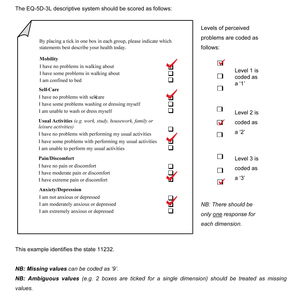
\includegraphics[width=.5\textwidth]{i/eq5d1.jpg}\hfill
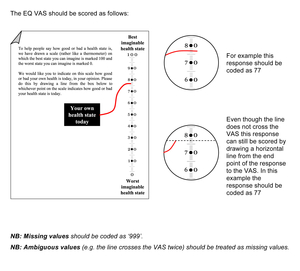
\includegraphics[width=.5\textwidth]{i/eq5d2.jpg}
\label{fig:eq5d}
\end{figure}

The EQ-5D has been shown to be useful for common mental health conditions such as mild to moderate depression \parencite{brazier2010eq}, which may well be appropriate for this system. However, it is possible that it suffers from an issue discussed in the section \ref{questionnairelength} above; it is too short. In fact, in the study by \citeauthor{crawford2011selecting}, it was this questionnaire that participants raised concerns about with regard to it being too short to properly assess complex outcomes \parencite{crawford2011selecting}.

\newpage
\subsection{Mental Health Recovery Star (MHRS)}
The \enquote{Mental Health Recovery Star} (MHRS) is part of a set of outcome measure tools called \enquote{Outcomes Stars} \parencite{outcomesstars}. It measures ten areas of a user's life, rating them on a scale of 1 to 10, where 1 is \enquote{stuck} and 10 is \enquote{self-reliance}. This then produces a graphic in the shape of a ten-pointed star, an example of which can be seen in Figure \ref{fig:mhrs} (image from \parencite{outcomesstars}):

\begin{figure}[ht]
\centering
\caption{The Mental Health Recovery Star}
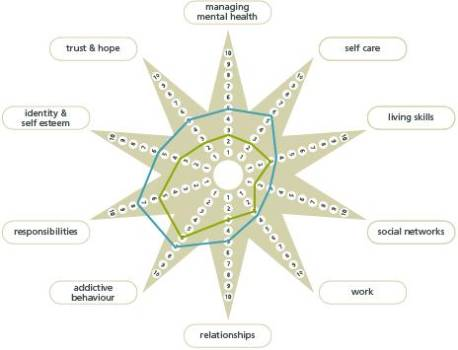
\includegraphics[width=\textwidth]{i/recoverystar.jpg}]
\label{fig:mhrs}
\end{figure}

This measure has been \enquote{received enthusiastically by both
mental health service providers and service users} \parencite{dickens2012recovery}. A study by \citeauthor{killaspy2012psychometric} (\citeyear{killaspy2012psychometric}) aimed to analyse the psychometric properties of the MHRS. This had some positive results, revealing that 85\% of participants found the MHRS useful in areas such as planning support and tracking their recovery. It also found that 70\% of participants said the MHRS was easy to use. However, this study only considered MHRS recorded either by staff or collaboratively with staff and user.

Staff or collaborative recording is common with the MHRS; many staff are given training in order to guide users in using the measure. In fact, training is now a requirement to gain a license to use the star \parencite{starlicense}. Clearly this poses an issue for this project. Assuming a license could be obtained without training (which may be unlikely), it is possible that this training issue could be overcome with computerised tutorials and careful user experience design. However, this would still require the user to learn how to use the MHRS, and would be more complicated than a more simple, intuitive outcome measure.

Another issue with MHRS is the time to complete. In the study by \citeauthor{killaspy2012psychometric} it was found that it, on average, took 30 to 60 minutes to complete \parencite{killaspy2012psychometric}. While this was posed as a positive in this study, it is likely a negative for the purposes of this project. Response burden needs to be considered with regard to the desired frequency of response. For this project, the aim is to have a high frequency of response, meaning users will be able to regularly record their wellbeing. This could be multiple times per week, once per day or even multiple times per day. 

When considering 30 to 60 minutes with regard to this high desired response frequency, this is quite a high response burden. As discussed in the questionnaire length and response burden section, this is a key problem for this project. Also, it is likely that this time will be even longer than 30 to 60 minutes, given that the user would be completing the MHRS on their own without the guidance of a trained member of staff.

\subsection{Warwick-Edinburgh Mental Wellbeing Scale (WEMWBS)}
The \enquote{Warwick-Edinburgh Mental Wellbeing Scale} (WEMWBS) is a scale designed to \enquote{enable the monitoring of mental wellbeing in the general population} \parencite{wemwbs}. It was developed by a panel of experts \parencite{wemwbsdevelopment} and has been tested fairly extensively, finding that it \enquote{showed good content validity} and is a \enquote{short and psychometrically robust scale} \parencite{tennant2007warwick}. It consists of 14 positively worded items with 5 possible responses to each, ranging from \enquote{none of the time} to \enquote{all of the time}.
\newpage
These questions and responses can be seen in Figure \ref{fig:wemwbs} (table from \parencite{wemwbsquestions}):
\begin{figure}[ht]
\centering
\caption{The Warwick-Edinburgh Mental Wellbeing Scale}
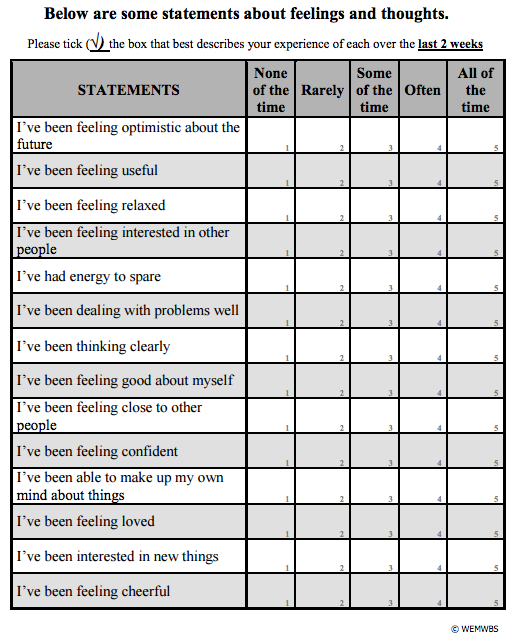
\includegraphics[width=.8\textwidth]{i/wemwbs.png}
\label{fig:wemwbs}
\end{figure}

The fact that WEMWBS was developed for the general population is particular useful to this project, as a general purpose, simple scale is exactly what this project requires. Another strength of this scale is that it produces a single score, which is simply a sum of the responses. Each response is scored 1-5, giving a score of 14-70 for the full questionnaire \parencite{wemwbsscoring}. This is beneficial to this project as a single score can be easily recorded and mapped against other data such as date/time, or user specific API data such as social media activity.

The study by \citeauthor{crawford2011selecting} (\citeyear{crawford2011selecting}) found the WEMWBS to be largely successful, in that it achieved one of the highest ratings among participants. This study identified another key problem with various outcome measures, which was the use of negatively phrased questions, as users said it can be \enquote{upsetting to be asked long lists of questions about difficulties associated with mental ill health}. The WEMWBS was commended by participants for phrasing items positively, where poor mental health would be recognised by a lack of these positive terms, rather than the presence of negative terms.

A problem with WEMWBS however is the length of the questionnaire, in that it consists of 14 items. This shouldn't be too time consuming for the user as the questions are not open ended, and are relatively simple. However, again regarding the aim of a high response frequency, a shorter questionnaire may be more effective for the purposes of this project. Thankfully, a shorter version of the WEMWBS exists; the \enquote{Short WEMWBS} (SWEMWBS).

\subsection{Short WEMWBS (SWEMWBS)} \label{swemwbssection}
The \enquote{Short WEMWBS} (SWEMWBS) is a shorter version of the WEMWBS, consisting of a 7 item scale rather than a 14 item scale \parencite{swemwbs}. The questions on the short version are a subset of those on the full version, so retain the advantages of being positively worded. In order to compare the two scales, the score obtained from the shorter version is mapped to a \enquote{metric} score via a conversion table. This conversion table can be seen in appendix \ref{swemwbsconversiontable}.
\newpage
The questions in the SWEMWBS can be seen in Figure \ref{fig:swemwbs} (table from \parencite{swemwbsquestions}):
\begin{figure}[ht]
\centering
\caption{The Short Warwick-Edinburgh Mental Wellbeing Scale}
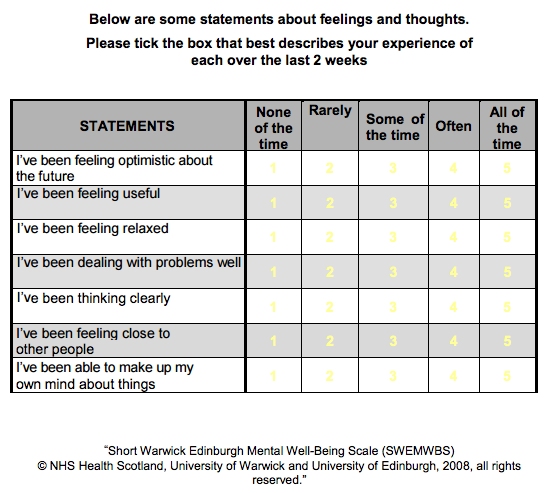
\includegraphics[width=.8\textwidth]{i/swemwbs.png}
\label{fig:swemwbs}
\end{figure}

The scale was developed in a research project by \citeauthor{stewart2009internal} (\citeyear{stewart2009internal}). This project tested the shorter scale and drew various conclusions on its validity and effectiveness. While the longer version of course provides more detail, the r-value was found to be 0.954 in the development and testing of the scale, meaning the scores produced are very similar. Given the high correlation of scores, the lower response burden and robust measurement properties of SWEMWBS, this testing found that this made \enquote{SWEMWBS preferable to WEMWBS at present for monitoring mental wellbeing in populations} \parencite{stewart2009internal}.

The disadvantages of this scale are that, as discussed, it does provide a more narrow view of a person's wellbeing. \citeauthor{stewart2009internal} (\citeyear{stewart2009internal}) found that where \enquote{face validity is an issue there remain arguments for continuing to collect data on the full 14 item WEMWBS}. However, for the purposes of this project a simpler scale with lower face validity is preferable.

The SWEMWBS (as well as the WEMWBS) is copyrighted by the University of Warwick and NHS Health Scotland. However, it is free to use as long as users register by completing a registration form \parencite{wemwbsreg}.

\subsection{This Project}
The SWEMWBS will be used for this project as it seems to provide a good trade off between response burden and obtaining meaningful measures of mental health and wellbeing. It is publicly available (after registration) and provides a single wellbeing score per response, which will aid massively when building visualisations. This will make mapping of wellbeing to other factors simple, which should result in simple, effective and easy to understand visualisations for the user.

\section{Personal Informatics} \label{personalinformatics}
\subsection{Introduction}
Personal informatics can be defined as software that is designed to \enquote{help individuals collect personal information to improve self-understanding}, allowing them to \enquote{promote positive behaviors} such as \enquote{healthy living, energy conservation, etc.} \parencite{li2012personal}.

\subsection{Stages of Personal Informatics}
A study by \citeauthor{li2010stage} (\citeyear{li2010stage}) developed a 5 stage model to represent personal informatics systems, consisting of \enquote{preparation, collection, integration, reflection, and action}.
\newpage

This study produced a diagrammatic representation of these stages, which is shown in Figure \ref{fig:5stagespi}.
\begin{figure}[ht]
\centering
\caption{Five Stage Model of Personal Informatics}
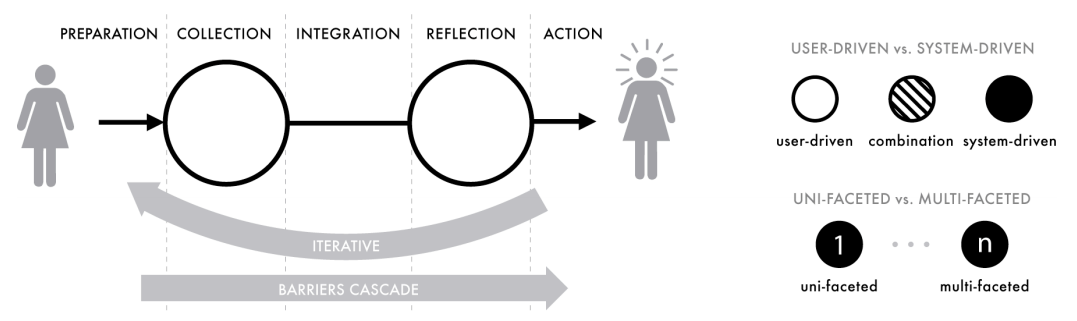
\includegraphics[width=\textwidth]{i/5stagespi.png}
\label{fig:5stagespi}
\end{figure}

\subsubsection{Preparation}
This section refers to the user's decision to start using a personal informatics tool, and their decision of which tool to use. This can cause issues when users do not prepare sufficiently. It can result in users switching between applications, which can cause issues where \enquote{they abandon their previous data
because most systems do not support data exporting}, or \enquote{if they can export data, the formats between the applications
may not be the same} \parencite{li2010stage}.

This project hopes to minimise the risk of this, in that most of the data used will not be entered by the user, but rather pulled from existing applications such as Twitter and Strava. It also hopes to reduce this by recording wellbeing in a way that is already developed and in circulation; the SWEMWBS scale \parencite{swemwbs}. However, this stage is not the main focus of this project.

\subsubsection{Collection}
This stage is, as expected, the stage where people collect information about themselves. There are two key methods of collection: active and passive. That is, either the user has to enter information themselves, or it is recorded automatically.

Active collection can result in problems where users \enquote{lacked time, lacked motivation, or did not remember to collect information} \parencite{li2010stage}. In the case of US health apps, \citeauthor{krebs2015health} (\citeyear{krebs2015health}) found that \enquote{about half of the respondents (427/934, 45.7\%) had stopped using some health apps, primarily due to high data entry burden, loss of interest, and hidden costs}. It is for this reason that some applications \enquote{are beginning to shift from requiring active tracking to
support for passive tracking} \parencite{rooksby2014personal}.

An aim of this project is to implement a solution that combines these two types of collection, and results in a form of compromise. If most data is collected from applications the user already uses, this can be viewed as passive collection in the context of this system (even if the user actively recorded this data on another system). This means that the active collection within this system can be kept as small as possible (just the SWEMWBS questionnaire).

It is possible that in the future wearable technologies will be able to track wellbeing, which could make collection entirely passive. Research is ongoing in this area, for example a project by \citeauthor{valenza2014wearable} (\citeyear{valenza2014wearable}) developed a system to \enquote{recognize four possible clinical mood states in bipolar patients ... using heart rate variability information exclusively}. Interesting as this is, it is outside of the scope of this project. It may however be identified as an area for future work.

\subsubsection{Integration}
This stage combines and transforms data for the user. The amount of user input that is required varies, but in the case of this project this should require no user involvement. The system should already have wellbeing data, and user credentials for external applications, so should be able to integrate the data automatically.

\subsubsection{Reflection}
This stage involves the user interrogating their data, and being presented with visualisations in order to reflect on the data. Building these visualisations in an effective way is not easy. \citeauthor{keim2008visual} (\citeyear{keim2008visual}) stated that while \enquote{the capacity to collect and store new data rapidly grows, the ability to analyze these data volumes increases at much lower rates}.

Presentation and visualisations are large challenges for this project, and will be discussed further in section \ref{visualisations}.

\subsubsection{Action}
This stage relates to how users respond to the reflection stage. \enquote{Some systems alert the user to take
actions} based on some arbitrary criteria \parencite{li2010stage}. However, this project will leave this section entirely user driven, in order to limit the scope of the project, and to avoid giving any sort of clinical advice.

\subsection{Types of Data Tracked}
A huge number of people are collecting and recording data about themselves, whether this is by choice or is automatic. For example, it is reported that there are approximately 15 million Twitter users in the UK, and around 60\% of the UK population has a Facebook account \parencite{smdemographics}. These applications record lots of data about users, but this is usually not the primary reason people use social media. In fact, a study by \citeauthor{whiting2013people} (\citeyear{whiting2013people}) found that there are ten key reasons people use social media: \enquote{social interaction, information seeking, pass time, entertainment, relaxation,
communicatory utility, convenience utility, expression of opinion, information sharing, and
surveillance/knowledge about others}. Information storage is clearly a requirement and side product of many of these, but is not the primary motivation.

In terms of self-tracking by choice, a study by \citeauthor{krebs2015health} (\citeyear{krebs2015health}) reported that, in the US, 58.23\% of smartphone users \enquote{had downloaded a health related mobile app}. It also found that most participants used these apps \enquote{at least daily}.

There are many examples of applications that collect data, falling into various categories. Two examples of these categories are: exercise data on apps like Strava \parencite{strava} and social media activity data on apps like Facebook \parencite{facebook} or Twitter \parencite{twitter}. These forms of personal informatics applications will be discussed later, with regard to their relevance to mental health and wellbeing.

This data is collected for a number of reasons, such as:
\begin{itemize}
\item To tailor content to the user, whether that content be trends, adverts, suggested \enquote{accounts} or suggested \enquote{friends}.
\item To report statistics such as how much the user has exercised, and whether they have hit certain targets. Note that this encompasses more areas of personal informatics than the above reason. It allows the user to not only collect data about themselves, but to carry out some analysis on the data.
\end{itemize}

It is important to recognise all of this results is a huge amount of data being collected, which is available for analysis. A paper by \citeauthor{swan2013quantified} (\citeyear{swan2013quantified}) defined the \enquote{quantified self}, or QS, as \enquote{the selftracking of any kind of biological, physical, behavioral, or environmental information}. This paper stated that future \enquote{QS applications could include tools for rendering QS data meaningful in behavior change}. Clearly there is desire to make use of all of this data, and to allow users to interpret and make behavioural changes based on the quantified self.

\section{Personal Informatics in the Context of Mental Health and Wellbeing} \label{personalinformaticsmentalhealth}
Lots of personal informatics data relates to mental health and wellbeing, and personal informatics is said to offer \enquote{great potential to more effective management of clinical
mental health problems} \parencite{pimentalhealth}. This project will consider two types of data, and two applications that collect these types of data about users. Both of the applications considered have open Application Programming Interfaces (APIs) for accessing a user's data, given the user's credentials.

\subsection{Physical Exercise}
\subsubsection{Link to Mental Health}
Physical exercise has long been linked with mental health; a study in 1990 stated that in \enquote{general, findings from research indicate that exercise is associated with improvements in mental health including mood state and self-esteem} \parencite{raglin1990exercise}. More recently, another study found that \enquote{exercise is beneficial for mental health; it reduces anxiety, depression, and negative mood, and improves self-esteem and cognitive functioning} \parencite{callaghan2004exercise}.

\citeauthor{canzian2015trajectories} (\citeyear{canzian2015trajectories}) investigated this relationship by monitoring users' locations at various points, calculating values such as distance travelled, and comparing this data to the results of daily mood questionnaires. This study found \enquote{that there exists a significant correlation between mobility trace characteristics and the depressive moods}, and managed to produce \enquote{models that are able to successfully predict changes in the depressive mood of individuals by analyzing their movements}.

\subsubsection{Strava}
Strava is a mobile app that \enquote{lets you track your running and riding with GPS, join Challenges, share photos from your activities, and follow friends} \parencite{stravamobile}. It was reported in March 2015 to have had about 8.2 million users, 1.2 million of which can be classed as active \parencite{stravausers}, so is clearly a very popular and active app.

Strava also has an API \parencite{stravaapi}, that allows retrieval of a users activities, which is perfect for the needs of this system.

\subsection{Social media}
\subsubsection{Link to Mental Health}
A project by \citeauthor{de2013predicting} (\citeyear{de2013predicting}) stated that \enquote{social media contains useful signals for characterizing the onset of depression in individuals}. This same project managed to build a classifier using Twitter data, to predict onset depressive episodes in patients with major depression, with an impressive accuracy of around 70\%.

On the other hand, a study by \citeauthor{hawn2009take} (\citeyear{hawn2009take}) stated that incorporating social media in healthcare is \enquote{one route to greater patient happiness - and to a more patient-centered health care system}. Another article stated that Facebook usage \enquote{may contribute to an overall sense of connection and wellbeing. However, given the research on social media, it is evident that certain ways of using and experiencing Facebook are complex and potentially harmful} \parencite{smhurtorhelp}.

While most research seems to express concerns about negative affects of social media usage on mental health, other studies talk of positive impacts. Either way it is clear that social media activity has some affect on mental health and wellbeing, so is an interesting and important type of data to be included in this system.

\subsubsection{Twitter}
This project will incorporate Twitter data. According to Twitter, the platform has 313 million active users \parencite{twitterabout}. Facebook is a larger social media platform, with around 1.79 billion active users \parencite{facebookusers}, but Twitter provides a more simple, restricted dataset.

Simply mapping number of tweets to wellbeing may be more effective than trying to map friends, statuses, activity, events and other data to wellbeing. The latter option could lead to the \enquote{sheer volume of analysis overwhelming the sense-making process itself}, an issue that was found in a paper by \citeauthor{jones2016sensemaking} (\citeyear{jones2016sensemaking}). Also, the success of the project by \citeauthor{de2013predicting} (\citeyear{de2013predicting}), in building a classifier with Twitter data, provides proof that Twitter data will be useful in this context.

Again, Twitter provides a simple API for retrieving user data such as user timelines, allowing for retrieval of tweets \parencite{twitterrestapi}. It also provides a search API for more complex searches \parencite{twittersearchapi}.

\section{Visualisations} \label{visualisations}
Deciding how to present the user with visualisations is a huge challenge for this project, and is a key area of the field of personal informatics in which this project hopes to contribute. \citeauthor{jones2016sensemaking} (\citeyear{jones2016sensemaking}) investigated the challenges of sensemaking for personal informatics in a health context.

This study identified various challenges:
\begin{enumerate}
\item Overwhelming of users with too much data.
\item Poor presentation of information leading to misinterpretation.
\item Lack of transparency in outputs.
\item Difficulty of obtaining holistic insights from disjointed outputs.
\end{enumerate}

Challenge 3 is more related to how the data is collected, and should hopefully be overcome by the collection method (SWEMWBS) as discussed earlier in this literature survey.

It seems that challenge 2 and 4 are caused primarily by the system trying to predict which visualisations the user will find useful. In terms of challenge 2, it was found that, for the system tested, \enquote{numerous examples of the phraseology ... [lead] to misinterpretation}. For challenge 4, one participant tried \enquote{to understand the associations between the quality of her sleep, the temperature at night, and her mood}. It was found that the system tested \enquote{provided few explicit mechanisms to support this linking activity}.

Predicting what the user will find useful is clearly difficult, which may be solved by providing lots of visualisations. However, this method can lead to challenge 1: overloading of information. This is the case with Exist, as will be discussed in section \ref{exist}.

The solution that this project will trial to overcome these three challenges (1, 2 and 4) is: do not try to predict the visualisations the user wants, but rather implement a tool allow the user to build custom visualisations themselves. That is, allow the user to select which data sources they want to be included in the displayed visualisation.

\section{Existing Systems} \label{existingsystems}
This section will focus on systems that interpret and produce visualisations. While there are similar systems from the context of data collection, the collection system for the proposed project is a very small, simple part of the overall system. Also, the justification of collection method has been discussed already in section \ref{whichoutcomemeasures} above.

This section will consider four similar systems, and discuss the similarities and differences between each system and the system proposed in this project.

\subsection{Optimism}
Optimism \parencite{optimism} is similar to the proposed system from a mental health context. It allows users to self track their mood, wellbeing and many other things, in order to self-manage their mental health this way. Optimism apps are designed for users with Depression, Bipolar, Anxiety or PTSD.

\newpage
Some images of the optimism system can be seen in Figure \ref{fig:optimism} (images from \parencite{optimism}):
\begin{figure}[ht]
\centering
\caption{Optimism Web App}
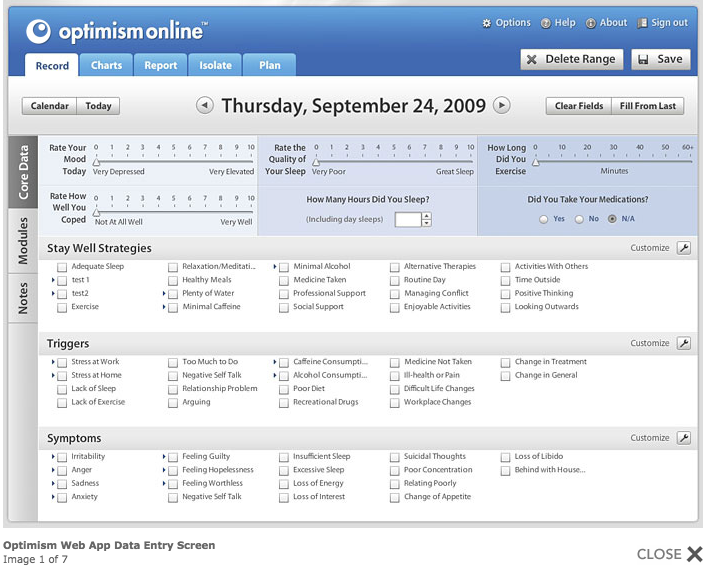
\includegraphics[width=.5\textwidth]{i/optimism1.png}\hfill
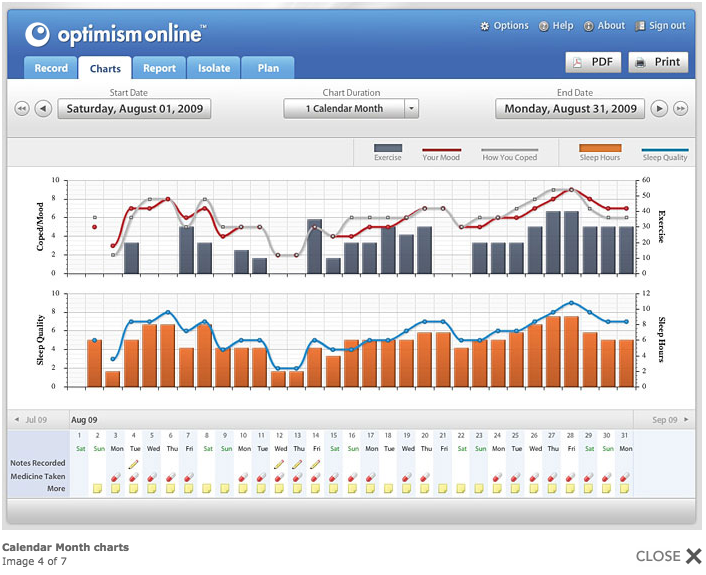
\includegraphics[width=.5\textwidth]{i/optimism2.png}
\label{fig:optimism}
\end{figure}

While Optimism is similar in it's aims to this project, it is a more \enquote{heavy duty} mental health management app, whereas the proposed system in this project is a more lightweight, general purpose self-management app. Optimism clearly has a significantly higher response burden than the proposed system in this project. It does have a wider array of features, but while this can be a positive in terms of aiding users, it means that users will need to spend time learning how to use and interpret the system.

Also, a key part of the proposed system is making use of data that already exists about a user (via existing application APIs), which is a feature not included in Optimism.

\subsection{Exist} \label{exist}
Exist \parencite{exist} is similar to the proposed application from an API data import context. It also produces visualisations of this data, but with some key differences. It imports API data, then produces a dashboard of correlations rather than allowing the user to build visualisations themselves. While Exist is not designed for health or mental health tracking, it has the potential to be used for this, and is actually very impressive in terms of analysing the correlations in data.

There are various issues with Exist however. The study by \citeauthor{jones2016sensemaking} (\citeyear{jones2016sensemaking}) that investigated challenges in sensemaking, was in fact carried out using Exist. The various pre-built visualisations, as well as lack of customisation, can result in users not being able to interpret their data effectively.

\subsection{Zenobase}
Zenobase \parencite{zenobase} is similar to the proposed system from both an API data import and visualisation building context. Zenobase allows users to \enquote{store, aggregate and visualize your data}. It again imports API data, but unlike Exist allows users to build custom visualisations from this data.

This is similar to the functionality of the proposed system. A feature of note that Zenobase has, that is not yet planned for the proposed system, is the ability to manually import data. This means that Zenobase could, while significantly more difficult and time consuming, be used in the exact same way as the proposed system for self-management of mental health and wellbeing.

The system proposed in this project instead has the ability to record a very restricted amount of user data through the SWEMWBS questionnaire. While this simplicity is an advantage of the proposed system, allowing users to also manually import of data would be a nice addition. This may have to be identified as future work.

Zenobase seems to be extremely flexible, and allows the user to interrogate their data in a large number of ways. As a side effect of this, it is quite complex to use and understand. Having tested the system, this does not seem to be due to the design, but due to the flexibility and large number of ways that Zenobase allows users to visualise their data.

This flexibility is clearly an advantage for those users that want it, and the proposed project would not hope to compete with Zenobase in this respect. However, the higher difficulty and complexity may not be accepted by all users, especially those that are not willing to spend the time learning to use a fairly complex system to be able to interrogate their data.

\subsection{Fluxstream}
Like Zenobase, Fluxstream \parencite{fluxstream} also allows users to provide API credentials (via \enquote{connectors}), import their data, and build visualisations from this imported data.

Fluxstream consists of two core applications: a Calendar app and a BodyTrack app. The first of these divides visualisations into various \enquote{tabs}, such as a clock, dashboards, a map and a timeline. This seems to encounter the same challenge as exist: too many options of data interpretation are being provided simultaneously.

It does seem to be very powerful in collating data. The timeline feature for example can be used to map the data from lots of \enquote{connectors}, allowing the user to view all of their activity in one \enquote{feed}. However, the complexity of comprehending the data may deter some users.

The BodyTrack app includes a \enquote{grapher}, allowing the user to build custom visualisations.

An image of this can be seen in Figure \ref{fig:fluxstream} (image taken from video on \parencite{fluxstream}):
\begin{figure}[ht]
\centering
\caption{Fluxstream BodyTrack Grapher}
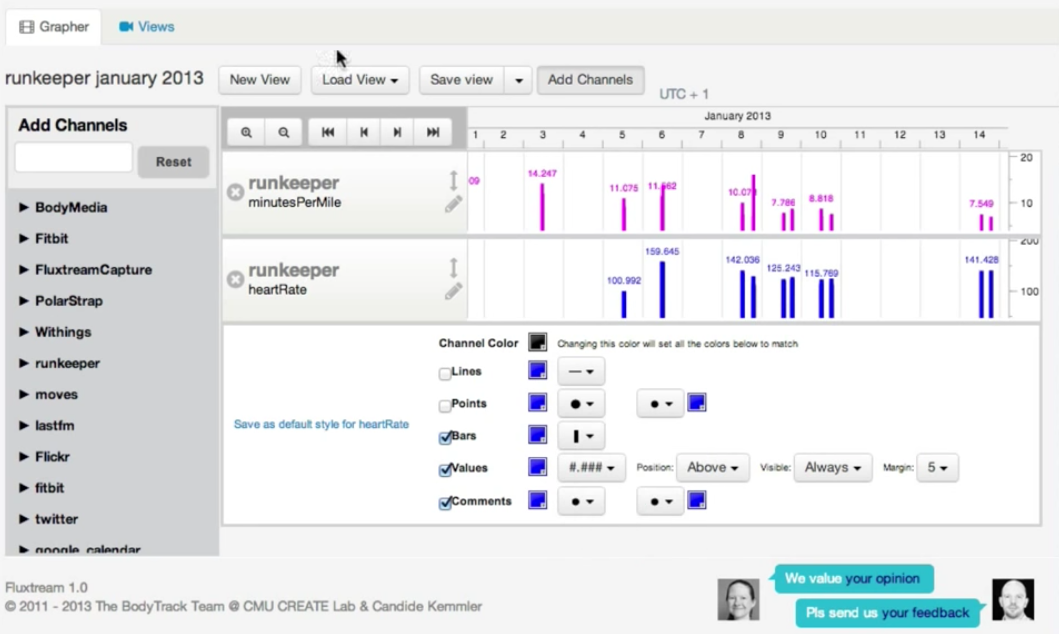
\includegraphics[width=\textwidth]{i/fluxstream.png}
\label{fig:fluxstream}
\end{figure}

This again seems very flexible, but also complicated and very difficult to use, which could again turn users away from the system.

Another issue is that there doesn't seem to be a way to record or import data manually into Fluxstream. Also, Fluxstream does not currently support any mental health and wellbeing tracking apps. This means that it may be impossible, or at least very difficult, for users to use Fluxstream as a mental health tracking/self management tool.

\newpage
\subsection{Summary}
The four systems reviewed in this section were similar to the proposed system in varying ways. Reviewing these existing systems provided some extremely useful insights as to how the proposed system can differentiate itself from similar systems. A summary of these insights is provided below:
\begin{itemize}
\item The system will combine user submitted mental health and wellbeing data with API data.
  \begin{itemize}
  \item None of the systems reviewed do this explicitly.
  \item Optimism allows user submitted mental health data, but no API data.
  \item The other three apps allow importing of API data, but no mental health data.
  \item The closest to allowing this is Zenobase, which allows manual data importing. This however would be harder and more time consuming for the user, and would require them to develop their own way of measuring their wellbeing.
  \end{itemize}
\item The system will include a \emph{simple} visualisation building tool.
  \begin{itemize}
  \item Exist and Optimism generated (fairly) fixed visualisations.
  \item Zenobase and Fluxstream included very flexible, complex and difficult to use visualisation building and customisation tools.
  \item The proposed system could, when compared to Zenobase and Fluxstream, sacrifice flexibility to make the system easier to use and understand.
  \end{itemize}
\end{itemize}

\chapter{Requirements Specification}
\section{Introduction}
This chapter will detail the functional and non functional requirements for the various areas of the system. These requirements were obtained and developed primarily from existing research in the area, as discussed in detail in chapter \ref{litsurvey}, as well as from personal experience and desires for the project. They will encompass the results of the literature survey, and the aims and objectives discussed in sections \ref{aims} and \ref{objectives} respectively. Most of the requirements are unambiguous and intuitive, based on the sources just discussed. However, where a requirement seemed vague and/or its origins seemed to be unclear, an additional sentence or two has been included to justify the requirement, and explain both where it came from and why it is necessary.

Many projects develop requirements from user interviews and surveys, but this wasn't done for this project for various reasons. Firstly, this is an academic project, so is better suited to requirements based on existing literature. Secondly, a goal of this system was to provide a proof of concept that can be built on in the future, rather than a full working system. It may be  advantageous in the development of requirements for future work to consult potential users from the various user groups. There are many possible users, such as those who do not suffer from a diagnosed mental health condition, those that are not in treatment, those that are in treatment and those that are post-treatment. The opinions of all of these may be useful for future work and improvements to the system, but for this project only academic research, personal experience and desires for the project were considered, in order to limit the scope of the project and produce an extensible system for future research and development.

\section{Requirements Structure and Terminology}
\subsection{Structure}
This project will consist of the development of three separate software systems: a mobile app, a web app and an \enquote{application programming interface} (API). These systems are intentionally designed to be entirely separate from one another, as will be discussed further in chapter \ref{chap:design}. This is important to mention here because, as a result of this, the requirements are divided into three separate sections; one for each of the separate software systems. Each of these sections is then divided into functional and non-functional requirements, where functional requirements describe \enquote{what the system does}, and non-functional requirements describe \enquote{how the system works}.

\subsection{Prioritisation Terminology}
These requirements use the \enquote{MoSCoW} method for prioritisation \parencite{moscowmethod}. This is a technique that consists of the terminology seen in Table \ref{table:moscow} (term descriptions derived from \parencite{moscowmethod}).

\begin{table}[ht]
\centering
\caption{MoSCoW Method for Requirements Prioritisation Terminology}
\label{table:moscow}
\begin{tabular}{|p{4cm}|p{10cm}|}
\hline
\textbf{Term} & \textbf{Description} \\ \hline
Must have & These are needed for the \textbf{M}inimum \textbf{U}sable \textbf{S}ubse\textbf{t} (\textbf{MUST}) of requirements. That is, they are absolutely required for the system to be viable. Without them, the system does not fulfil a primary goal, provides no value, or is unsafe in some way. \\  \hline
Should have & These are important but not absolutely vital. If they are not completed, some workaround may be possible. The system will still be viable and usable, but may be inefficient or awkward to use. \\ \hline
Could have & These are desirable but not as important as \enquote{should have} requirements. They very much depend on time constraints, and can often be dropped if deadlines are approaching. Although they improve the system, they are not really necessary for the system to be viable. \\ \hline
Won't have this time & These are explicitly defined as requirements that will not be met by the system in this release. Explicitly defining these is useful for limiting the scope of a project/release, as it prevents ambiguity and prevents these requirements from being introduced as extra work at a later date. \\ \hline
\end{tabular}
\end{table}

\newpage
This project is of course, like many projects, time limited. This method of prioritisation was extremely useful in defining and limiting scope, deciding which functionality should be implemented first, and deciding what could be dropped should problems occur and/or time constraints apply.

\subsection{Further Terminology}
The requirements also refer to \enquote{major} and \enquote{minor} bugs. These are defined in Table \ref{table:bugsterminology}.
\begin{table}[ht]
\centering
\caption{Major and Minor Bugs Terminology}
\label{table:bugsterminology}
\begin{tabular}{|p{4cm}|p{10cm}|}
\hline
\textbf{Bug} & \textbf{Description} \\ \hline
Major & These cause the system to not meet the requirement in question, or meet the requirement but significantly impact the system in some other way, such as security issues, or major user experience issues. For example, if information shifts \enquote{off-screen}, and so is invisible to the user, this is a fairly major user experience issue. \\  \hline
Minor & These are unintended, but the system still meets the requirement in question, and the consequences are not particularly severe. For example, if content shifts and makes information difficult to read, or simply makes the software look unprofessional. This is undesirable, but still a fairly minor issue, so would be classed as a minor bug.\\ \hline
\end{tabular}
\end{table}

\section{Requirements} \label{reqs}
\subsection{Mobile App}
The mobile app is intended to be very small and simple. It is not a mobile version of the web app, but is instead a simple piece of software to allow users to record their wellbeing quickly using their phone (and hence carry out ecological momentary assessment, as discussed in section \ref{sec:ema}). For this reason, there are a fair amount of \enquote{won't} requirements, in order to keep the software simple and limit the scope. That being said, the requirements for the mobile app are as follows:

\subsubsection{Functional}
\begin{enumerate}
\item Must allow the user to log in.
\item Must allow the user to log out.
\item Should allow the user to create an account.
\item Must allow the user to record their wellbeing.
  \begin{enumerate}
  \item Must have a SWEMWBS questionnaire (see section \ref{swemwbssection}).
  \item Must submit total score of SWEMWBS questionnaire.
  \end{enumerate}
  \item Must submit date and time with wellbeing score.
\item Could have a recent wellbeings table, displaying user's recent wellbeing recordings.
\item Should encourage user to visit the web app to connect existing apps and analyse their wellbeing data.
\item Won't have ability to manage user account.
  \begin{enumerate}
  \item Won't have ability to change user email.
  \item Won't have ability to change user password.
  \item Won't have ability to recover password.
  \end{enumerate}
\item Won't have ability to connect existing apps.
\item Won't have ability to produce and view visualisations.
\end{enumerate}

\subsubsection{Non-functional}
\begin{enumerate}
\item Should allow users to access the SWEMWBS questionnaire within 4 'taps' (email, password, log in, record). Note this of course does not include typing of email and password.
\item Must be built using \enquote{React Native} \parencite{reactnative} \parencite{reactnativegit} to maximise cross-platform code reuse between iPhone and Android.
\item Should include documentation for developers on how to set up the project and get it running.
\item Must be tested manually on iOS (iPhone), including testing by volunteer testers.
  \begin{enumerate}
  \item Must reveal no major bugs when testing all \enquote{must} requirements.
  \item Should reveal no minor bugs when testing all \enquote{must} requirements.
  \item Should reveal no major bugs when testing all \enquote{should} requirements.
  \item Could reveal no minor bugs when testing all \enquote{should} requirements.
  \item Should reveal no major bugs when testing all \enquote{could} requirements, if these features are implemented.
  \item Could reveal no minor bugs when testing all \enquote{could} requirements, if these features are implemented.
  \item Should also be tested (by volunteer testers) with the goal of identifying missing features, bugs not relating to defined requirements, and usability issues.
  \end{enumerate}
\item Could be effective on Android due to the software being built using React Native.
  \begin{enumerate}
  \item Won't be tested manually on Android.
  \end{enumerate}
\end{enumerate}

\subsection{Web App}
The web app is significantly larger, and incorporates most of the major contributing features of this project, including connecting existing apps and building and viewing visualisations. The web app does almost everything, if not everything,% the mobile app does, and more. Also note that security is not discussed here, as all data is accessed via the API, so security is a requirement of the API, not the web app.

\subsubsection{Functional}
\begin{enumerate}
\item Must allow the user to log in.
\item Must allow the user to log out.
\item Must allow the user to create an account.
\item Must allow the user to record their wellbeing.
  \begin{enumerate}
  \item Must have a SWEMWBS questionnaire (see section \ref{swemwbssection}).
  \item Must submit total score of SWEMWBS questionnaire.
  \end{enumerate}
\item Must submit date and time with wellbeing score.
\item Should encourage user to download the mobile app to record their wellbeing from their phone.
\item Should allow user to manage user account.
  \begin{enumerate}
  \item Should allow user to change user email.
  \item Should allow user to change user password.
  \item Could allow user to recover password.
  \item Could allow user to verify their email.
  \end{enumerate}
\item Must keep user logged in throughout navigation of application.
\item Should keep user logged in after full page refreshes.
\item Must allow user to connect their Twitter account.
  \begin{enumerate}
  \item Must store this information for use in subsequent requests to Twitter's API, to fetch user's data.
  \item Must be able to fetch user's tweets.
  \end{enumerate}
\item Must allow user to connect their Strava account.
  \begin{enumerate}
  \item Must store this information for use in subsequent requests to Strava's API, to fetch user's data.
  \item Must be able to fetch user's Strava data.
  \end{enumerate}
\item Won't include connection of any applications other than Twitter and Strava, as these are the only sources being included as proofs of concept.
\item Must be able to fetch user's SelfReflect wellbeing data.
\item Must allow user to build visualisations combining any of these three sources of data (SelfReflect wellbeing data, Twitter data and Strava data).
  \begin{enumerate}
  \item Must provide one visualisation built from SelfReflect wellbeing data.
  \item Must provide one visualisation built from Twitter data.
  \item Must provide one visualisation built from Strava data.
  \item Should allow Twitter and Strava data to be directly compared to SelfReflect wellbeing data in some way, via these visualisations.
  \item Could also allow all three data sources to be directly compared with one another in some way, via these visualisations.
  \item Won't include interactive visualisations (such as \enquote{zoom}, \enquote{click and drag} etc.).
  \end{enumerate}
\item Should provide a guide/help page for the user, with a \enquote{step-by-step} guide on how to use the system.
\end{enumerate}

\subsubsection{Non-functional}
\begin{enumerate}
\item Must be built using React \parencite{react} and Redux \parencite{redux}, meaning it is built almost entirely in JavaScript.
\item Should be a \enquote{one page} application. That is, built using AJAX (asynchronous JavaScript and XML) requests only. This means there will be no full page requests after the initial request. This is what allows separation of functional requirements 8 and 9.
\item Should use ReactD3 to build visualisations, which is an open source library for building charts using React \parencite{reactd3}.
\item Should incorporate and be styled using Skeleton CSS, which is a \enquote{dead simple, responsive boilerplate} \parencite{skeletoncss}.
\item Could be responsive due to the use of Skeleton CSS. That is, the application will adjust styling and work on various screen sizes. Note this is easily tested by simply resizing browser windows. Hence:
  \begin{enumerate}
  \item Could work on mobile phones.
  \item Could work on tablets.
  \item Should be tested on various browser window sizes to test responsiveness.
  \end{enumerate}
\item Should include documentation for developers on how to set up the project and get it running.
\item Must be tested manually, including testing by volunteer testers.
  \begin{enumerate}
  \item Must reveal no major bugs when testing all \enquote{must} requirements.
  \item Should reveal no minor bugs when testing all \enquote{must} requirements.
  \item Should reveal no major bugs when testing all \enquote{should} requirements.
  \item Could reveal no minor bugs when testing all \enquote{should} requirements.
  \item Should reveal no major bugs when testing all \enquote{could} requirements, if these features are implemented.
  \item Could reveal no minor bugs when testing all \enquote{could} requirements, if these features are implemented.
  \item Should also be tested (by volunteer testers) with the goal of identifying missing features, bugs not relating to defined requirements, and usability issues.
  \end{enumerate}
\end{enumerate}

\subsection{API} \label{subsec:apireqs}
The API is the server; it is where storage and retrieval of all user data happens. It is a huge part of the system and is the source of many important features such as user management, wellbeing data storage and retrieval, connection of existing applications, fetching of data from existing applications and security/authentication.

\subsubsection{Functional}
\begin{enumerate}
\item Must allow creation of users.
\item Should allow fetching of users.
\item Should allow update of users.
  \begin{enumerate}
  \item Should allow update of email.
  \item Should allow update of password.
  \item Could allow deletion of users.
  \item Could allow password recovery.
  \item Could allow verification of user email.
  \end{enumerate}
\item Must allow storage of SWEMWBS wellbeing score.
  \begin{enumerate}
  \item Must allow storage of data and time of submission with wellbeing score.
  \item Must include a copy of the SWEMWBS conversion table, as seen in appendix \ref{swemwbsconversiontable}
  \item Must be able to convert raw to metric SWEMWBS score, using this table.
  \end{enumerate}
\item Must allow retrieval of recent SWEMWBS metric wellbeing scores, with date and time.
  \begin{enumerate}
  \item Could allow specification of how many score entries to return.
  \end{enumerate}
\item Must allow connection and storage of Twitter credentials
\item Must allow retrieval of user's recent tweets, if they have connected Twitter. This should be exactly as defined by Twitter's API, and not modified in any way.
\item Must allow connection and storage of Strava credentials.
\item Must allow retrieval of user's recent Strava data, if they have connected Strava. This should be exactly as defined by Strava's API, and not modified in any way.
\item Won't include connection of any applications other than Twitter and Strava, as these are the only sources being included as proofs of concept.
\item Must accept and return data as JSON (JavaScript Object Notation).
\item Must require authentication for any request that returns a user's data.
  \begin{enumerate}
  \item Must allow user to provide a valid email and password in exchange for an authentication access token.
  \item Must require a valid token to access user's data (i.e. all requests other than requests to create a user, or requests for a token).
  \item Could allow refreshing of tokens before they expire, by allowing user to provide a valid token in exchange for a fresh one.
  \item Must prevent users from accessing other user's data, or any other restricted data, regardless of access token.
  \end{enumerate}
\end{enumerate}

\subsubsection{Non-functional}
\begin{enumerate}
\item Must be built using Node.js (a JavaScript runtime for writing server side JavaScript code) \parencite{nodejs} and Express (a \enquote{fast, unopinionated, minimalist web framework for Node.js}) \parencite{expressjs}. These are modern tools that will both speed up development and likely produce faster, more reliable, higher quality code. Node.js is very popular and, as a result, there exists lots of compatible open source software compatible that this project can take advantage of.
\item Must use MySQL for database access (the \enquote{world's most popular open source database}) \parencite{mysql}. There is little reason to use anything else for database access for this project, as MySQL is suited for all the project's needs. There are alternatives, but for the purposes of this project, these would not provide any significant benefits over MySQL.
\item Must store passwords in a secure, hashed format. This is so that, even if this database is somehow accessed, user's passwords will not be lost.
\item Should be a RESTful API. REST is Representational State Transfer and employs a stateless architecture where each request is independent. This is a modern standard and best practise for building APIs. This stateless architecture means each request must be authenticated individually. Endpoints are implemented as resources such as \emph{/users/} and are accessed using http \enquote{verbs} (GET, POST, PUT, PATCH, DELETE) \parencite{httpmethods}.
\item Must include extensive documentation that satisfies the following requirements:
  \begin{enumerate}
  \item Must include documentation for developers on how to set up the project and get it running.
  \item Must have documentation for all endpoints. This is absolutely essential to make the API professional and, more importantly, to make the entire SelfReflect system extensible. Developers must understand the API, be able to use the API, and be able to extend the API if this project is to be built upon in the future.
  \end{enumerate}
\item Should have automated tests. This section of the project deals with user data and security, so correct and reliable behaviour is essential. Also, while the API can be manually tested indirectly via the web and mobile apps, it cannot be manually tested directly, so automated tests are important.
  \begin{enumerate}
  \item Should have automated tests covering at least 70\% of lines of testable code.
  \item Could have automated tests covering at least 95\% of lines of testable code.
  \end{enumerate}
\end{enumerate}

\chapter{Design} \label{chap:design}
This chapter will detail the design of both the system as a whole, and the three separate parts of the system (mobile app, web app and API), with regard to the requirements specified in section \ref{reqs}. Functional and non-functional requirements from this point onwards will be referred to as \enquote{F} and \enquote{NF} requirements respectively. Requirements referenced in each section will always refer to the corresponding section in section \ref{reqs}, unless explicitly stated. This chapter should cover all of the requirements in section \ref{reqs}, except for those that relate to testing and documentation, as they will be covered in the testing and implementation chapters respectively.

\section{Overall System}
Many modern software systems are designed using a client-server architecture. That is, one server and many clients, such as for web pages. Additionally, many successful applications have external APIs, which allow developers of external applications to build their own interfaces to the data, accessed via the corresponding API. These are the same APIs this project will take advantage of in order to fetch user data from existing applications, such as Twitter and Strava.

The system developed in this project will take a similar approach to this client-server, API based design. Most systems developed using these methods include internally developed client applications, that access the data differently from externally developed applications. The system in this project however will not do this. The mobile and web apps will access the data entirely via the API, and as such will essentially be no different to applications developed externally by other developers, as shown in Figure \ref{fig:OverallSystem}. This encourages, and to an extent guarantees, maximum extensibility for the project. The internally developed client applications will have the same access to the data as externally developed applications, meaning there is no disparity between the abilities of internally and externally developed client applications.

\begin{figure}[ht]
\centering
\caption{Overall System Architecture}
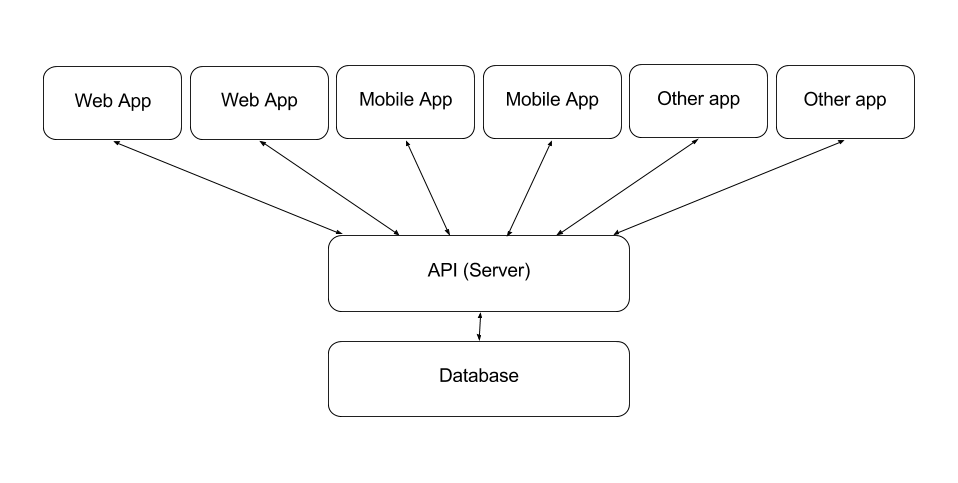
\includegraphics[width=\textwidth]{i/OverallSystem.png}
\label{fig:OverallSystem}
\end{figure}

\newpage
\section{Mobile App}
One internal client application that will communicate via the API is the SelfReflect mobile app. This is a fairly simple application, with the primary goal of allowing the user to record their mental health and wellbeing easily via a mobile app, in order to facilitate ecological momentary assessment.

This application will be built using \enquote{React Native} \parencite{reactnative}. React Native is a framework for building native mobile apps using JavaScript. It uses the same native components that are used when developing in Objective-C or Java (for iOS and Android respectively), but uses JavaScript to assemble them. A huge advantage of this is that almost all code, if not all code, is cross-platform. This is the reason for NF2, NF4 and NF5. Although the mobile app will only be tested on iOS, it may well be as (or almost as) effective on Android, purely by virtue of the technologies used to build it.

To facilitate the design of the mobile app, various \enquote{wireframes} were created to provide some plan as to how the application should look. These are low fidelity prototypes, and images of each will be included and referenced throughout this section.

\subsection{Login and Register}
The first page the user sees after opening the mobile app will be a simple login screen, with email and password fields, and two buttons: one to login, and one to navigate to a register screen. The wireframe for this screen can be seen in Figure \ref{fig:mobilelogin}.

\begin{figure}[ht]
\centering
\caption{Mobile App Login Screen Wireframe}
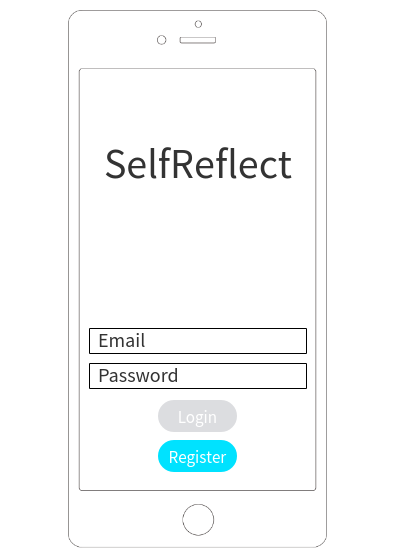
\includegraphics[width=0.3\textwidth]{i/mobilelogin.png}
\label{fig:mobilelogin}
\end{figure}

The user can then either log in, satisfying F1, or navigate to the register screen, satisfying F3. The wireframe for the register screen can be seen in Figure \ref{fig:mobileregister}.

\begin{figure}[ht]
\centering
\caption{Mobile App Register Screen Wireframe}
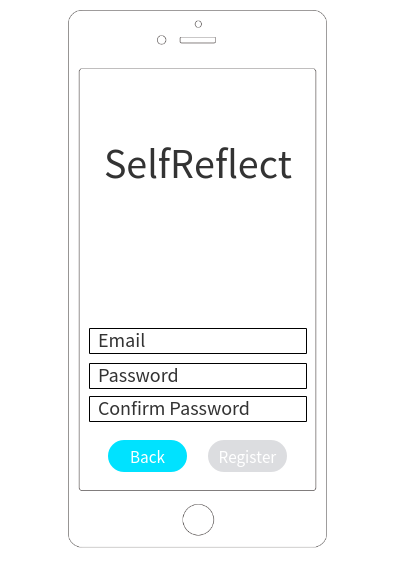
\includegraphics[width=0.3\textwidth]{i/mobileregister.png}
\label{fig:mobileregister}
\end{figure}

Both logging in and registering will then need to communicate with the SelfReflect API, in order to either create the user in the SelfReflect database, or to validate login credentials before allowing the user to log in. The mobile app must therefore be able to handle both successful and erroneous responses from the API (such as invalid password, email already exists, server error etc.), and give the user some feedback on these.

A successful login will result in the API responding with an access token (see section \ref{sec:apisecurity}). This will then have to be stored locally in the mobile app's state, so that it can be sent with subsequent requests, as discussed in the following sections.

\subsection{Home Page}
After logging in successfully, the user will be taken to the home page. This page will include:
\begin{enumerate}
\item A table of recent recordings, satisfying F6. Note this is a \enquote{could} requirement, so may be dropped if time constraints apply.
\item A message to encourage the user to visit the SelfReflect web app, satisfying F7.
\item A button to navigate to a SWEMWBS questionnaire, to record wellbeing.
\end{enumerate}

Also note that all pages (once logged in), will contain a button at the top of the page to log out of the app, satisfying F2. The wireframe for this home page can be seen in Figure \ref{fig:mobilehome}.

\begin{figure}[ht]
\centering
\caption{Mobile App Home Screen Wireframe}
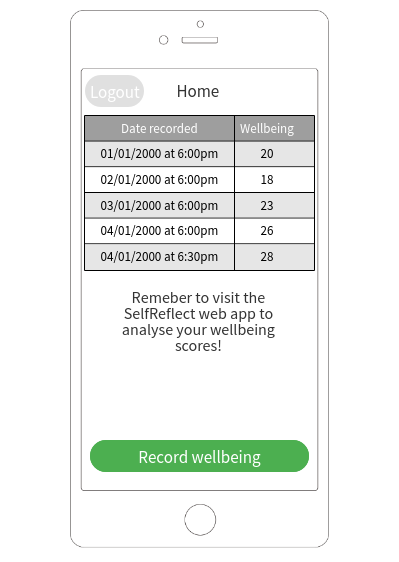
\includegraphics[width=0.3\textwidth]{i/mobilehome.png}
\label{fig:mobilehome}
\end{figure}

The table of recent recordings on this screen is, of course, dynamically generated as it is fetched from the API. As discussed earlier, this will require the mobile app to make a request to the API, using the access token obtained from the user logging in. The API will then respond with the user's recent recordings, and the table can be generated.

Also, the button to record wellbeing satisfies NF1, as it allows users to get to the SWEMWBS questionnaire in 4 taps. These are: tap email (then input), tap password (then input), tap login, tap record button.

\subsection{SWEMWBS Questions}
If the user taps the \enquote{record wellbeing} button, they will navigate to the SWEMWBS questions, satisfying F4.1. As mobile screens are small, the questions will be presented to the user one at a time. All of these question screens will be similar, so only one wireframe was created, as can be seen in Figure \ref{fig:mobilequestion}. In this wireframe, \enquote{often} has been selected as an answer, hence the green background.

\begin{figure}[ht]
\centering
\caption{Mobile App SWEMWBS Question Screen Wireframe}
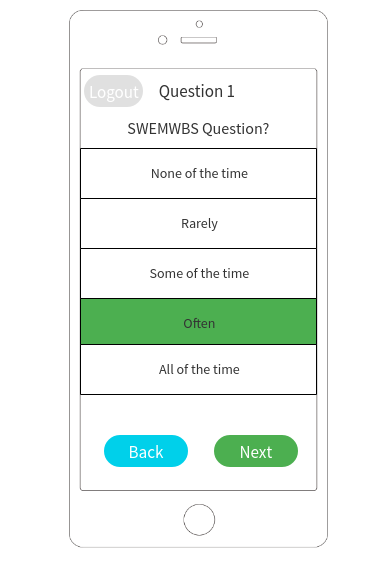
\includegraphics[width=0.3\textwidth]{i/mobilequestion.png}
\label{fig:mobilequestion}
\end{figure}

The only small difference between different question screens is that the last question screen will contain a \enquote{submit} button, rather than a \enquote{next} button. Note that all questions are mandatory; the next buttons (and the submit button) will be disabled until the question on that page has been answered.

The submit button will sum the answers to all the questions and submit these via the SelfReflect API, satisfying F4.2. It will also compute the date and time of submission, and submit this alongside the computed wellbeing score, satisfying F5. It is important to compute this \enquote{client-side} rather than \enquote{server-side}, as this is (to the user) when the wellbeing was recorded. If this was computed server-side and some delay happened, the user could end up with a wellbeing recorded at a time significantly different from when they actually tapped submit. Computing this client-side makes this almost impossible, as long as date and time are computed and communicated correctly.

\section{Web App} \label{sec:webappdesign}
The second, larger internal client application that will communicate via the API is the SelfReflect web app. This is much more complex and has many more features than the mobile app. It allows everything the mobile app allows, but also enables the user to connect existing apps and produce visualisations from their data, fetched from both the SelfReflect API and other connected existing apps (Twitter and Strava). Again, wireframes were created to facilitate the design of the web app, and will be included and referenced throughout this section.

\subsection{Choice of Technologies}
This application will be built in \enquote{React} \parencite{react} and \enquote{Redux} \parencite{redux}, satisfying NF1. React is a JavaScript framework/library, and Redux is a tool and development methodology for handling state in JavaScript applications. There are a huge number of potential advantages to incorporating both of these: faster software, more modular/functional code, shorter development time, better extensibility and various others. This is true for various frameworks however, not just React. 

React was chosen over other frameworks for various reasons, such as personal experience and preference, React's popularity, and various other advantages it provides over other frameworks. However, this project is not about with the benefits of React, or the comparison of JavaScript frameworks, so will not discuss these reasons in too much detail. For the purposes of this project, selecting some JavaScript framework was the important, and React and Redux were chosen due to personal experience, preference and knowledge of the current state of the field of JavaScript web development.

Building the entire application in React means that all navigation will happen via updates to application state, rather than full page requests. This means the web app will be \enquote{one page}. That is, the original request will fetch the entire application, then the displayed page will simply depend on the state, which is updated via user actions. Server requests therefore will be made asynchronously, via \enquote{AJAX} requests. This satisfies NF2, and can create an interesting and smooth user experience compared to traditional web pages, as users never have to wait for full page refreshes.

\subsection{Styling and Responsiveness}
As with almost all web pages, CSS (Cascading Style Sheets) will be used to style the content of the web application. It is possible to write all CSS from scratch. However, there are a huge number of libraries to aid with styling, so as to reduce development time, and to make certain problems easier, such as producing responsive websites. The most popular of these is likely Bootstrap, developed at Twitter \parencite{bootstrapcss}. Bootstrap is a huge library that provides a great number of features: a \enquote{grid system}, styling for many base components, custom components, and jQuery plugins. However, this project will use Skeleton CSS instead \parencite{skeletoncss}. Skeleton also provides a simple grid system, and styling for some base and custom components. It is massively more lightweight than Bootstrap, while still providing everything this project requires.

The grid system in these libraries is the feature that supports responsiveness of websites, allowing them to work on different sized screens. All elements are placed within the grid, which is twelve \enquote{columns} wide. The grid resizes as the screen size changes, so if there are not enough \enquote{free} columns for an element, it is placed on the next \enquote{row}. This should mean that using Skeleton CSS will satisfy NF4, NF5.1 and NF5.2, as long as the grid system is used correctly.

\subsection{Home}
The first page the user sees when loading the web app is the home page, which contains some information about the project as a whole, and buttons to navigate to log in and register. The wireframe for this is seen in Figure \ref{fig:webhome}.

\begin{figure}[ht]
\centering
\caption{Web App Home Screen Wireframe}
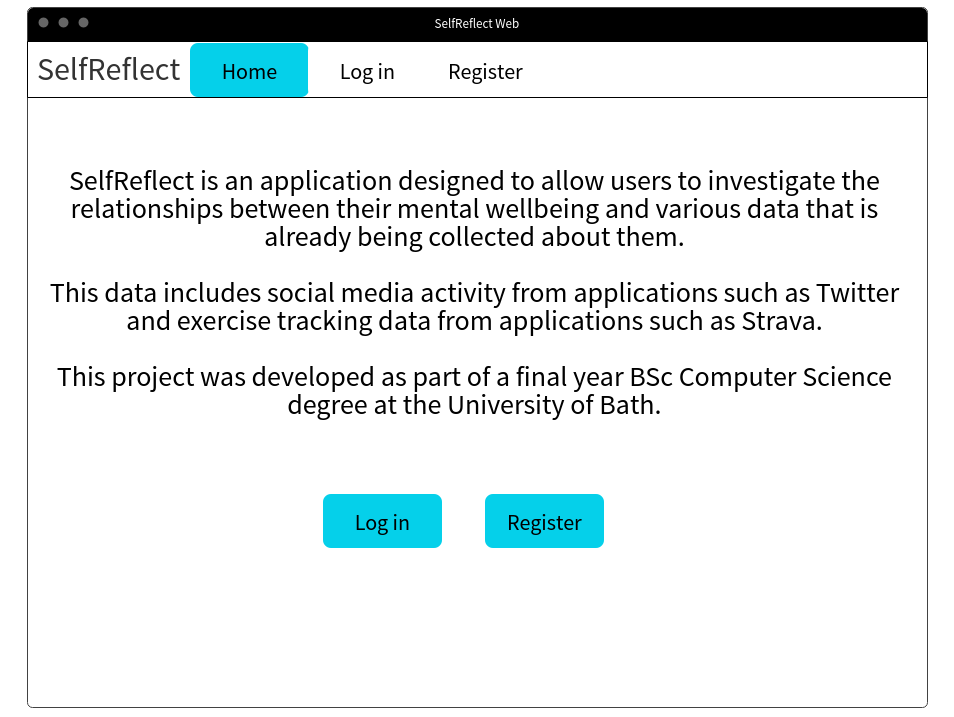
\includegraphics[width=0.8\textwidth]{i/webhome.png}
\label{fig:webhome}
\end{figure}

\newpage
\subsection{Login and Register}
If the user clicks log in (either the button on the home page, or on the navigation bar), they will be directed to the login page, satisfying F1. The wireframe for this can be seen in Figure \ref{fig:weblogin}.

\begin{figure}[ht]
\centering
\caption{Web App Login Screen Wireframe}
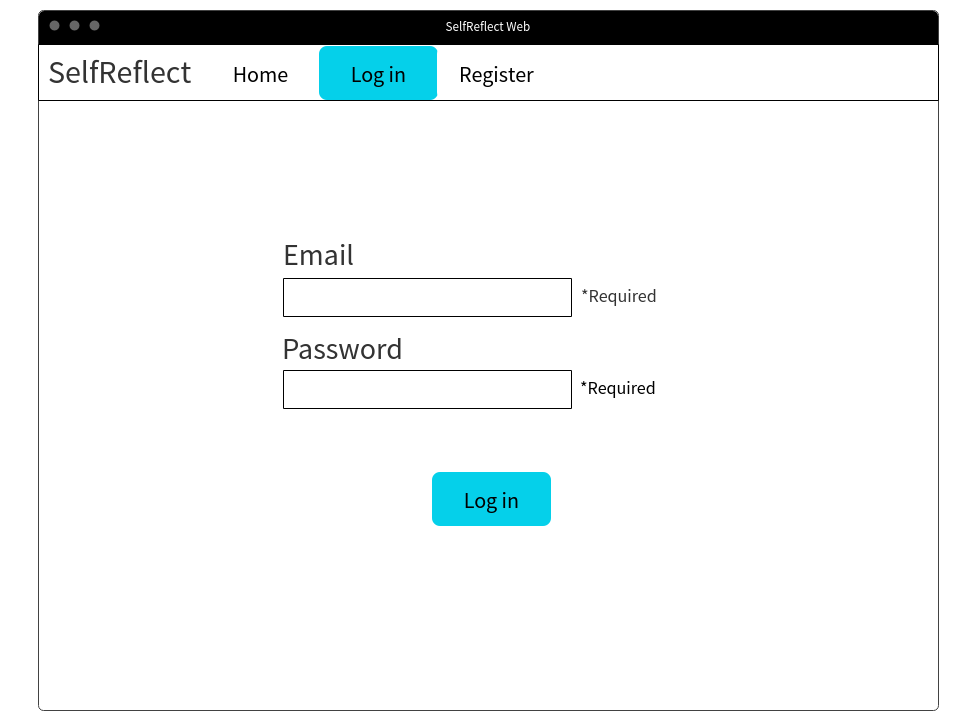
\includegraphics[width=0.8\textwidth]{i/weblogin.png}
\label{fig:weblogin}
\end{figure}

\newpage

If the user clicks register (again either the button on the home page, or on the navigation bar), they will be directed to the register page, satisfying F3. The wireframe for this can be seen in Figure \ref{fig:webregister}.

\begin{figure}[ht]
\centering
\caption{Web App Register Screen Wireframe}
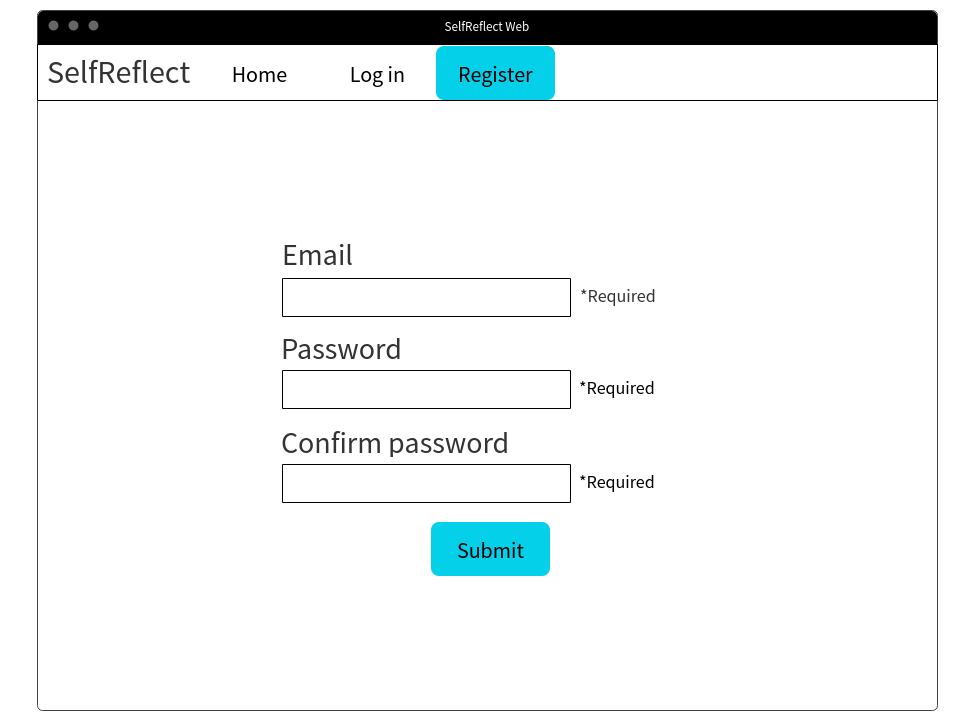
\includegraphics[width=0.8\textwidth]{i/webregister.png}
\label{fig:webregister}
\end{figure}

Exactly as with the mobile app, both logging in and registering involve requests to the SelfReflect API. Again, this means the web app must be able to handle and give feedback on both successful and erroneous responses from the API. Also, again like the mobile app, the web app must store the access token it obtains somewhere, for use in subsequent requests.

Token storage is a little more complicated for the web app however. Simply storing the token in the state of the web application satisfies F8, as the user can be logged in as long as the token exists and is valid. However, if the token is only stored in state, as soon as the user refreshes the page the token will be lost, which fails F9. This kind of persisted login behaviour is usually achieved through the use of \enquote{HTTP cookies} in web applications. However, cookies are sent in the header of every request automatically, which is not intended for this application. Thankfully, modern browsers provide \enquote{HTML Local Storage} \parencite{htmllocalstorage}, which allows applications to store data in the browser, and retrieve this data whenever they desire. This will be used in this project to satisfy F9. The web app will store the access token in local storage, retrieve it on page load, and hence allow persisted login for users in much the same way as using cookies.

\subsection{Guide}
After a valid login, the navigation bar changes and the user is automatically directed to the guide page, satisfying F15. The wireframe for this is shown in Figure \ref{fig:webguide}.

\begin{figure}[ht]
\centering
\caption{Web App Guide Screen Wireframe}
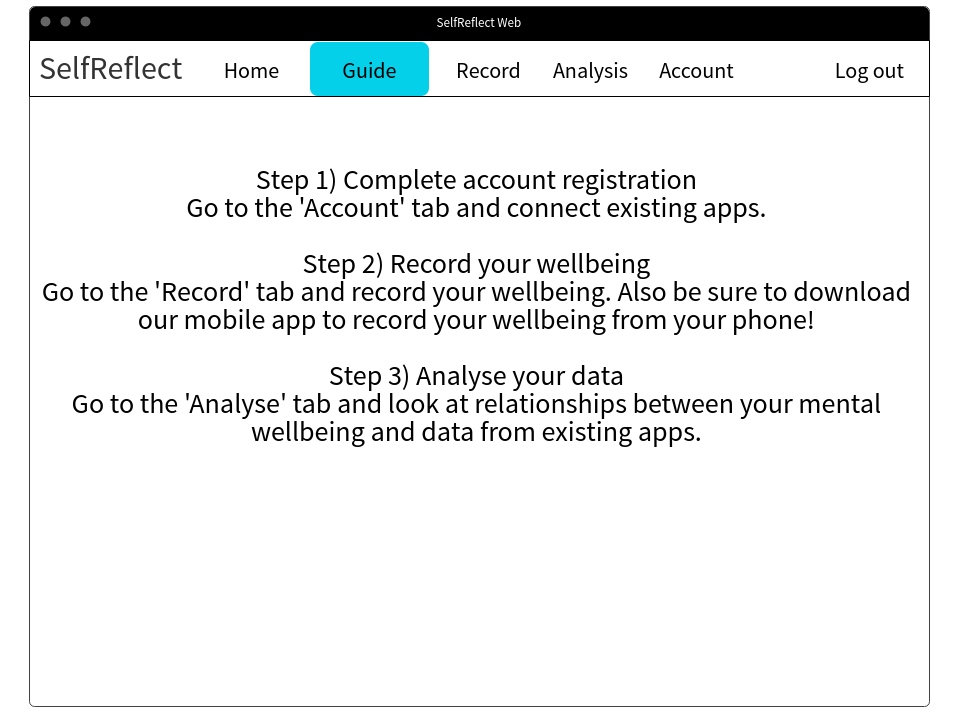
\includegraphics[width=0.8\textwidth]{i/webguide.png}
\label{fig:webguide}
\end{figure}

Similar to the mobile app, all subsequent screens have a log out button in the top right corner, satisfying F2. Note this guide page also includes a prompt to download and use the SelfReflect mobile app, satisfying F6.

\subsection{SWEMWBS Questionnaire}
Clicking the record button will navigate the user to the SWEMWBS questionnaire, satisfying F4.1. This is on one page, and allows the user to scroll up/down as they select answers to each of the seven questions. At the bottom of the page there is a submit button which computes and submits total score, satisfying F4.2. Exactly like the mobile app (and for the same reasons), this also computes date and time of submission, satisfying F5. The wireframe for this page can be seen in Figure \ref{fig:webrecord}. This image only shows the bottom of the screen. The first 4 questions are \enquote{off-screen} to the top.

\begin{figure}[ht]
\centering
\caption{Web App SWEMWBS Questionnaire Screen Wireframe}
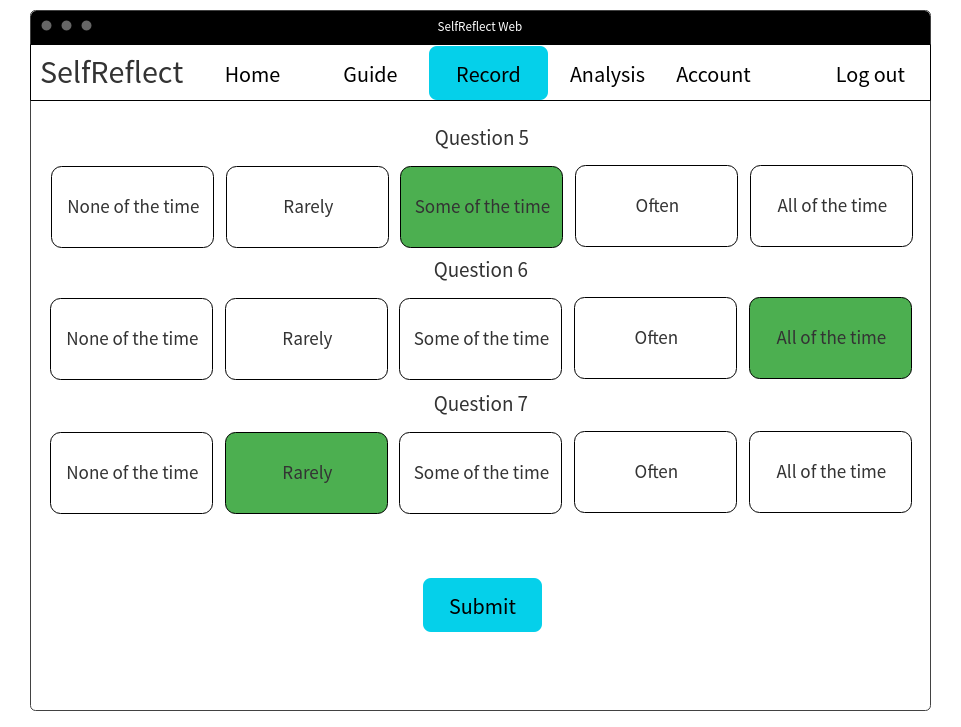
\includegraphics[width=0.8\textwidth]{i/webrecord.png}
\label{fig:webrecord}
\end{figure}

\subsection{Account Management} \label{sec:webaccman}
The account screen will allow the user to edit their account details and connect existing apps. The wireframe for this page can be seen in Figure \ref{fig:webaccount}.

\begin{figure}[ht]
\centering
\caption{Web App Account Screen Wireframe}
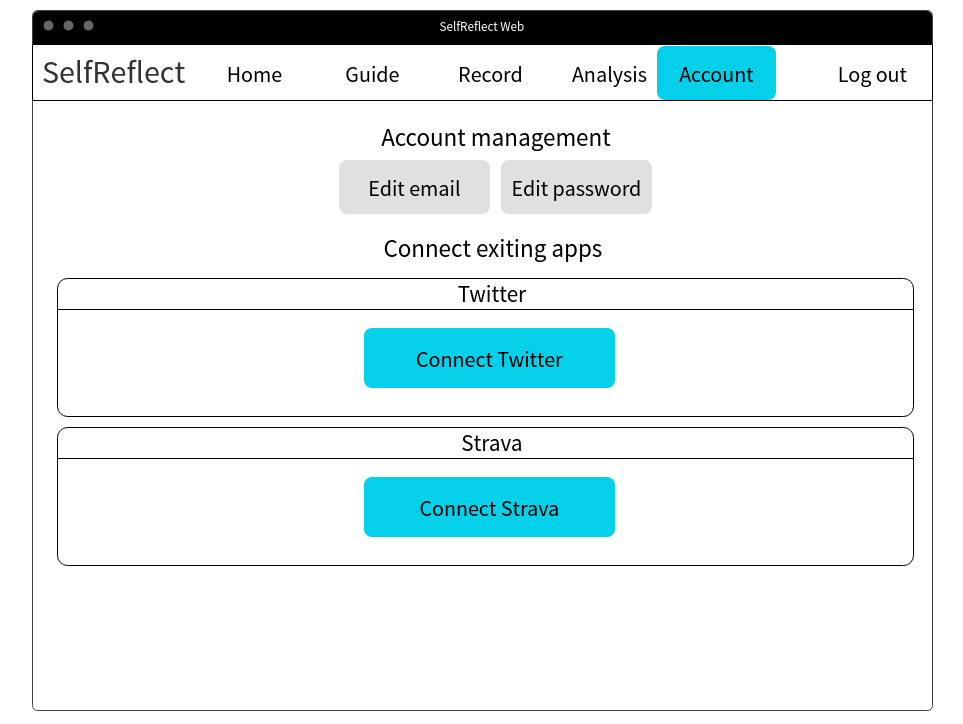
\includegraphics[width=0.8\textwidth]{i/webaccount.png}
\label{fig:webaccount}
\end{figure}

The edit email and edit password buttons will reveal simple forms that allow the user to update their email and password respectively. This satisfies F7.1 and F7.2. The connect Twitter and connect Strava buttons will direct the user to the required pages (from Twitter and Strava) to provide their credentials and connect the corresponding app. When the apps are connected, the access credentials returned from these apps will be sent to the SelfReflect API for storage, so that user data can be fetched from these apps later. This satisfies F10.1 and F11.1.

\newpage
\subsubsection{A Note on Unmentioned Requirements}
Password recovery (F7.3) and email verification (F7.4) are not planned in the account management section, or any section, of the web app design. In carrying out the design and planning phase of this project, time constraints seemed to be fairly tight given the scale of the software development being undertaken. As these requirements were both \enquote{could} requirements, and neither would contribute academically to the research or findings of this project, both were considered not worth the time taken for development, and so were dropped at the design phase.

\subsection{Analysis and Visualisations}
The analysis page allows the user to select which sources they wish to include in their visualisation, then press generate to build and display the visualisations. The wireframe for this page can be seen in Figure \ref{fig:webanalysis}

\begin{figure}[ht]
\centering
\caption{Web App Analysis Screen Wireframe}
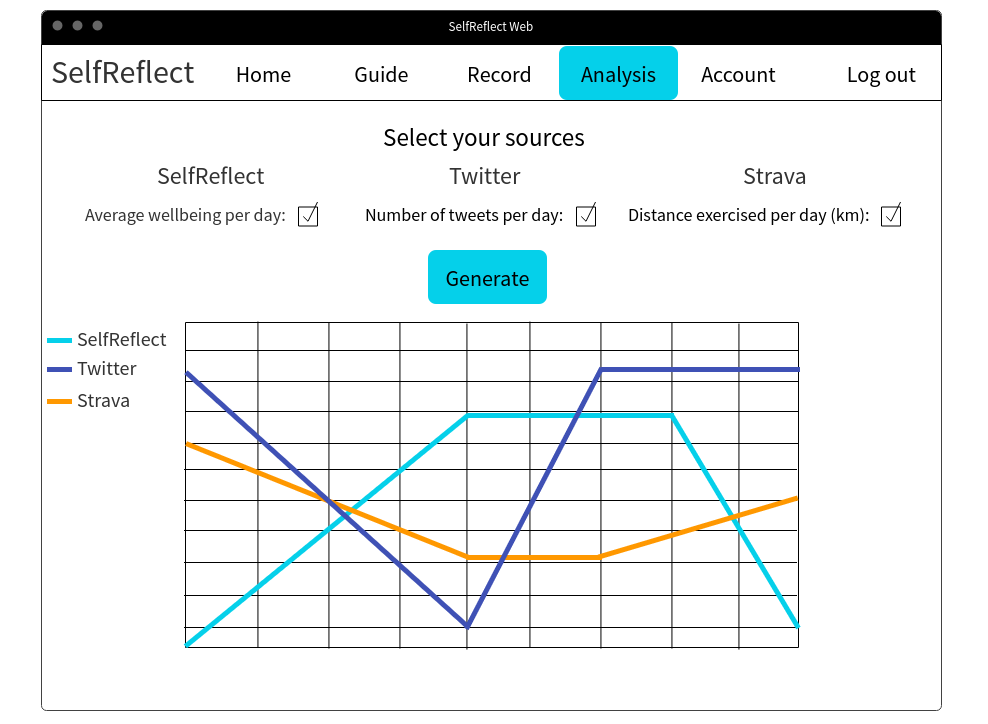
\includegraphics[width=0.8\textwidth]{i/webanalysis.png}
\label{fig:webanalysis}
\end{figure}

\newpage
This will fetch data from SelfReflect, Twitter and Strava via the SelfReflect API, satisfying F13, F10.2 and F11.2. It will then process this data and build a graph with the selected visualisations included. The three chosen visualisations will be:
\begin{enumerate}
\item Average wellbeing per day from SelfReflect data.
\item Number of tweets per day from Twitter data.
\item Distance exercised per day (km) from Strava data.
\end{enumerate}

This satisfies the requirements to have one visualisation per source (F14.1, F14.2 and F14.3). Also, as all of these visualisations consist of integer numbers that are likely to be somewhat compatible, they can all be plotted on one graph, as shown in the wireframe. This therefore allows external sources to be compared with both SelfReflect, and with one another, hence satisfying F14.4 and F14.5.

These visualisations will be built using an open source project called \enquote{ReactD3} \parencite{reactd3}, satisfying NF3. This allows charts to be built fairly easily within the React framework, as long as data is provided in a compatible format. Making use of this library will significantly reduce development time, and will take advantage of the developmental effort, experience and testing that has already been carried out for this open source project.

\section{API} \label{sec:apidesign}
The API is the server of SelfReflect's client-server type model. It handles all data storage, user management, connecting of existing apps, fetching of existing apps data and security/authentication.

\subsection{Choice of Technologies}
\subsubsection{JavaScript Object Notation (JSON)}
JSON will be both the accepted and returned format of data for the API, satisfying F11. This is a simple \enquote{key-value} format that is lightweight, popular and is of course very easy to process in JavaScript. This is a clear advantage to this project as all three software systems will be written in JavaScript. An example JSON object can be seen below:
\begin{lstlisting}
{
  "id": 1,
  "email": "email@example.com"
}
\end{lstlisting}

\subsubsection{Node.js}
The API will be developed using \enquote{Node.js} \parencite{nodejs}. Node.js is a JavaScript runtime that allows server side code to be written using JavaScript. As \enquote{an asynchronous event driven JavaScript runtime, Node is designed to build scalable network applications} \parencite{nodejsabout}. It is massively successful and popular, and as such there exists lots of compatible open source software for Node.js.

\subsubsection{Express}
Much like the mobile and web apps, and for many of the same reasons (development time, extensibility, faster, more modular code etc.), a framework will be used for the API. This is a framework specifically for Node.js called \enquote{Express} \parencite{expressjs}. This will significantly reduce development time, and Express claim that \enquote{creating a robust API is quick and easy} \parencite{expressjs}. Using these technologies therefore satisfies NF1.

The justification for the choice of these technologies, and particularly of Express as a framework, is much the same as the justification for choosing React and Redux for the web app. This project is not researching the advantages and disadvantages of the various technologies, so while lots of research could be carried out and discussed, it would not be academically relevant to this project. These technologies were therefore chosen based on personal experience, preference and knowledge of the current state of the field of server side JavaScript and API development.

\subsubsection{MySQL}
MySQL will be used for database access, satisfying NF2. As discussed in NF2, there are many options for database access that satisfy this project's needs, so for the purposes of this project it was simply important to select one. MySQL was chosen purely due to personal experience, as this will likely reduce development time at no additional cost.

\subsection{RESTful API}
The API will be \enquote{RESTful}, satisfying NF4. \enquote{REST} is an architectural development methodology for APIs, and is said to \enquote{induce desirable properties, such as performance, scalability, and modifiability, that enable services to work best on the Web} \parencite{oraclerest}. For these and other reasons, REST is a popular, common best practise standard for building APIs.

REST is a stateless architecture, meaning all requests are independent from one another. This does pose a particular issue with regard to persisted login; most web applications handle persisted login via the use of sessions. These store some state on the server against some session identifier, then send cookies containing these session identifiers to clients. Clients then send these with every request and hence can remain logged in. However, this violates the stateless principle of REST. Storing access tokens on the server after a user has \enquote{logged in} would also violate this principle. This is a problem that requires a fairly subtle solution, and will be discussed in more detail in the Security and Authentication section (section \ref{sec:apisecurity}) later.

Probably the most important aspect of REST is the methodology used to design how a client accesses the API. REST uses http \enquote{verbs} (GET, POST, PUT, PATCH, DELETE) \parencite{httpmethods} to access \enquote{resources} via \enquote{Uniform Resource Identifiers} (URIs), producing an interface that is usually very intuitive. Any resource that accesses data should map almost identically to the database table it accesses. For example, SelfReflect has users, so will likely have a users table in the database and a resource at \emph{/users}. Creation of a users would then consist of a POST request to this resource, whereas simply fetching user details would consist of a GET request to something like \emph{/users/1}, where 1 is the requested user's unique identifier in the database. Each of the http \enquote{verbs} can be seen in Table \ref{table:httpverbs}, with a description of what they are typically used for in RESTful APIs.

\begin{table}[ht]
\centering
\caption{HTTP Verbs Usage in RESTful APIs}
\label{table:httpverbs}
\begin{tabular}{|p{2cm}|p{12cm}|}
\hline
\textbf{Verb} & \textbf{Usage} \\ \hline
GET &  To read a resource. Should not make any changes to data.  \\  \hline
POST & To create a new resource. Data of resource to be created is sent in body of the request.\\  \hline
PUT &  To update an existing resource. Usually the entire resource at this URI is replaced with the data sent in the body of the request, so the entire resource needs to be sent. If no resource exists at this URI, often one will be created, which is equivalent to a POST request to this URI.\\  \hline
PATCH & To modify an existing resource. This allows only a subset of the data in a resource to be sent in the body of the request, so that only the specified fields will be updated.\\  \hline
DELETE & Deletes a resource. \\  \hline
\end{tabular}
\end{table}

\newpage
\subsection{Endpoints} \label{sec:apiendpoints}
This section will define the endpoints that will be implemented for the API,  how to access each of them, and which requirements each of the endpoints satisfies. These can be seen in Table \ref{tab:designendpoints}. Security and restriction of endpoints will not be discussed in this section (F12.2 and F12.4); see section \ref{sec:apisecurity} for how this will be handled.

\begin{longtable}{| p{6cm} | p{6cm} | p{2cm} |}
\caption{API Planned Endpoints}
\label{tab:designendpoints} \\
\hline
\textbf{Endpoint} & \textbf{Description} & \textbf{Req(s) satisfied} \\ \hline
POST /users & Creates a new user. & F1 \\ \hline
GET /users/:id & Gets information about a user with the given id. & F2 \\ \hline
PUT /users/:id & Updates a user with the given id. & F3.1, F3.2 \\ \hline
DELETE /users/:id & Deletes the user with the given id. & F3.3 \\ \hline
POST /users/:id/wellbeings & Stores (creates) a new recorded wellbeing, including data and time of recording. This will accept the raw score and store it against metric score, based on a static conversion table stored in the database. See section \ref{sec:databasedesign} for details. & F4, F4.1, F4.3. \\ \hline
GET /users/:id/wellbeings?count=X & Gets a users recorded wellbeings, including data and time of recording. This will return \enquote{X} number of recordings, or fewer if less than X exist. There will need to be some sensible limit on X, such as 100. & F5, F5.1\\ \hline
PUT /users/:id/twitter-credentials & Stores (creates) a user's Twitter access credentials. Note this will be an access token of some sort, not the user's username and password. & F6 \\ \hline
GET /users/:id/tweets & Get a user's recent tweets. & F7 \\ \hline
PUT /users/:id/strava-credentials  & Stores (creates) a user's Strava access credentials. Note this will be an access token of some sort, not the user's username and password.& F8 \\ \hline
GET /users/:id/strava-data  & Get a user's recent Strava exercise data. & F9 \\ \hline
POST /tokens & Get an access token. Must provide a valid username and login for SelfReflect. This will be discussed further in the section \ref{sec:apisecurity}. & F12.1 \\ \hline
PUT /tokens & Refresh an access token. Must provide a valid access token. This will be discussed further in the section \ref{sec:apisecurity}. & F12.3 \\ \hline
\end{longtable}

\subsubsection{A Note on Unmentioned Requirements}
As discussed in the web app design section, password recovery (F4.5) and email verification were dropped (F3.5). See section \ref{sec:webaccman} for justification of this.

\subsection{Security and Authentication} \label{sec:apisecurity}
Data protection is incredibly important for any application that stores data about users. It is even more important for data that is sensitive, such as healthcare data, or in this case mental health and wellbeing data. Not only does SelfReflect store wellbeing data, it also enables access to a user's Twitter and Strava data. Only the user themselves should be able to access their SelfReflect, Twitter and Strava data; the data must be restricted from all other users and/or malicious attacks. For this reason, all endpoints that access a user's data (i.e. all endpoints other than the \emph{POST /users} endpoints, and the two \emph{/tokens} endpoints) must be restricted unless the user can be prove their right to access that endpoint.

Additionally, SelfReflect must allow persisted login, so that users do not have to repeatedly log in to the web or mobile app. The API must work out where requests are coming from. Achieving this is usually done by violating REST principles and storing some state on the server, via the use of sessions and cookies. This project aims to achieve this however without violating stateless REST principles.

In order to do this, the API will use JSON Web Tokens, or JWTs \parencite{jwtrfc}. JWTs are a method of encrypting and digitally signing JSON objects, in order to communicate securely. This will allow SelfReflect to encrypt tokens as strings to be sent to clients, and decode these strings as JSON objects. These decoded tokens, if valid, will contain the user id related to that token, as well as an expiry time. As the encryption key will be kept secret and stored server side, tokens cannot be faked. This means the SelfReflect API can check the following conditions:
\begin{enumerate}
\item The token is valid.
\item The token is not expired. Tokens will be set to expire some sensible time after they are generated, such as 24 hours.
\item The id of the decoded token matches the id of the requested resource.
\end{enumerate}

All endpoints that access restricted data will require a valid access token to be sent with the request, which can be obtained via the \emph{/tokens} endpoints. If no token is sent, or any of the three conditions above are not met, the request will be rejected. This therefore provides all the security needed (satisfying F12.2 and F12.4), but does not store any state on the server, so does not violate stateless REST principles.

\subsection{Secure Password Storage} \label{subsec:secpass}
A final security issue relates to the storage of passwords. If the database were to be \enquote{hacked}, it is desirable that passwords would still not be lost. Common practise to achieve this is to \enquote{hash} passwords. This involves putting passwords through a \enquote{one way algorithm}, meaning the original password cannot be obtained from the final result, even if the algorithm is known. This is often used for passwords, as applications do not actually need to know user's original passwords. The application can store the hashed password, then when an authentication request is received, the password can be put through the same one way algorithm and checked against the stored hash to make sure they are the same. This is a small cost to the application, and ensures that even if the database is hacked, the hacker does not have access to user's original passwords.

SelfReflect will use hashing of passwords for these reasons. The algorithm it will use is called \enquote{bcrypt}. This \enquote{is currently the defacto secure standard for password hashing} \parencite{bcryptblog}. This algorithm, as of this project, is considered secure and unbroken. SelfReflect will also use \enquote{salts}, which are unique values (per password) that are appended to the password before it is hashed. A common way to reverse hashing algorithms is by brute forcing (using a computer to try every possible password until the correct password is found). Using a salt severely limits the ability to brute force sets of hashed passwords. The hacker would have to brute force every password individually, taking each salt into account, rather than being able to brute force them all at once. This means salts do not have to be secret; they simply have to be unique. Combining these techniques means passwords will be stored in a secure, irreversible, hashed format in the database. Passwords therefore cannot be lost even if the database is hacked, which satisfies NF3.

\section{Database} \label{sec:databasedesign}
\subsection{Overall Schema}
There will be three tables in the database:
\begin{enumerate}
\item SWEMWBS conversion table, satisfying F4.2. This will be entirely static and will simply be used to map raw scores to metric scores.
\item A users table, containing information about the user such as email, hashed password and access tokens for Twitter and Strava.
\item A wellbeing table, containing user ids mapped to wellbeing recordings, as well as date and time of recording.
\end{enumerate}

An entity-relationship diagram for the planned database can be seen in Figure \ref{fig:dberd}.

\begin{figure}[ht]
\centering
\caption{Planned Database Entity-Relationship Diagram}
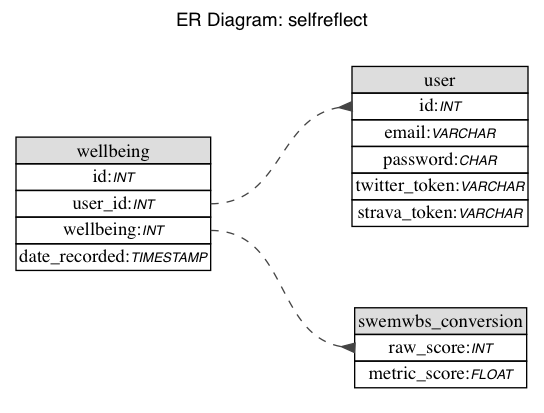
\includegraphics[width=0.8\textwidth]{i/selfreflectdb.png}
\label{fig:dberd}
\end{figure}

\newpage
This shows each of the tables, the columns in them, the types of each of these columns, and the relationships between tables.

\subsection{User Table}
This table includes:
\begin{itemize}
\item id: the primary key for the table. This is a unique identifier for each entry in the table, and is also a foreign key in the wellbeing table.
\item email: the email of the user.
\item password: the \emph{hashed} password of the user.
\item twitter\textunderscore token: the access token to access Twitter's API for this user.
\item strava\textunderscore token: the access token to access Strava's API for this user.
\end{itemize}

\subsection{Wellbeing Table}
This table includes:
\begin{itemize}
\item id: the primary key for the table. This is a unique identifier for each entry in the table.
\item user\textunderscore id: foreign key referencing the id column in the user table. Needed to map each wellbeing entry to a user. This has the added benefit of only allowing user ids that exist in the user table to be inserted into the wellbeing table.
\item wellbeing: foreign key referencing the raw\textunderscore score column in the swemwbs\textunderscore conversion table. This is the raw score, and has the added benefit of only allowing raw scores that are in the conversion to be inserted into the wellbeing table.
\item date\textunderscore recorded: timestamp field to store when the wellbeing was recorded.
\end{itemize}

\subsection{SWEMWBS Conversion Table}
This table is entirely static and will contain the SWEMWBS raw to metric score conversion table, as found in appendix \ref{swemwbsconversiontable}. This table includes:
\begin{itemize}
\item raw\textunderscore score: the primary key for the table. This is a the raw score in the SWEMWBS conversion table.
\item metric\textunderscore score: the metric score each raw score entry maps to.
\end{itemize}

\chapter{Implementation}
\section{Introduction}
This chapter will detail the implementation of the design discussed in the previous chapter. It will explain specific implementation details where necessary (where implementation is not trivial), and will detail where the implementation changed from the design and why. Code snippets and images will be included and referenced throughout to aid explanation.

\section{Mobile App}
The mobile app was developed using React Native, as discussed in the design section. Additionally, in order to reduce development time and avoid repeating work carried out by the software development community, an open source library called \enquote{Native Starter Kit} was used \parencite{nativestarterkit}. This library is a \enquote{starter kit that you can install on the fly to get the basic plumbing of React Native}, with the principle that there is \enquote{no need of reinventing the wheel} \parencite{nativestarterkit}. This provided a base app from which to build the SelfReflect mobile app, which included basic navigation, \enquote{boilerplate} code that is standard to any React Native project, and some example screens that could be adapted.

\subsection{Login}
The implemented login screen can be seen in Figure \ref{fig:mobileloginimpl}.

\begin{figure}[ht]
\centering
\caption{Mobile App Implemented Login Screen}
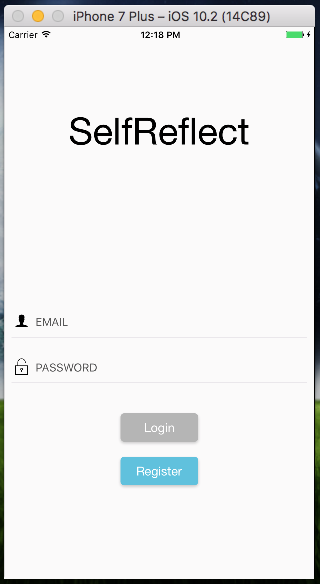
\includegraphics[width=0.3\textwidth]{i/mobileloginimpl.png}
\label{fig:mobileloginimpl}
\end{figure}

This is very similar to the wireframe in the design section (Figure \ref{fig:mobilelogin}) with some small styling improvements. The login page has two interesting pieces of functionality: input validation and the login itself.

\subsubsection{Login Input Validation}
Input validation is relatively simple. The login button is disabled unless the user provides a valid email, and some password (i.e. non empty). The function in the following code snippet returns true if both of these conditions are met:

\begin{lstlisting}
inputsValid() {
  return isValidEmail(this.state.email) && this.state.password
}
\end{lstlisting}

This does of course require some validation on the format of an email, hence the call to the isValidEmail function. Email validation is a topic that is debated regularly in web development, with some arguing for complex validation, and others arguing for simple validation with email verification. For this project, a very simple validation function was used. This simply checks the email matches a \emph{something@something.something} format, as shown in the following code snippet:

\begin{lstlisting}
const simpleEmailRegex = /^(.+)@(.+)\.(.+)$/

export default email => {
  return simpleEmailRegex.test(email)
}
\end{lstlisting}

The regular expression (or RegEx) in the above snippet is exactly the format previously described (\emph{something@something.something}).

Should either of the inputs fail validation, an error message will be displayed to the user, to inform the user which input is failing validation and why. This can be seen in Figure \ref{fig:mobileloginerror}.

\begin{figure}[ht]
\centering
\caption{Mobile App Implemented Login Screen Validation Error}
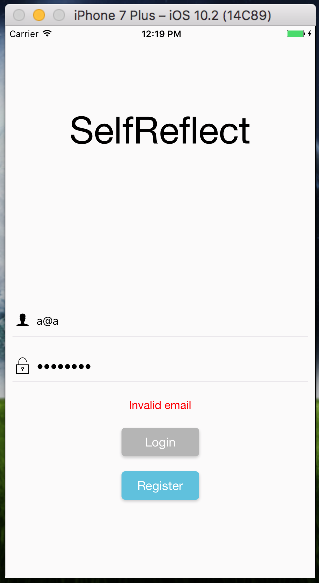
\includegraphics[width=0.3\textwidth]{i/mobileloginerror.png}
\label{fig:mobileloginerror}
\end{figure}

\subsubsection{Login}
When the user taps login, the email and password are sent to the SelfReflect API to check they are valid credentials. The code for posting user credentials to the server is shown in the following code snippet:
\begin{lstlisting}
login(onSuccess) {
  return fetch(apiUrl + '/v1/tokens', {
    method: 'POST',
    headers: {
      'Accept': 'application/json',
      'Content-Type': 'application/json',
    },
    body: JSON.stringify({
      email: this.state.email,
      password: this.state.password,
    })
  })
    .then(response => {
      ...
    })
}
\end{lstlisting}

This executes an AJAX request which posts the login credentials, in JSON format, to the SelfReflect API endpoint \emph{/v1/tokens}. Versioning was included in the API implementation, hence the \enquote{v1}, as will be discussed in section \ref{sec:apiimpl}.

Some code has been removed from the function in this snippet. The removed code simply handles whatever response the app gets from the server. If the credentials sent are valid, the mobile app will receive a success response code and an access token. It can then store this access token for subsequent requests, and execute the onSuccess function. This function will navigate the user to the \enquote{logged in} area of the app. If the credentials are invalid, the app will receive an error response code, and the login screen will display an \enquote{Invalid email or password} message, in exactly the same way as the \enquote{Invalid email} message in Figure \ref{fig:mobileloginerror}. It is possible the app will receive some other response from the server, if the database is down for example, in which case the mobile app will simply display \enquote{Something went wrong. Please try again later}.

\subsection{Register}
The register screen is very similar to the login screen. The implemented register page can be seen in Figure \ref{fig:mobileregisterimpl}.

Again, similar to the login screen, the register page does two main things: input validation and the register itself.

\begin{figure}[ht]
\centering
\caption{Mobile App Implemented Register Screen}
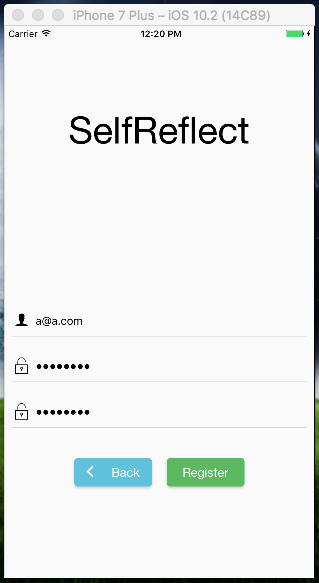
\includegraphics[width=0.3\textwidth]{i/mobileregisterimpl.png}
\label{fig:mobileregisterimpl}
\end{figure}

\subsubsection{Register Input Validation}
This is again very similar to the login input validation, with the additional check that the password and confirm password must match. The code to do this is seen in the following snippet:
\begin{lstlisting}
inputsValid() {
  return isValidEmail(this.state.email)
    && this.state.password
    && (this.state.password === this.state.confirm);
}
\end{lstlisting}
Again, like the login page, failed validation will result in the register button being disabled and an error message being displayed to the user, as seen in Figure \ref{fig:mobileregistererror}.

\begin{figure}[ht]
\centering
\caption{Mobile App Implemented Register Screen Validation Error}
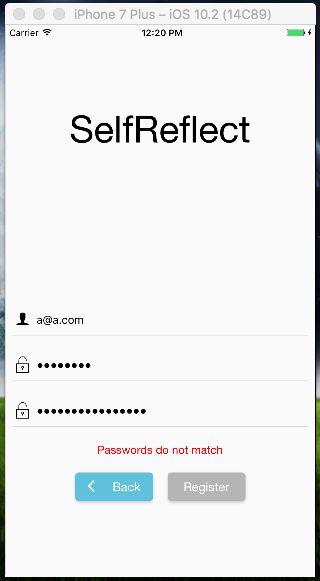
\includegraphics[width=0.3\textwidth]{i/mobileregistererror.png}
\label{fig:mobileregistererror}
\end{figure}

\newpage
\subsubsection{Register}
This is again similar to the functionality for login, but of course accesses a different endpoint of the SelfReflect API, in this case \emph{/v1/users}. The code to register a user is shown below:
\begin{lstlisting}
register(onSuccess) {
  return fetch(apiUrl + '/v1/users', {
    method: 'POST',
    headers: {
      'Accept': 'application/json',
      'Content-Type': 'application/json',
    },
    body: JSON.stringify({
      email: this.state.email,
      password: this.state.password,
    })
  })
    .then(response => {
      ...
    })
}
\end{lstlisting}

This is clearly extremely similar to the login code. This will become a similar theme throughout this entire chapter, and is due to the API having been buillt in a RESTful way; all accesses tend to follow a similar, \enquote{uniform} pattern. For this reason not all of these API accesses will be included in code snippets; they will simply be described, as they are almost all fairly similar. Again, the success and error codes are handled in much the same way, and displayed to the user if necessary, such as for \enquote{Email already exists} responses. In the case of register, the onSuccess function will navigate back to the login page, so the user can log in with their newly created account.

\subsection{Home}
Once the user has logged in successfully, they will be navigated to the home screen, as seen in Figure \ref{fig:mobilehomeimpl}. For demonstration purposes, a test account with some existing wellbeing recordings was used.

\begin{figure}[ht]
\centering
\caption{Mobile App Implemented Home Screen}
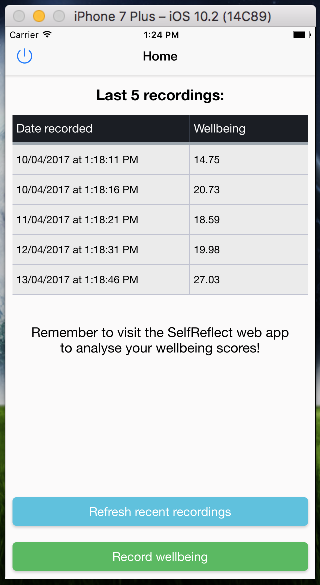
\includegraphics[width=0.3\textwidth]{i/mobilehomeimpl.png}
\label{fig:mobilehomeimpl}
\end{figure}

This is similar to the wireframe for the home screen in the design section (Figure \ref{fig:mobilehome}), with a few changes. Most of these changes are styling and other small changes, but one is the addition of the \enquote{Refresh recent recordings} button. The button simply repopulates the recent recordings table. During implementation it was discovered that if the user recorded their wellbeing on the web app, the only way to get the table in the mobile app to refresh would be to exit and reload the app, which was not very \enquote{user-friendly}. Adding this button solved this issue at little extra cost, as all the functionality to populate the table was already implemented.

The logout button (the \enquote{power} button in the top left) simply navigates the user back to the login screen, which they then cannot get through without logging in again. The population of the last five recent recordings table however is a little more complicated.

\subsubsection{Last 5 Recordings Table}
The code to fetch a user's last five recordings is not vastly different to the API accesses in the login and register pages. However, this is now accessing user data, so the token (obtained at successful login) must be sent with the request. The code to fetch this data is seen below:

\begin{lstlisting}
fetchHistory(id, token) {
  return fetch(apiUrl + '/v1/users/' + id + '/wellbeings?limit=5', {
    method: 'GET',
    headers: {
      'Accept': 'application/json',
      'Content-Type': 'application/json',
      'Authorization': 'Bearer ' + token
    }
  })
    .then(response => {
      ...
    })
\end{lstlisting}

This limits the number of recent wellbeings the API responds with to five, as there are only five rows in the table. It also passes the token in the \emph{Authorization} header of the request. This is how all restricted API endpoints are accessed by SelfReflect clients, and will again be seen throughout this chapter. The response is then stored in state, allowing the table to be populated.

The table is a simple grid of rows and columns. To generate the table, the app processes this stored data, by formatting dates and sorting entries in ascending date order. It then simply maps over the processed wellbeing entries, and produces a row for each entry with two columns: one for date recorded and one for wellbeing. The code to do this can be seen below:
\begin{lstlisting}
{this.props.history.map((wellbeing, i) =>
  <Row key={i} style={styles.row}>
    <Col style={styles.leftCol} size={3}>
      <Text style={styles.text}>{wellbeing.date_recorded}</Text>
    </Col>
    <Col style={styles.rightCol} size={2}>
      <Text style={styles.text}>{wellbeing.wellbeing}</Text>
    </Col>
 </Row>
)}
\end{lstlisting}

This syntax is \enquote{JSX}. JSX is \enquote{a preprocessor step that adds XML syntax to JavaScript}, and is used to make \enquote{React a lot more elegant} \parencite{jsx}. It essentially allows code that looks similar to HTML to be written within JavaScript, producing more readable and intuitive code.

\subsection{SWEMWBS Questions}
Tapping the record wellbeing button will navigate users to the SWEMWBS questions. This is implemented almost exactly as in the design chapter (Figure \ref{fig:mobilequestion}), and can be seen in Figure \ref{fig:mobilequestionimpl}.

\begin{figure}[ht]
\centering
\caption{Mobile App Implemented SWEMWBS Question Screen}
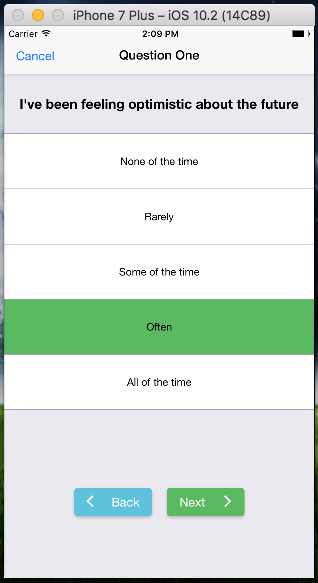
\includegraphics[width=0.3\textwidth]{i/mobilequestionimpl.png}
\label{fig:mobilequestionimpl}
\end{figure}

The next button on each question screen is disabled until an answer is selected. One change that was made from the design is the inclusion of the cancel button. This was implemented instead of the logout button, so that if a user wanted to cancel and go back to the home screen, they can do so without pressing back lots of times, or without having to log out and in again.

The last question includes a submit button instead of a next button, which simply sums the scores to each of the answers (where \enquote{None of the time} has a score of 1, \enquote{Rarely} has a score of 2 etc.), computes the date and time of submission, and posts these to the \emph{/v1/users/:id/wellbeings} endpoint, where \emph{:id} is the user ID obtained on successful login. This code has not been included here as it is very similar to the API accesses described in previous sections. It again handles both successful and error responses from the server, by either navigating the user back to the home page on success, or displaying an error message on error.

If successful, this also automatically updates the state that the recent recordings table (on the home screen) is generated from with the new wellbeing entry, based on the API response. This allows the user to instantly see that their wellbeing was recorded successfully.

\subsection{Documentation}
Documentation was written for the mobile app that includes a short description of SelfReflect and the SelfReflect mobile app, as well as instructions on how to install, set up and run the mobile app for local development and testing. This documentation can be seen in appendix \ref{app:mobiledocs}.

\section{Web App}
Then web app was developed using the various technologies discussed in the design section (section \ref{sec:webappdesign}), including React, Redux and Skeleton CSS.

\subsection{React and the Redux Store}
Before the implementation of each page in the web app is described, the implementation of persistent state and the Redux store will be described. When developing a React application, the entire application is rendered based on state. Changes to the app, based on user input, are then simply changes to the state. React notices these changes, computes what will change due to this new state, then updates with the \enquote{document object model}, or DOM, with these changes.

Redux is a tool and development methodology for managing state in a React application, by creating a \enquote{store} that holds state. Large applications can become confusing due to a huge amount of state, so Redux helps to organise state in a uniform, modular way. Redux requires \enquote{reducers} to be passed when creating the store. These define all possible ways to update the state in the store. This limits the ways state can be accessed/updated, and is one of the main ways Redux helps to arrange state and updates to state, in a uniform and organised way.

\subsubsection{Initialising State}
Another feature Redux provides is the ability to initialise the store with some pre-loaded state. This is how persisted state was implemented in the web app. The following code does this:
\begin{lstlisting}
export const loadState = () => {
  try {
    const state = localStorage.getItem('state')

    if (state === null) {
      return
    }

    return JSON.parse(state)
  } catch (_) {
    return
  }
}

...

const persistedState = loadState()

const store = createStore(reducers, persistedState)

\end{lstlisting}
This loads the state from \enquote{HTML Local Storage} \parencite{htmllocalstorage}, and initialises the store with this state. The user and token are stored in browser memory (HTML Local Storage), then loaded when the web app is loaded. This persists user's login, as long as the token is not expired.

\newpage
\subsubsection{Persisting State}
In order to store state in HTML Local Storage, another Redux feature was used. Redux allows attaching of \enquote{listeners} to the store. These are callback functions that are called every time the state changes. In order to store the user and token, the following code attaches a listener to the store:
\begin{lstlisting}
export const persistState = state => {
  try {
    const serializedState = JSON.stringify(state)

    return localStorage.setItem('state', serializedState)
  } catch (_) {
    return
  }
}

...

store.subscribe(() => {
  const user = store.getState().user
  const token = store.getState().token

  // If no user id in new state, user has logged out, so clear persisted state
  if (!user.id) {
    return clearState()
  }

  if (user.isLoading) {
    return
  }

  if (!persistedState) {
    return persistState({ user, token })
  }

  // If nothing changed, do nothing
  if (equals(user, persistedState.user) &&
      equals(token, persistedState.token)) {
    return
  }

  persistState({ user, token })
})
\end{lstlisting}

This code is invoked whenever the state changes in the store. It checks to see if the user or token has changed in that state update, and persists these in HTML Local Storage if either of these have changed.

\subsubsection{Token Refresh}
In order to refresh tokens that come close to expiry, the following code was added to add another listener to the Redux store:
\begin{lstlisting}
export const refreshToken = (dispatch, token) => {
  return fetch(api + '/v1/tokens', {
    method: 'PUT',
    headers: {
      'Accept': 'application/json',
      'Content-Type': 'application/json',
      'Authorization': 'Bearer ' + token.value
    }
  })
    .then(response => {
      // Some error
      if (response.status !== 200) {
        return
      }

      // Success
      return response.json()
        .then(json => {
          dispatch(setToken({ value: json.token, exp: json.exp }))
        })
    })
    .catch(_ => {
      return
    })
}

...

store.subscribe(throttle(300000, () => {
  const token = store.getState().token
  const nowInSeconds = Math.floor(Date.now() / 1000)

  // If no token, or if token going to expire in more than an hour, do nothing
  if (!token.value || (token.exp - 3600 > nowInSeconds)) {
    return
  }

  refreshToken(store.dispatch, token)
}))
\end{lstlisting}

This checks to see if the token exists and is going to expire in less than an hour. If these conditions are met, it refresheds the token using a PUT request to the \emph{/v1/tokens} endpoint of the SelfReflect API. One other thing of note in this code snippet is that the function is \enquote{throttled}. This limits how often this function can be called, so as not to slow down the application or add unnecessary load on the server. In this case the function is throttled to once every 300 seconds, or five minutes.

\subsubsection{Update User Information}
In order to ensure the information about the currently logged in user stays as \enquote{up-to-date} as possible, a listener was added that regularly updates the user's information. This is so that if some other client was used to edit the email of a user, for example, this would be updated and represented in the SelfReflect web app. The code to add this listener is shown below:

\begin{lstlisting}
const throttledFetchUser = throttle(300000, (dispatch, userId, token) => {
  fetchUser(dispatch, userId, token)
})

...

store.subscribe(() => {
  const user = store.getState().user
  const token = store.getState().token

  // If already loading, user not logged in, or if token invalid, do nothing
  if (user.isLoading || !user.id || !validateToken(token)) {
    return
  }

  // If first time fetching, do not throttle
  if (!user.email) {
    return fetchUser(store.dispatch, user.id, token)
  }

  throttledFetchUser(store.dispatch, user.id, token)
})
\end{lstlisting}

The fetchUser function (not shown) simply fetches the user's information by sending a GET request to the \emph{/v1/users/:id}. It then updates the user's information in the Redux store state. This is again throttled, but in a slightly different way. The function needs to not be throttled if the user has not been fetched yet, so both the throttled and original versions of the \emph{fetchUser} function are required.

\subsection{Home}
The first screen the user sees when loading the web app is the home screen, which can be seen in Figure \ref{fig:webhomeimpl}.

\begin{figure}[ht]
\centering
\caption{Web App Implemented Home Screen}
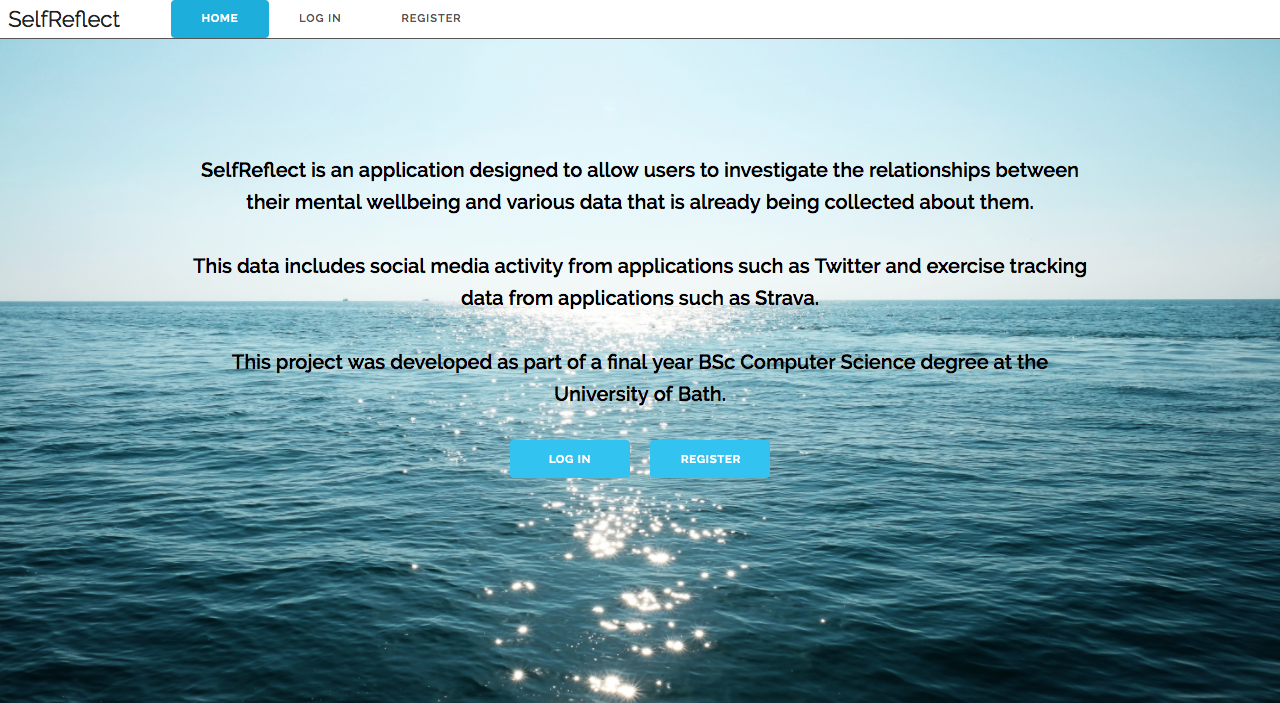
\includegraphics[width=\textwidth]{i/webhomeimpl.png}
\label{fig:webhomeimpl}
\end{figure}

This includes a short description of the SelfReflect system, and buttons to navigate to the log in and register screen. It also includes a background image which was added to make the website a little more interesting and professional. This screen is slightly different depending on whether the user is logged in or not, the only difference being the log in and register buttons are not present when the user is logged in.

\subsection{Login}
Clicking the log in button either on the home page or in the navigation bar will navigate the user to the login screen, as can be seen in Figure \ref{fig:webloginimpl}.

\begin{figure}[ht]
\centering
\caption{Web App Implemented Login Screen}
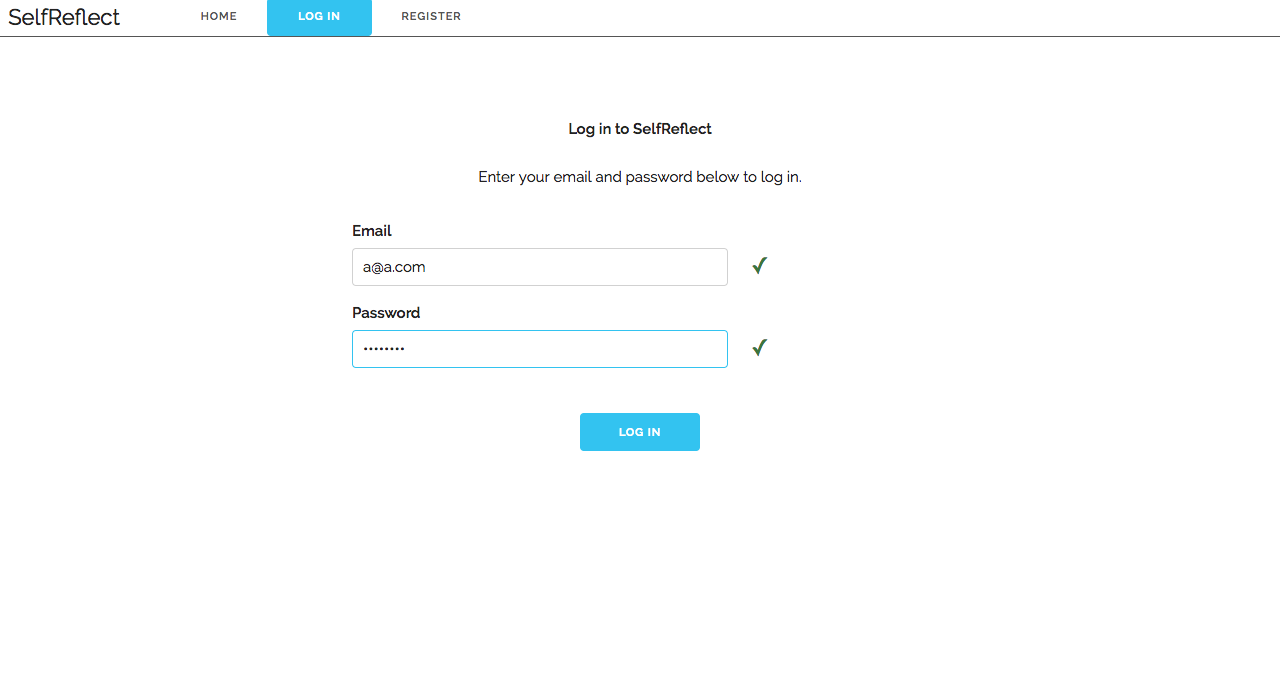
\includegraphics[width=.8\textwidth]{i/webloginimpl.png}
\label{fig:webloginimpl}
\end{figure}

Much like the mobile app, the web app login page handles the same two functions: input validation and login.

\newpage
\subsubsection{Login Input Validation}
If input validation is failed, the log in button will do nothing. Input validation for the web app login form is done in exactly the same way as it was in the mobile app. For this reason, the code has not been included here as it is not significantly different to that of the mobile app. The login page with failed input validation can be seen in Figure \ref{fig:webloginerror}.

\begin{figure}[ht]
\centering
\caption{Web App Implemented Login Screen Validation Error}
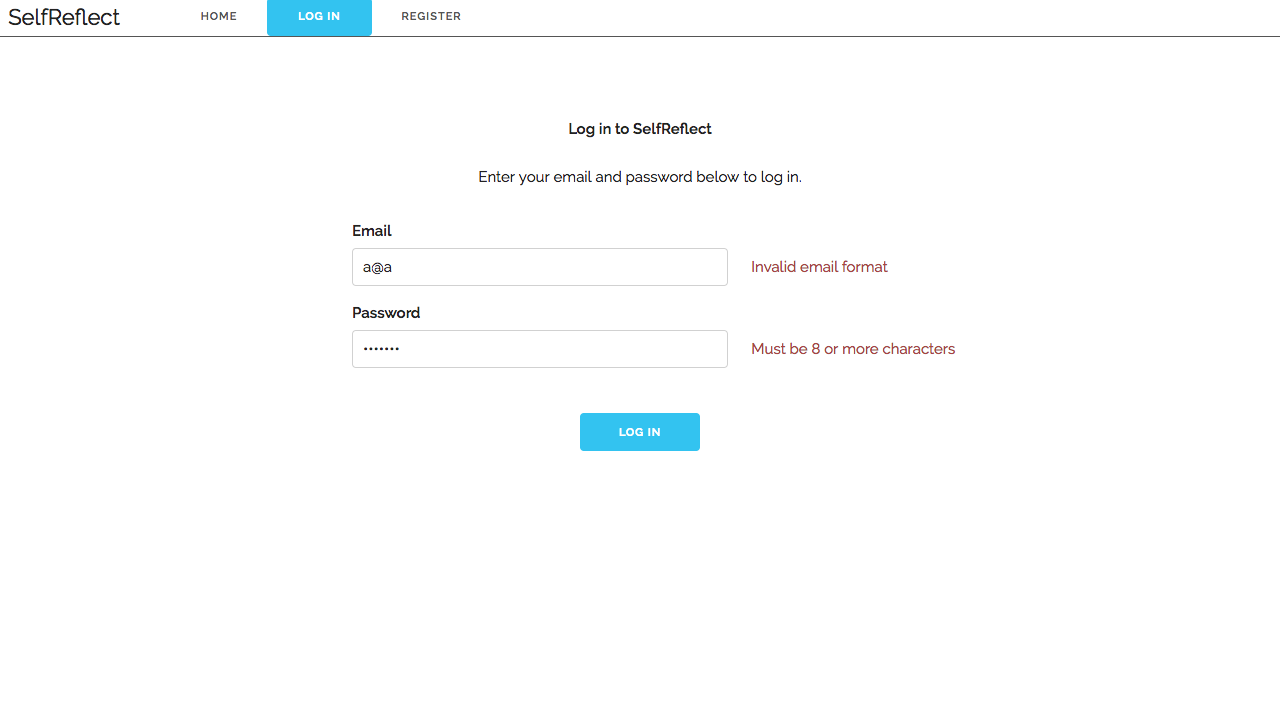
\includegraphics[width=.8\textwidth]{i/webloginerror.png}
\label{fig:webloginerror}
\end{figure}

\subsubsection{Login}
The login functionality of the web app is almost identical to the login functionality of the mobile app. For this reason the code has not been included here. It is almost identical, except it handles responses (success/error) with Redux. After a successful login, the user is navigated to the guide page (see section \ref{subsec:guide}).

\subsection{Register}
Clicking the register button either on the home page or in the navigation bar will navigate the user to the register screen, as can be seen in Figure \ref{fig:webregisterimpl}.

\begin{figure}[ht]
\centering
\caption{Web App Implemented Register Screen}
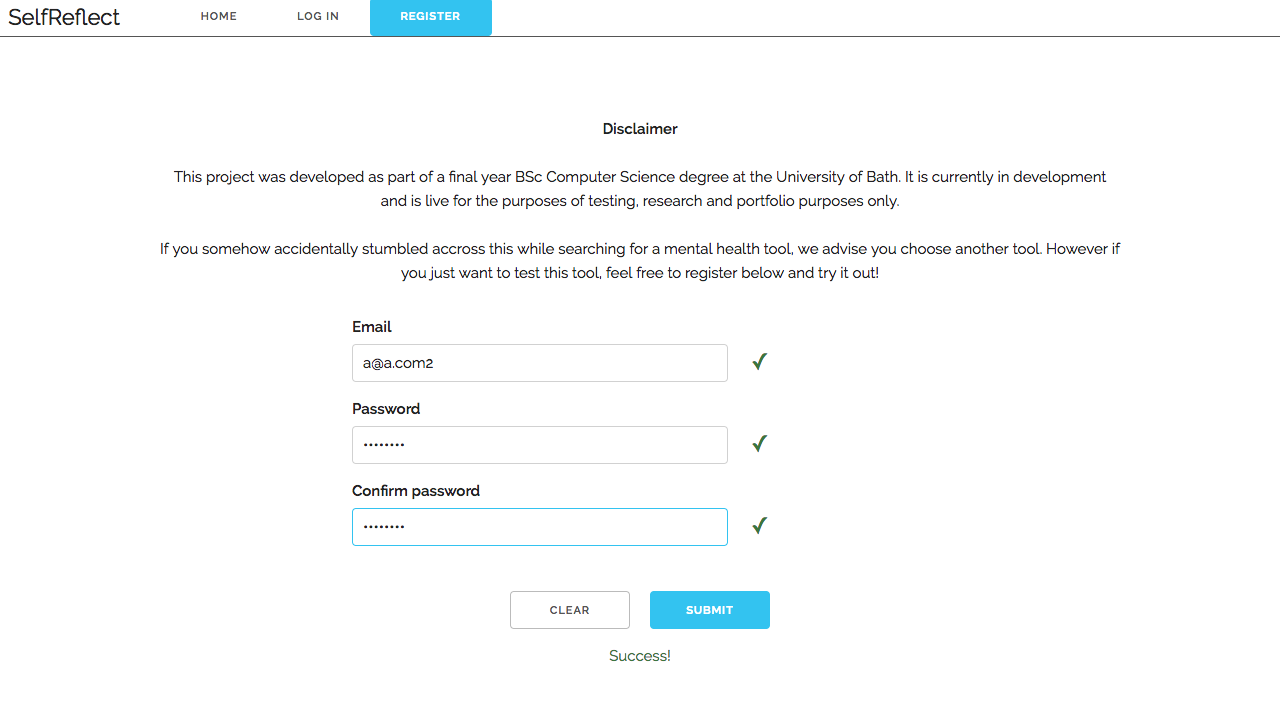
\includegraphics[width=\textwidth]{i/webregisterimpl.png}
\label{fig:webregisterimpl}
\end{figure}

Again the web app register page handles two functions: input validation and register. There are also two key changes to the implemented register page. Firstly, a disclaimer has been added. The web app was hosted live temporarily during this project for the purposes of testing, so this disclaimer was included in case someone accidentally found the live site. This is unlikely but was included anyway to be safe. The second change is the inclusion of the clear button. This allows users to quickly clear all inputs, should they make a mistake or wish to register another account for some reason.

\newpage
\subsubsection{Register Input Validation}
This is again exactly the same as the mobile app. The register page with failed input validation can be seen in Figure \ref{fig:webregistererror}.

\begin{figure}[ht]
\centering
\caption{Web App Implemented Register Screen Validation Error}
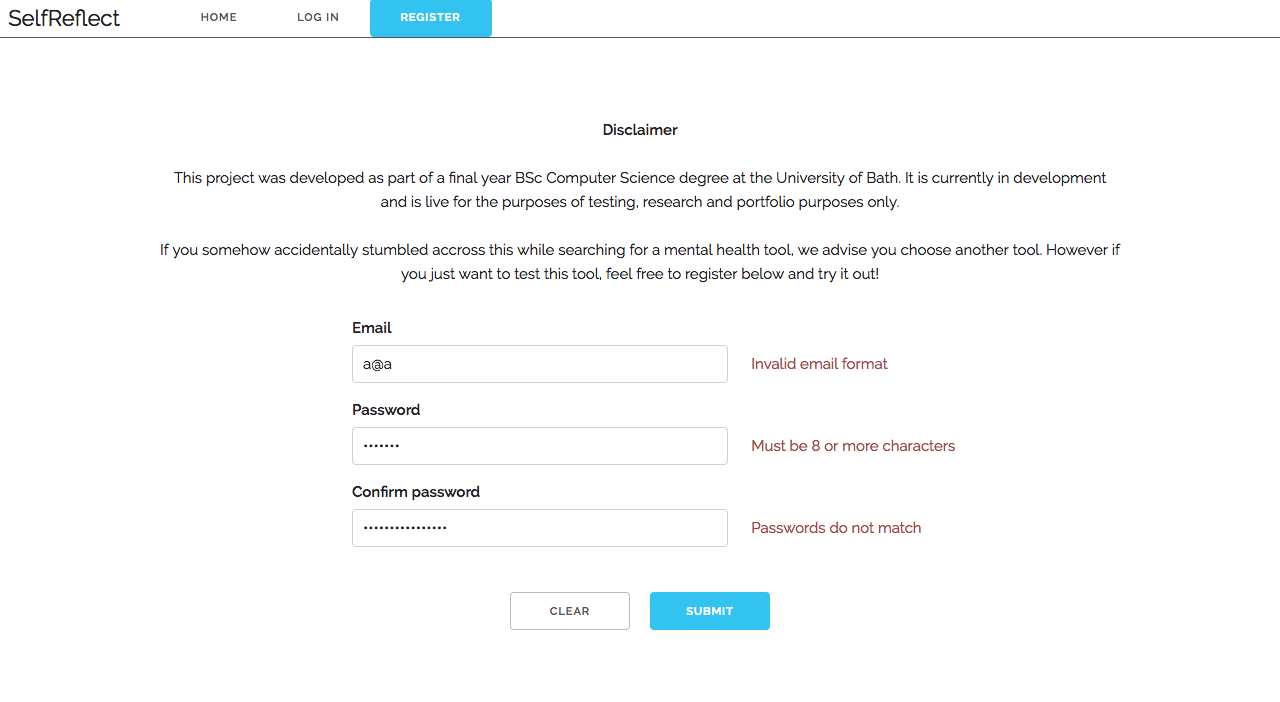
\includegraphics[width=\textwidth]{i/webregistererror.png}
\label{fig:webregistererror}
\end{figure}


\subsubsection{Register}
Again, the register functionality is almost identical to that of the mobile app, so does not need to be described again. After a successful register, a success message appears to indicate the account has been created.

\subsection{Guide} \label{subsec:guide}
The guide page was implemented almost exactly like the wireframe in the design section (Figure \ref{fig:webguide}), but with some styling improvements. This can be seen in Figure \ref{fig:webguideimpl}.

\begin{figure}[ht]
\centering
\caption{Web App Implemented Guide Screen}
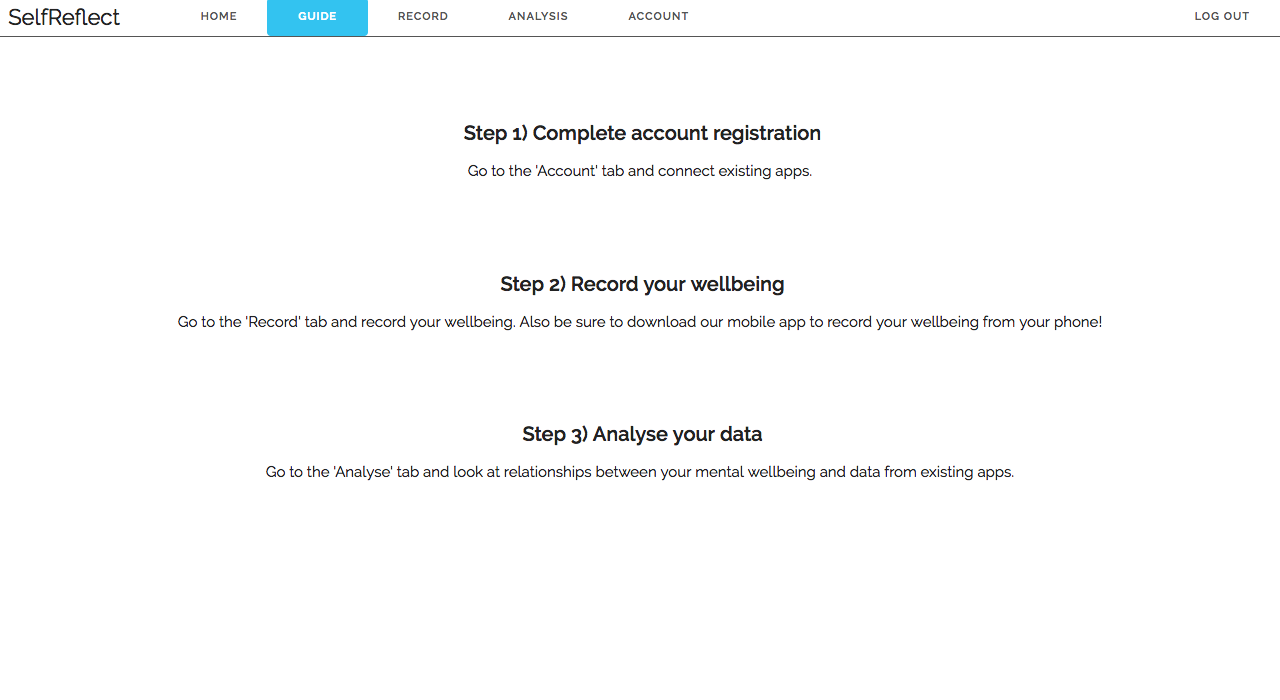
\includegraphics[width=\textwidth]{i/webguideimpl.png}
\label{fig:webguideimpl}
\end{figure}

\newpage
As Figure \ref{fig:webguideimpl} shows, the navigation bar is different if the user is logged in. Being logged in gives access to the guide, analysis and account pages. It also adds the log out button.

As the entire web app is rendered and updated based on state, the log out button simply clears the relevant state. This is done with the following code:
\begin{lstlisting}
logout: () => {
  dispatch(resetUser())
  dispatch(resetToken())

  dispatch(setSelectedTab('home'))
}
\end{lstlisting}

This clears all state relevant to the user, clears the access token from state, and navigates the user back to the home page. This would, due to the listener described earlier, also clear the persisted state in HTML Local Storage. The user would therefore have to log in again to be able to access the \enquote{logged in} areas of the application.

\subsection{Record/SWEMWBS Questionnaire}
The SWEMWBS questionnaire can be found on the record page. This is almost identical to the wireframe in the design section (Figure \ref{fig:webrecord}). The top of the record page can be seen in Figure \ref{fig:webrecordimpltop} and the bottom in Figure \ref{fig:webrecordimplbottom}.

\begin{figure}[ht]
\centering
\caption{Web App Implemented Record Screen Top of Page}
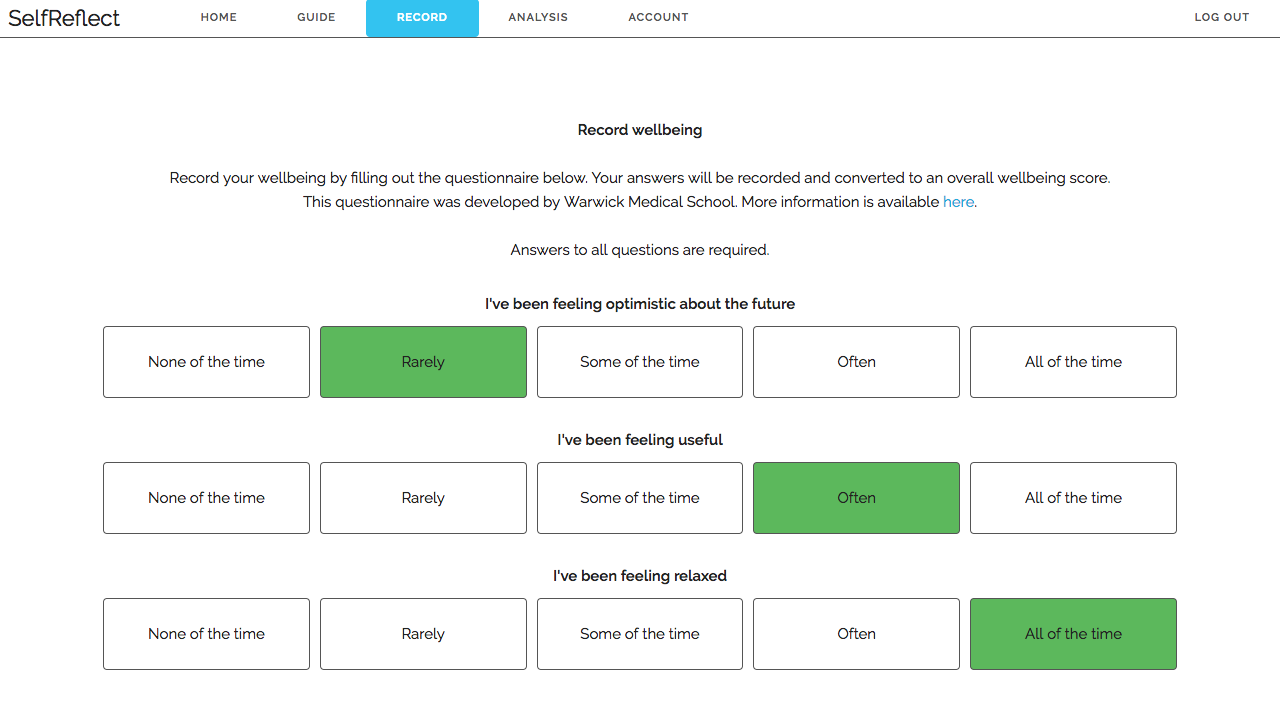
\includegraphics[width=.75\textwidth]{i/webrecordimpltop.png}
\label{fig:webrecordimpltop}
\end{figure}

\begin{figure}[ht]
\centering
\caption{Web App Implemented Record Screen Bottom of Page}
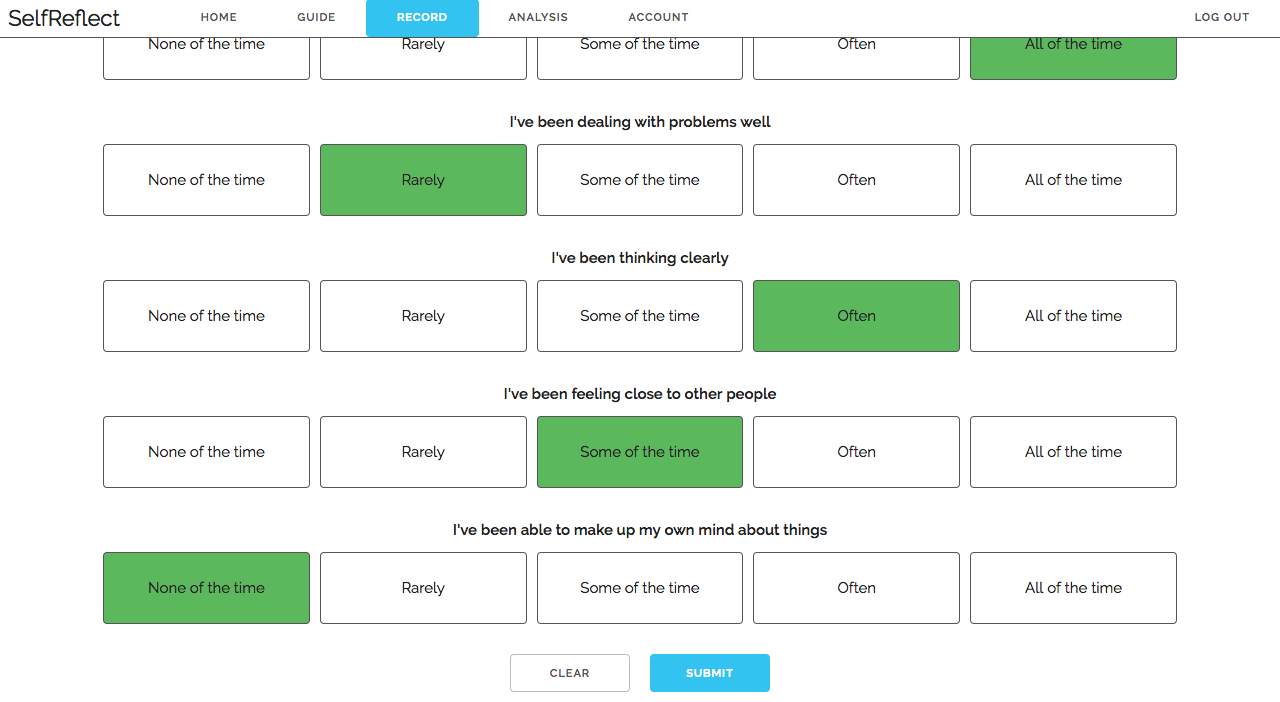
\includegraphics[width=.75\textwidth]{i/webrecordimplbottom.png}
\label{fig:webrecordimplbottom}
\end{figure}

\newpage
The only significant change to the design is the addition of the clear button which, much like the register page, clears all of the answers to the questionnaire.

The submit button is disabled until all the questions are answered. When it is enabled and pressed, the sum of the answers and the current date and time are calculated. These are then submitted to the SelfReflect API in exactly the same way as the questions in the mobile app. The user is then presented with a success message and the answers are cleared.

\subsection{Account}
The account page is divided into two areas: account management and connect existing apps. An overall view of the page can be seen in Figure \ref{fig:webaccountimpl}.

\begin{figure}[ht]
\centering
\caption{Web App Implemented Account Screen}
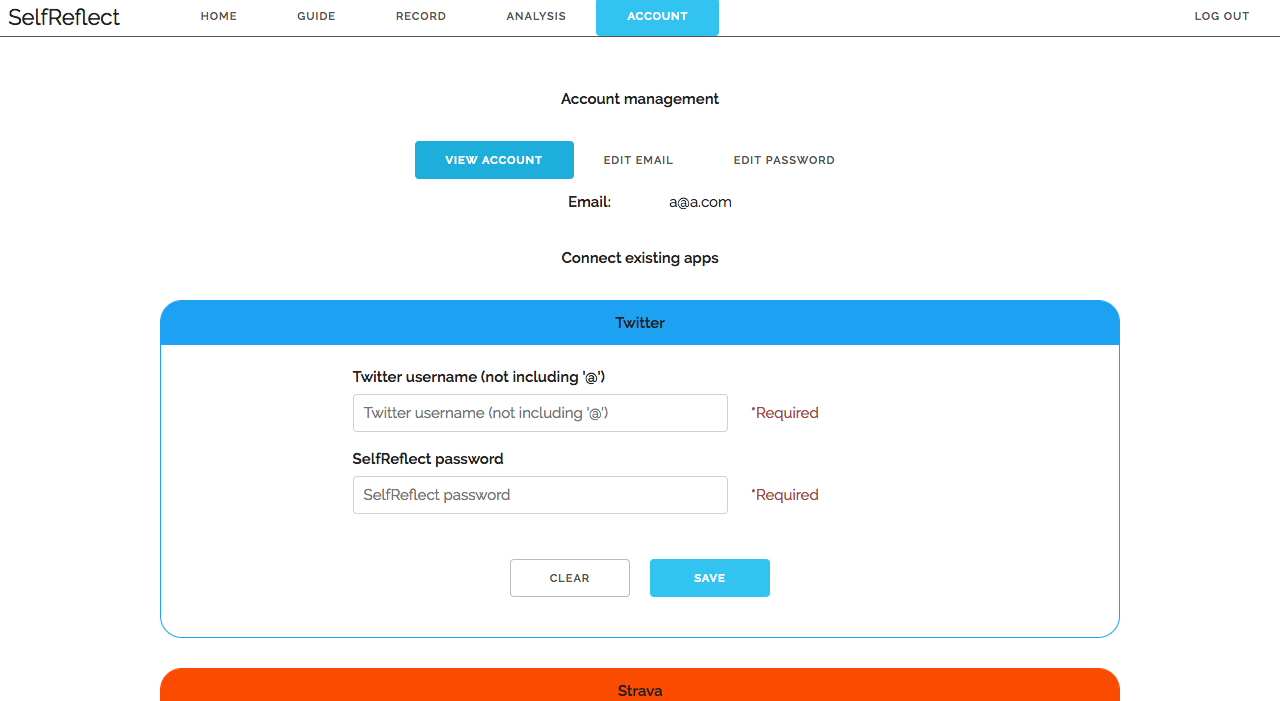
\includegraphics[width=.8\textwidth]{i/webaccountimpltop.png}

\includegraphics[width=.8\textwidth]{i/webaccountimplbottom.png}
\label{fig:webaccountimpl}
\end{figure}

\subsubsection{Account Management}
The first section of the account page deals with account management. This section contains three \enquote{tabs}: view account, edit email and edit password. These can be seen in Figure \ref{fig:webaccounttabs}.

\begin{figure}[ht]
\centering
\caption{Web App Implemented Account Management Tabs}

\includegraphics[width=.48\textwidth]{i/webaccountviewtab.png} \\
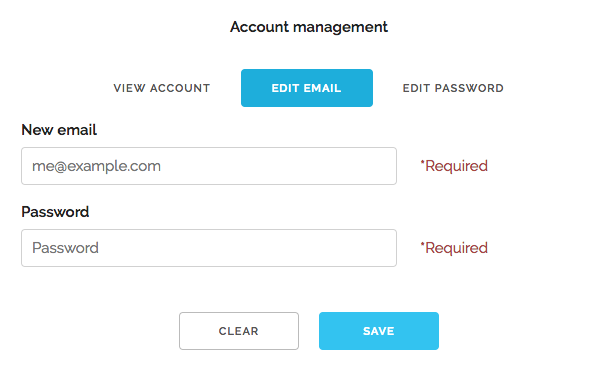
\includegraphics[width=.48\textwidth]{i/webaccountemailtab.png} \hfill
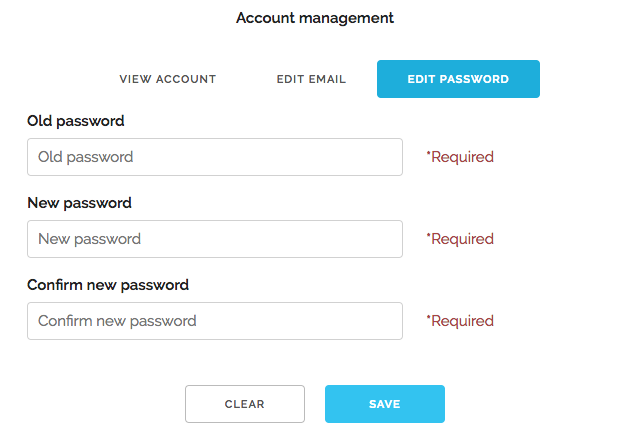
\includegraphics[width=.48\textwidth]{i/webaccountpasswordtab.png}
\label{fig:webaccounttabs}
\end{figure}

\newpage
A change made from the design of this page (in Figure \ref{fig:webaccount}) was the addition of the view account tab. This was originally not included, but automatically displaying either of the edit forms seemed strange from a user experience point of view. The user may simply want to view their details rather than edit them. This also provides some feedback for the user if they change their email, as the view account tab will automatically be updated to their new email.

The edit email and edit password forms are relatively simple. They use the same validation rules as the register page, require the current password to be provided for security reasons, and send a PUT request to the \emph{/v1/users/:id} endpoint of the SelfReflect API. The body of this request contains the full original user, with either the \emph{email} or the \emph{newPassword} field changed, for edit email and edit password respectively. See section \ref{sec:apiimplusers} for further details on this.

Both of these forms contain a clear button, which work in exactly the same way as other clear buttons described in this chapter. They simply clear the inputs of that form. Both forms also handle successful and error responses from the server, and report these to the user.

\subsubsection{Connect Existing Apps} \label{subsec:webconnectapis}
The second area of this page is the connect existing apps area. This allows the user to connect Twitter and Strava to their SelfReflect account. The colours for the boxes surrounding the Twitter and Strava areas are taken from the respective logos for each of the applications.

\paragraph{Twitter} This changed quite substantially from the design of the account page (Figure \ref{fig:webaccount}). The reason for this relates to both the web app and the API. During implementation it was found that Twitter provide \enquote{application-only authentication} \parencite{twitterapponly}. This allows an application to access certain endpoints of the Twitter API by authenticating itself, rather than the user. It also provides a higher rate limit for these endpoints.

The details of the application only authentication will be discussed in section \ref{sec:apiconnecttwitter}, but one of these endpoints allows the SelfReflect API to fetch user timelines (i.e. recent tweets). For this reason Twitter does not need to be fully connected; SelfReflect simply needs the user's Twitter username to be able to fetch their tweets. This is therefore a \enquote{user level} update, so is implemented in almost exactly the same way as the edit email and edit password forms. The current password is required for security, and a PUT request is sent to \emph{/v1/users/:id}, with the \emph{twitter\textunderscore username} field changed.

The form itself contains elements discussed before; a clear button, handling of success and error responses, and basic twitter username validation. This validation is handled by the following code, which as the comment states, simply checks the username is between one and fifteen characters, and contains only letters, numbers and underscores:
\begin{lstlisting}
// Letters, numbers and underscores, and 1-15 characters
export default twitter_username => (
  twitter_username && /^[a-zA-Z0-9_]{1,15}$/.test(twitter_username)
)
\end{lstlisting}

\paragraph{Strava} Strava does not provide application only authentication, and so must be fully connected to allow the SelfReflect to fetch the user's exercise data. This is a fairly complicated process that was made more complicated by the fact the the SelfReflect web app is a \enquote{one page} app. The following stages are required to connect a user's Strava account to any application:
\begin{enumerate}
\item Direct the user to Strava's authorisation page. If the user accepts, Strava will respond with a code.
\item Exchange this code for a Strava access token.
\item Use this access token in subsequent requests.
\end{enumerate}

\newpage
The first of these stages is handled by the following code in the SelfReflect web app:
\begin{lstlisting}
import { authURL, clientId, redirectUri } from '../../../../config/strava'

const onClickConnect = (userId, tokenValue) => () => {
  const state = { userId, tokenValue }

  window.open(authURL +
    '?client_id=' + clientId +
    '&state=' + JSON.stringify(state) +
    '&response_type=code' +
    '&redirect_uri=' + redirectUri
  )
}
\end{lstlisting}

This directs the user to the Strava authorisation page. It also provides two parameters of note:
\begin{enumerate}
\item \emph{state}. This is extremely important for stage 2 of connecting strava. It allows some state to be passed to Strava's authorization page, which is automatically passed back (unmodified) after the user accepts authorisation.
\item \emph{redirect\textunderscore uri}. This is where Strava will direct the user, and hence pass the code and state to, after the user accepts authorisation. This is the reason SelfReflect being a one page application caused issues when connecting Strava. The web app originally only had one page, meaning there was no page to redirect to that would be able to handle the Strava authorisation. To handle this, another page had to be added to the web app. This is accessible at \emph{/connectStrava} on the web app.
\end{enumerate}

This page handles part of stage 2 of connecting a user's Strava account. When the page is loaded, the GET parameters (state and code) are pulled from the address bar using the following code:
\begin{lstlisting}
const getParams = parse(window.location.search)
const state = JSON.parse(getParams.state)
\end{lstlisting}

The page then simply sends the code to the SelfReflect API (using the userId and the SelfReflect token, as is required by the SelfReflect API), which exchanges the code for a Strava access token and stores it in the SelfReflect database against that user. The page gives user feedback on the progress of connecting Strava as this happens, as shown in Figure \ref{fig:webstravaloading} and Figure \ref{fig:webstravasuccess}.

\begin{figure}[ht]
\centering
\caption{Web App Implemented Connect Strava Screen Loading Message}

\includegraphics[width=.75\textwidth]{i/webstravaloading.png}
\label{fig:webstravaloading}
\end{figure}

\begin{figure}[ht]
\centering
\caption{Web App Implemented Connect Strava Screen Success Message}

\includegraphics[width=.75\textwidth]{i/webstravasuccess.png}
\label{fig:webstravasuccess}
\end{figure}

\subsection{Analysis}
The final page of the web app is the analysis page, which includes the visualisations. This page can be seen in Figure \ref{fig:webanalysisimpl}.

\begin{figure}[ht]
\centering
\caption{Web App Implemented Analysis Screen}
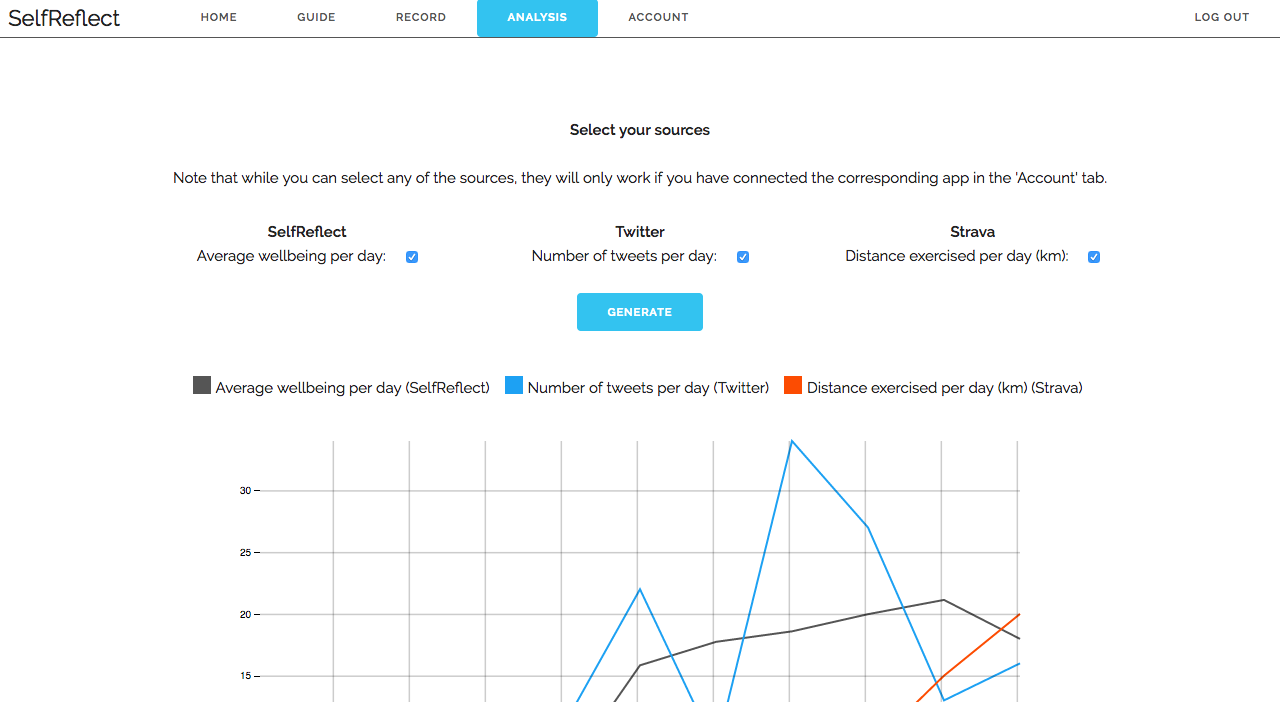
\includegraphics[width=\textwidth]{i/webanalysisimpl.png}
\label{fig:webanalysisimpl}
\end{figure}

This is much like the design for this page (Figure \ref{fig:webanalysis}). The user can select which sources they wish to build the visualisation from, then press generate. There are three key aspects to generating the graph:
\begin{enumerate}
\item Fetching the data.
\item Formatting the data.
\item Building the graph with the data.
\end{enumerate}

\subsubsection{Fetching the Data}
The data is fetched via the SelfReflect API. Each source requires a separate request, so a system was devised where functions do the following:
\begin{itemize}
\item Take some input data.
\item If the source for this function is selected, fetch the data for that source.
\item Merge the input data and fetched data. If fetched data is nothing (if source is not selected), this will just result in the input data.
\item Pass this merged data as input data to the next function in the \enquote{chain}.
\end{itemize}
This is a \enquote{functional} way of programming and allows the functions to be chained, as in the following code:
\begin{lstlisting}
const sortByDate = sortBy(prop('timestamp'))

const isWellbeing = sources.averageWellbeingPerDay
const isNumTweets = sources.numTweetsPerDay
const isDistance = sources.distanceExercisedPerDay

return fetchAverageWellbeingPerDay(isWellbeing, [], userId, token, data => {
  fetchNumTweetsPerDay(isNumTweets, data, userId, token, data => {
    fetchDistanceExercisedPerDay(isDistance, data, userId, token, data => {
      data = sortByDate(data)

      dispatch(updateIsLoading(false))

      dispatch(updateGraphData(data))
    })
  })
})
\end{lstlisting}

The result of this is that if extra sources are added in the future, it would be relatively easy to add them as an extra function in this chain. This simply then sorts the data by date, which is a unix timestamp, and updates this data in the state of the application, which the graph can then be built from. Note that these fetch functions also handle the formatting of the data.

\subsubsection{Formatting the Data}
Data is received from the SelfReflect API in its raw format, and it extremely unlikely that any two sources will return data in the same or even compatible ways. In the case of SelfReflect, Twitter and Strava this is true; three entirely different representations are used. Plus, the open source software used to generate the graph requires the data be provided in a very specific format.

In order to do this, raw data that is received from the SelfReflect API is processed after it is received and is converted into a consistent format. This involves converting all dates to unix timestamps, and merging data from multiple sources that happen to be from the same day. This allows multiple series to be plotted on the same graph. The code has not been included for this as it is large and repetitive, but it essentially sorts dates and data so that one set of merged data is produced that can be passed directly to the graph. An example of this merged data format would be:
\begin{lstlisting}
[
  {
    "timestamp":1492041600000,
    "totalWellbeing":42.269999999999996,
    "numWellbeings":2,
    "averageWellbeing":21.134999999999998,
    "numTweets":13,
    "distanceExercised":15
  },
  {
    ...
  },
  ...
]
\end{lstlisting}
The calculation of distance exercised and number of tweets is straightforward. For events on a repeated day, the value of that event is just added to the current total. The average wellbeing however is a little more complicated. This requires the \emph{totalWellbeing} and \emph{numWellbeings} to be updated throughout. Once all the data had been processed, an extra iteration is carried out in which the average wellbeing for each day is calculated, by dividing the total wellbeing on that day by the number of wellbeing recordings on that day.

\subsubsection{Building the Graph}
Once the data is processed into this format and updated in state, generating the graph is easy. The only things left to do are define the series of the chart, and actually generate the graph. In order to define the chart series, the selected sources are mapped over, and an array of objects representing each chart series is formed. This contains aspects such as the name of the field in the data, the display name of the series, the colour of the series and styling. The colour of each chart is the same colour as the surrounding box on the account page to aid clarity; blue for Twitter, orange for Strava. The code to generate the chart series is shown below:
\begin{lstlisting}
const getChartSeries = sources => {
  return map(source => {
    switch (source) {
      case 'averageWellbeingPerDay':
        return {
          field: 'averageWellbeing',
          name: 'Average wellbeing per day (SelfReflect)',
          color: '#555555',
          style: thickerLine
        }
      case 'numTweetsPerDay':
        return {
          field: 'numTweets',
          name: 'Number of tweets per day (Twitter)',
          color: '#1da1f3',
          style: thickerLine
        }
      case 'distanceExercisedPerDay':
        return {
          field: 'distanceExercised',
          name: 'Distance exercised per day (km) (Strava)',
          color: '#fc4c02',
          style: thickerLine
        }
      default:
        return
    }
  }, keys(sources))
}
\end{lstlisting}

The data and chart series are then simply passed as properties to the ReactD3 chart, as in the following code:
\begin{lstlisting}
<LineChart
    data={data}
    chartSeries={chartSeries}
    x={data => {
      return new Date(data.timestamp)
    }}
    xScale='time'
/>
\end{lstlisting}

This generates the graph, a full example of which can be seen in Figure \ref{fig:webanalysisgraph}. The user can also then deselect/reselect a source, and as the graph is built entirely from state, it will automatically remove this series from the graph and resize/rescale where possible. The only restriction on this is the user cannot select a source they did not initially select, as the data will not have been \enquote{fetched}. To do this the user must select the desired source and press the generate button again.

\begin{figure}[ht]
\centering
\caption{Web App Implemented Visualisation}
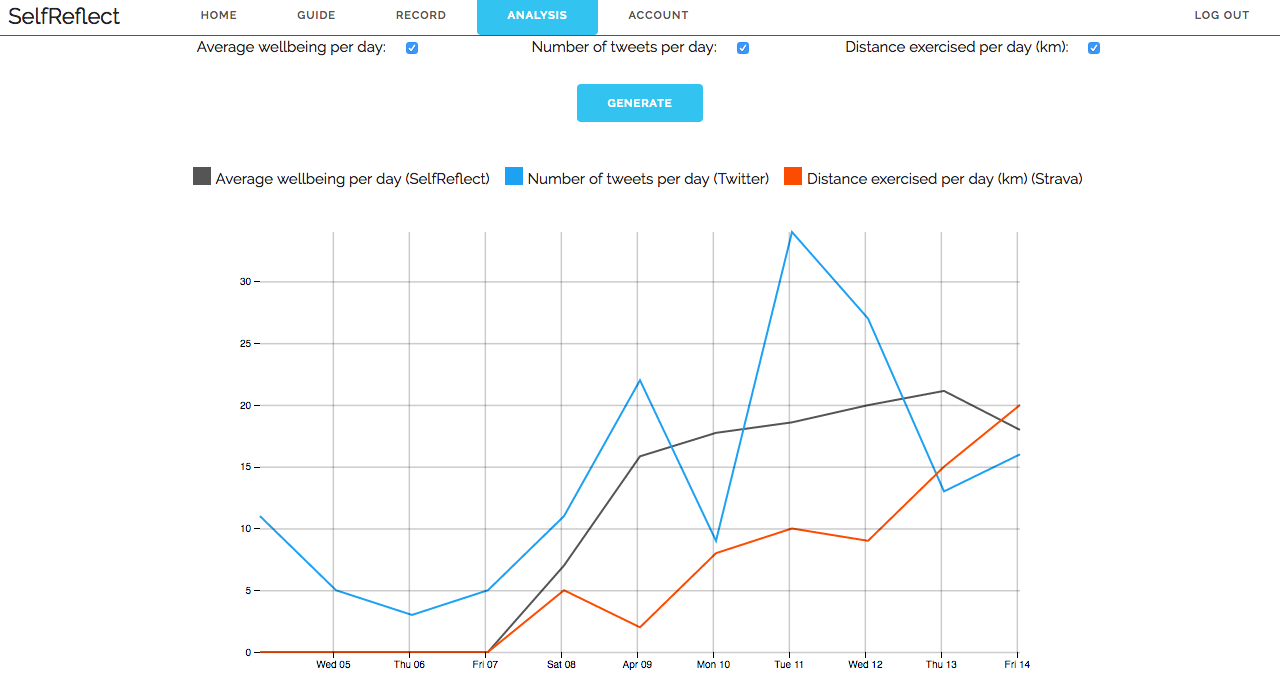
\includegraphics[width=\textwidth]{i/webanalysisgraph.png}
\label{fig:webanalysisgraph}
\end{figure}

\newpage
\subsection{Responsiveness}
Throughout development regular checks were made to ensure the web app was responsive and functional on various screen sizes. This required some basic CSS code and more importantly correct usage of the Skeleton CSS grid system. However, this code is not particularly complex or interesting, so some images proving this responsiveness have simply been included in appendix \ref{app:webresponsiveness}. The only element that doesn't resize for a small screen is the graph, for fairly obvious reasons.

\subsection{Documentation}
Like the mobile app, documentation includes a short description of SelfReflect and the SelfReflect web app, as well as instructions on how to install, set up and run the web app for local development and testing. This documentation can be seen in appendix \ref{app:webdocs}.

\section{API} \label{sec:apiimpl}
\subsection{Versioning}
Early in the implementation process of the API, versioning was added. This is the reason all endpoints start with \emph{/v1/}. The fact that this was not included in the original design was an oversight, as this is a common, best practise feature to add to modern APIs. It means that applications can be developed to work with the API without fear of continued development or breaking changes. If some change is made to improve the API that breaks backwards-compatibility, this can be created as a \emph{/v2/} endpoint. Existing applications that use the API can then choose to continue to use the old endpoint, or upgrade to the new endpoint with minimal downtime.

\subsection{Technologies and Basic Implementation}
The API was developed using the technologies discussed in section \ref{sec:apidesign}: Node.js, Express and MySQL. Express is used to generate a base app. Callback functions can then be attached to this base app to define the endpoints of the API. These define what to do when each endpoint is hit. The app is then set to listen on a specific port. An example of this (which is a subset of the SelfReflect API code) can be seen below. This example includes adding the \emph{POST /v1/tokens} endpoint to the express app.
\begin{lstlisting}
let app = express()

...

app.post('/v1/tokens', (req, res) => {
  createToken(req.body, res)
})

...

/* Start server */
const server = app.listen(3000)

console.log('Express server started on port %s', server.address().port)

export default server
\end{lstlisting}

\subsection{Tokens Endpoints and Authenticating Requests}
\subsubsection{Generating and Refreshing Tokens}
The tokens endpoints handle the validation of credentials, and generation of tokens. The most significant endpoint is \emph{POST /v1/tokens}. This receives email and password, then checks the email exists and the password is correct. If either of these fail, it responds with a \emph{403 (Forbidden)} error. If both succeed, it uses an open source library called \enquote{node-jsonwebtoken} \parencite{nodejwt} to sign and generate a JSON Web Token. The following code generates the token, and sets it in the response:
\begin{lstlisting}
const generateToken = (id, expiry, res) => {
  jwt.sign({ id: id, exp: expiry }, secret, {}, (err, token) => {
    ...

    res.status(200).json({ id, token, exp: expiry })
  })
}
\end{lstlisting}

This generates the token using a secret, which is stored on the server and is kept private. This is just a string used to generate and verify tokens. This function also takes an expiry parameter, which is set to the current time plus one day (in seconds). The object that is encrypted in the token contains the expiry and the user id of the user with the given email and password.

In the case of a PUT \emph{/v1/tokens} request, email and password are not required. If a valid token is set in the request header, this is enough to authenticate the request, so a fresh token can be sent in the response, with the same user id as the provided token.

\subsubsection{Authenticating Requests and Accessing Restricted Endpoints}
As discussed in the design section of the api (section \ref{sec:apisecurity}), many endpoints require authentication as they access or modify user's data. The token, obtained from valid requests to the \emph{/v1/tokens} endpoints, must be sent in the \emph{Authorization} header of all requests to restricted endpoints. All \emph{/v1/users/:id} endpoints are restricted. The only users endpoint that is not restricted is \emph{/v1/users} (for account creation), as the user cannot authenticate if they do not have an account.

In order to add this check to all of the required endpoints, \enquote{middleware} was used. This middleware sits between the received request and the callback functions for each endpoint. Another piece of open source software called \enquote{express-jwt} \parencite{expressjwt} was used to achieve this. The usage of this can be seen in the following code:
\begin{lstlisting}
// Decode Authorization header token
const jwtMiddleware = jwt({
  secret: secret,
  requestProperty: 'token'
})

// Apply to all paths except "/users" and "POST /tokens"
app.use(jwtMiddleware.unless({
  path: [
    '/v1/users',
    { url: '/v1/tokens', methods: ['POST'] }
  ]
}))

// Error handling
app.use((err, req, res, next) => {
  if (err.name === 'UnauthorizedError') {
    return res.status(401).json({ error: 'Unauthorized' })
  }
})
\end{lstlisting}
This intercepts all endpoints other than \emph{/v1/users} (for user creation), and \emph{POST /v1/tokens}, as this does not require a token to be provided. The middleware will then throw an \enquote{UnauthorizedError} unless both of the following conditions are met:
\begin{itemize}
\item A token is provided.
\item The token is valid, i.e. can be decoded using the server secret.
\end{itemize}

The decoded token is then passed to the callback function, as part of the request. This can then be used to perform extra checks. In the case of the SelfReflect API, this is used to check that the user id in the token is the same as the user id of the requested resource. An example of this can be seen below:
\begin{lstlisting}
app.get('/v1/users/:id', (req, res) => {
  const id = parseInt(req.params.id, 10)

  if (!isValidId(id)) {
    return res.status(404).json({ error: 'Invalid user id' })
  }

  if (req.token.id !== id) {
    return res.status(403).json({ error: 'Forbidden' })
  }

  getUser(id, res)
})
\end{lstlisting}

This checks the user id is valid, then checks the user id matches that of the requested resource. Combining this token generation and authentication middleware provides all authentication required for restricted endpoints in the SelfReflect API.

\subsection{Secure Password Storage}
In order to implement secure password storage and hashing, as described in section \ref{subsec:secpass}, an open source library called \enquote{node.bcrypt.js} was used, which simply implements \emph{bcrypt} hashing and is compatible with Node.js \parencite{nodebcrypt}. This is implemented using the following code:
\begin{lstlisting}
const saltRounds = 10
...
bcrypt.hash(password, saltRounds, (err, hash) => {
  ...
  connection.query(
    'INSERT INTO user (email, password, twitter_username) VALUES (?, ?, ?)',
    [email, hash, twitter],
    (err, result) => {
      ...
    }
  )
})
\end{lstlisting}
This is the code used to create a user in the database. This hashes the password, then inserts the resultant hash in the database in the password field for the user. Note that this library automatically generates and uses a salt. Salt rounds can be increased or decreased; more salt rounds provides added security at the cost of processing speed. Ten salt rounds is the default that is recommended by the author of the open source library, so this was used for the SelfReflect API.

\subsection{Users Endpoints} \label{sec:apiimplusers}
The endpoints implemented are almost identical to those described in section \ref{sec:apiendpoints}. They will not all be described in detail here as are very simple and intuitive, and hence the code is not particularly interesting. Creation of users for example consists of a simple function that extracts email and password from the request, performs some validation (checks fields exist, checks email not already in use), then performs a simple MySQL insert to insert an entry into the database. Full descriptions of all of these endpoints have been detailed in the documentation, as discussed in section \ref{sec:apidocs}. The only endpoints that will be discussed in detail here are those that relate to external APIs (Twitter and Strava).

\subsection{Twitter} \label{sec:apiconnecttwitter}
\subsubsection{Connect Twitter}
As discussed in the web app implementation section (section \ref{subsec:webconnectapis}), Twitter provides application only authentication. For this reason only a user's Twitter username was required, and so this simply became part of the users endpoint. Rather than user specific access tokens being required, an application level access token is used. This is obtained on Twitter's developer website, by creating an account and an application. Twitter then provide a key and secret, which can be exchanged for an application level access token.

\subsubsection{Fetch Tweets}
Once the application level access token is obtained, and a user's Twitter username is provided, the user's timeline can be fetched. This is done using the following code:
\begin{lstlisting}
import { twitterAPI, token } from '../../config/twitter'

...

export const getTwitterData = (id, res) => {
  getUserById(id, (err, user) => {

  ...

  const query = '?count=200&trim_user=true&exclude_replies=true&screen_name='

  fetch(twitterAPI + query + twitterUsername, {
    method: 'GET',
    headers: {
      'Content-Type': 'application/json',
      'Authorization': 'Bearer ' + token
    }
  })
    .then(response => {
      ...
    })
})
\end{lstlisting}
This code fetches the user's timeline using the Twitter API. The token variable in this case contains the application level access token. For maximum extensibility, the Twitter timeline data is returned \enquote{raw}. That is, unmodified from the format provided by Twitter.

\subsection{Strava} \label{sec:apiconnectstrava}
\subsubsection{Connect Strava}
The SelfReflect API must handle exchanging the code given from the Strava user authorisation page for an access token for that user. To do this, it must post this code to a specific Strava API endpoint. This is done by the following code:
\begin{lstlisting}
import { stravaTokenAPI, clientId, clientSecret } from '../../config/strava'
...
export const updateStravaToken = (id, code, res) => {
  if (!code) {
    return res.status(400).json({ error: 'No Strava code provided' })
  }

  getUserById(id, (err, user) => {
    ...
    fetch(stravaTokenAPI, {
      method: 'POST',
      headers: {
        'Content-Type': 'application/json'
      },
      body: JSON.stringify({
        'client_id': clientId,
        'client_secret': clientSecret,
        code
      })
    })
      .then(response => {
        ...
      })
  })
})
\end{lstlisting}
The client id and client secret are obtained, like Twitter, by signing up to Strava's developer site and registering an application. The code above can then obtains an access token for this user in exchange for the code, and store this access token in the SelfReflect database against that user.

\subsubsection{Fetch Strava Data}
Once an access token is obtained and stored, it can be used in subsequent requests to fetch the users data. In the case of SelfReflect, this fetches the user's \enquote{activities}. The code to do this is shown below:
\begin{lstlisting}
import { stravaDataAPI, clientId, clientSecret } from '../../config/strava'

export const getStravaData = (id, res) => {
  getUserById(id, (err, user) => {
    ...
    const stravaToken = user.strava_token

    if (!stravaToken) {
      return res.status(400).json({
        error: 'Strava not connected for this user'
      })
    }

    fetch(stravaDataAPI, {
      method: 'GET',
      headers: {
        'Content-Type': 'application/json',
        'Authorization': 'Bearer ' + stravaToken
      },
      body: JSON.stringify({
        'per_page': 200
      })
    })
      .then(response => {
        ...
      })
  })
})
\end{lstlisting}

This is very similar to the code to fetch a user's Twitter timeline, with a few changes. The API is different of course, and the token in the \enquote{Authorization} header is different. This is loaded from the database, and is user specific rather than application-level. As with Twitter data, the Strava data is returned \enquote{raw} i.e. unmodified from the format provided by Strava.

\subsection{Documentation} \label{sec:apidocs}
A huge amount of documentation was written for the SelfReflect API. This documentation includes:
\begin{itemize}
\item A short description of SelfReflect and the SelfReflect API.
\item Instructions on how to install, set up and run the API for local development and testing.
\item Instructions on how to run the automated tests.
\item Specific details and instructions on how API authentication works.
\item Documentation for every endpoint, including:
  \begin{itemize}
  \item The name, method (GET, POST etc.), and URI of the endpoint.
  \item Whether or not this endpoint requires an authentication token (is restricted).
  \item A description of what this endpoint is used for.
  \item The body field(s) required in the body of a request to this endpoint, if any.
  \item All possible error responses, including status codes, messages and the reason for these errors.
  \item Information about the success response, including status code and an example success response body.
  \end{itemize}
\end{itemize}

This full documentation is very large, and can be seen in appendix \ref{app:apidocs}.

\section{Database}
The database was implemented almost exactly as discussed in the database design section (section \ref{sec:databasedesign}), using MySQL. The only change relates to the change in how Twitter was connected for a user. The Twitter token column in the users table was simply renamed to \emph{twitter\textunderscore username}. The final entity-relationship diagram for the implemented database can be seen in Figure \ref{fig:dberdimpl}.

\begin{figure}[ht]
\centering
\caption{Implemented Database Entity-Relationship Diagram}
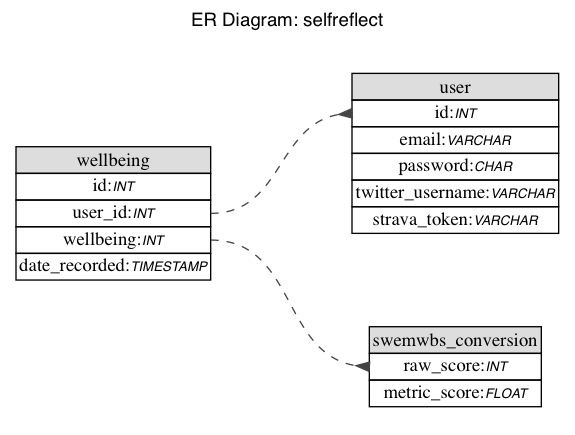
\includegraphics[width=0.8\textwidth]{i/dberdimpl.png}
\label{fig:dberdimpl}
\end{figure}

\chapter{Testing}
\section{Introduction}
Throughout the entire implementation of the project, manual testing was carried out to check all functionality was working and was implemented correctly. However, this is not sufficient to fully test the system. In order to do this, two further types of testing were carried out: automated testing for the API, and user testing for the entire system. The API is tested indirectly by user testing, but cannot be tested directly by users, so automated testing was implemented. This was essential as the API deals with user data, security and authentication. These are very important features and so it was essential to test these, and ensure the implemented code works correctly and reliably.

\section{Automated Testing}
\subsection{Technologies}
To implement tests for the API, various open source libraries were used:
\begin{enumerate}
\item \emph{Mocha}: A \enquote{feature-rich JavaScript test framework running on Node.js and in the browser, making asynchronous testing simple and fun} \parencite{mocha}. This is the basic framework used for writing the tests.
\item \emph{Chai}: An \enquote{assertion library for node} \parencite{chai}. This makes some assertions more readable and easier to understand.
\item \emph{Istanbul}: Used for code coverage calculation and reports. \enquote{Istanbul instruments your ES5 and ES2015+ JavaScript code with line counters, so that you can track how well your unit-tests exercise your codebase} \parencite{instanbul}.
\item \emph{Supertest}: A \enquote{high-level abstraction for testing HTTP} \parencite{supertest}. Used for writing \enquote{API tests} which send HTTP requests to the SelfReflect API.
\end{enumerate}

\subsection{Method}
The details of all the tests and their specific implementation will not be discussed here. A set of tests were written for each endpoint, so that for every endpoint:
\begin{itemize}
\item The expected success response was tested.
\item Every error response to a valid request was tested, such as duplicate emails (providing a duplicate email is a valid request that returns an error response).
\item Every error response to invalid request was tested, such as requesting information for a user id that is not authenticated, or providing no authentication token.
\end{itemize}

In order to test some more complicated endpoints, such as Twitter and Strava, test accounts had to be created for each of these applications. The tests could then use these accounts, and as these accounts are controlled, assertions could be made on the expected response from Twitter and Strava.

\subsection{Code Coverage}
In the requirements section for the API (section \ref{subsec:apireqs}), non-functional requirements 6.1 and 6.2 relate to covering at least 70\% and 95\% of lines of testable code respectively. The reason the word testable was included here is because some lines are near impossible to \emph{meaningfully} test. An example of this is an error thrown by the operating system. Another might be errors thrown by MySQL itself, if the database becomes inaccessible for whatever reason. This is almost impossible to recreate in a test case without making the test arbitrary and meaningless. In order to remove these lines from the code coverage calculation, Istanbul can be told to ignore specific lines using specific code comments.

Once these very limited scenarios were ignored from the code coverage calculation, only testable lines of code remained. The automated tests managed to cover all of these testable lines, achieving 100\% test coverage and satisfying both non-functional requirements 6.1 and 6.2. The code coverage report proving this test coverage is shown in Figure \ref{fig:codecoverage}.

\begin{figure}[ht]
\centering
\caption{API 100\% Lines Code Coverage Report}
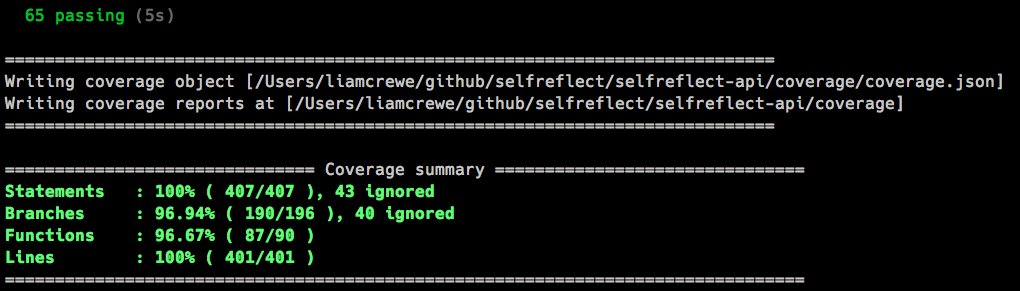
\includegraphics[width=\textwidth]{i/codecoverage.png}
\label{fig:codecoverage}
\end{figure}

\newpage
\section{User Testing} \label{sec:usertesting}
The user testing of the system was designed with three key goals in mind:
\begin{enumerate}
\item Test the \emph{functionality} of the system. That is, check that users can successfully use all the implemented features of the system.
\item Test the \emph{usability} of the system. That is, check how easy it is for users to use the various features of the system, and get feedback on how this could be improved.
\item Get suggestions for improvements and additional features from users who have tested the system.
\end{enumerate}

In order to test these, volunteer users were asked to carry out a series of tasks for the mobile app, then a series of tasks for the web app. These tasks can be seen in appendix \ref{app:testing:tasks}. In order to test the visualisations properly, an account with data already on it was required. For this reason, a test account was created, with some wellbeing data already created in the SelfReflect database, and with existing Twitter and Strava accounts already connected. Any failures or errors that occurred in simply carrying out these tasks were recorded, covering goal 1. Users were then asked to answer a questionnaire, with a set of questions for each of the mobile and web app. These questions were designed to cover goals 2 and 3. Some questions asked the user how easy it was to carry out the separate tasks, on a simple one to five scale (goal 2), while others asked the user to report any issues they found and for suggestions for improvements and additional features (goal 3). This questionnaire can be seen in appendix \ref{app:testing:questionnaire}.

This testing was carried out by a number of volunteers. Research carried out by \citeauthor{nielsenfiveusers} (\citeyear{nielsenfiveusers}) recommended using five users. This article stated that testing with five users \enquote{lets you find almost as many usability problems as you'd find using many more test participants}. However, the testing carried out in this project was not just usability testing; it also tested functionality and aimed to get suggestions from users, as discussed above. For this reason, ten users were selected to carry out the user testing and answer the questionnaire. These users were of a variety of ages, and had a variety of technical proficiency levels.

\chapter{Results and Discussion} \label{chap:results}
The complete results of the testing can be seen in appendix \ref{app:testing:results}. These results will be discussed for each of the mobile app and web app, with reference to the goals of the user testing as detailed in section \ref{sec:usertesting}. These are, in short: functionality, usability, and improvements and/or additional features.

\section{Functionality Testing}
The initial plan was to record any failures or errors that occurred while users were carrying out the set of testing tasks. However, none of these failures or errors occurred; all ten volunteer test users managed to complete the entire set of tasks successfully, for both the mobile app and the web app, albeit some users slower than others.

\section{Mobile App}
The first three mobile app questions used a scale of one to five, where one is \enquote{very easy} and five is \enquote{very difficult}. Of these questions, the vast majority of answers were rated one or two. Also, for the fourth question, all users responded stating the table was either \enquote{very clear} or \enquote{clear}. These results suggest that the overall usability of the system was very good. However, some answers did highlight usability issues and areas for improvement. The answers for the first three questions that were greater than two will be discussed in the following section, as well as other usability issues identified, including why the user found this an issue, and what could be done to improve usability. These future usability changes will then be summarised in section \ref{subsec:mobusabilityimp}.

\subsection{Usability Testing Issues}
\subsubsection{Account Creation}
One user answered four for the \enquote{create an account} task. This same user answered the question regarding issues with the mobile app with the statement \enquote{confused by being on log in screen when asked to create an account}. This related more to the testing process than the app itself. As the user had the task of creating an account in mind, they expected the account creation screen to be the first screen they saw, rather than having to find it. This could be resolved by simply having a more clear testing process, by explaining the process more thoroughly to the user, having clearer instructions, or setting the first screen the user sees as the registration screen.

\subsubsection{Recording Wellbeing}
Two users answered three for the \enquote{record your wellbeing} task. These users explained this (in the question about issues with the mobile app) by saying they were a little confused how to record wellbeing from the home screen, and by stating that their initial instinct was to try to fill out the \enquote{last 5 recordings} table rather than press the record button. These users suggested that the record button could be made more obvious, by making it bigger, brighter or highlighting it somehow.

\subsubsection{Log Out}
Another usability issue identified by testers related to logging out of the application. Users tended to notice the log out \enquote{symbol}, but thought it was a power symbol for the device, not a log out button. They therefore spent a long time deliberating before trying the log out button to see if that was the correct way to log out. Although users managed this eventually without help, many suggested that this could be clearer. The overwhelming majority of the user that suggested this stated that including the words \enquote{log out}, either next to or instead of the symbol, would improve the usability of the system.

\subsection{Summary of Future Usability Improvements} \label{subsec:mobusabilityimp}
Given the feedback on the usability of the system, the following changes could be made in future iterations of the SelfReflect mobile app:
\begin{itemize}
\item Make buttons (particularly record button) bigger and more obvious.
\item Change log out button to have the words \enquote{log out} written next to it, or even replace the symbol completely with the words \enquote{log out}.
\end{itemize}

\subsection{Summary of Improvements and/or Additional Features}
The last two questions in the mobile app section asked for: suggestions for improvements that could be made to existing features, and suggestions for additional features the user would like added to the mobile app. A summary of the suggestions obtained from the responses to these questions can be seen below:
\begin{itemize}
\item Improvement: Add a link to the web app to the message that encourages users to visit the SelfReflect web app.
\item Additional feature: Account management. Two users suggested this, with one requesting the entire account tab from the web app be added, and the other simply requesting the ability to change email and password. Either way, account management could be a useful feature to be added in future iterations of the SelfReflect mobile app.
\item Improvement: One user suggested the SelfReflect title could be a logo or could use a more interesting font. This is something that would very likely be improved in future development of the system, and the very simple logo was used as a \enquote{placeholder} as this system was developed as a proof of concept.
\end{itemize}

\section{Web App}
The first seven mobile app questions used the scale of one to five. Again the vast majority of answers were one or two. In fact, the web app responses were even more positive than that of the mobile app. Only one user answered three or above for only one of the questions, as will be discussed in the following section, along with other usability issues identified, and the changes that could be made to improve usability. As with the mobile app, these future usability changes will be summarised in section \ref{subsec:webusabilityimp}.

\subsection{Usability Testing Issues}
\subsubsection{Edit Email and/or Password}
One user answered three for the \enquote{change email or password} question. This user answered the question regarding issues with the web app by stating the edit email/password buttons were a little hard to find. This could be an outlier, as nine out of ten users responded with two or below. Also, this user responded with three, so this is still a relatively good score. However, this result cannot be ignored and so the edit buttons could potentially be improved by making them bigger or more obvious in some way.

\subsubsection{Form Submission Success Messages}
Some responses to the questionnaire noted that the \enquote{success} messages for form submissions (i.e. register, edit email, edit password) were quite small and not too clear. This could therefore be improved by making the success message larger and bolder (increasing the font weight).

\subsection{Summary of Future Usability Improvements} \label{subsec:webusabilityimp}
Given the feedback on the usability of the system, the following changes could be made in future iterations of the SelfReflect web app:
\begin{itemize}
\item Make edit email and password buttons bigger and more obvious.
\item Make success form submission messages more noticeable, by making them larger and by increasing the font weight to make them bolder.
\end{itemize}

\subsection{Summary of Improvements and/or Additional Features} \label{subsec:addsources}
\subsubsection{General Web App}
The two questions for the mobile app that asked suggestions for improvements and/or additional features were also asked for the web app. A summary of the suggestions obtained from the responses to these questions can be seen below:
\begin{itemize}
\item Improvement: Make the guide page more interesting. This could be done by adding images, colour or simply structuring the page slightly differently.
\item Improvement: More interesting SelfReflect logo or font. As with the mobile app, this is something that would very likely be improved in future development of the system.
\item Additional feature: Different graphs types, formats and display options, such as pie charts and bar charts. Several users suggested this, and it would definitely be an area for development in future iterations of the SelfReflect web app.
\item Additional feature: Export facility for generated visualisations. The user could download an image of the generated graph to show to a professional to analyse. Another option for this is the ability to download the graph data as a csv file (comma separated values file), which could be imported into other systems.
\end{itemize}

\newpage
\subsubsection{Additional Sources}
The second last question of the questionnaire asked users for suggestions for additional sources. These suggestions are summarised below:
\begin{itemize}
\item Music based apps: Spotify, Apple music.
\item Extra social media apps: Facebook, Instagram.
\item Extra fitness apps: Fitbit, Garmin fitness, smart watches.
\item Diet and food tracking apps.
\item Sleep and sleeping pattern tracking apps.
\item Entertainment apps: Netflix or game usage.
\end{itemize}

\subsubsection{Additional Options Within Existing Sources}
The last question of the questionnaire asked users for suggestions for additional options \emph{within} existing sources. These suggestions are summarised below. It is possible that not all of these options are provided by Twitter/Strava, but these were suggested from users as areas to investigate as possible future additions.
\begin{itemize}
\item Twitter: Number of likes, retweets, replies, individual tweets or times refreshed, time spent on app without posting.
\item Strava: Pace analysis, time exercised per day, distance ran/cycled/swam per day, number of steps, time at rest, calories burned per day.
\end{itemize}

\section{Contributions to Research} \label{sec:contr}
Another important aspect to discuss with regard to these results is where, how and to what extent this project has contributed to the research discussed in the literature survey (chapter \ref{litsurvey}). Some parts of the survey helped with design aspects of the system and so are not relevant here, such as how to record wellbeing and the use of the SWEMWBS questionnaire. Others however identified and discussed the fields of research in which this project hoped to contribute. The key examples of these are:
\begin{itemize}
\item Mental health and self management.
\item Personal informatics in the context of mental health and wellbeing.
\item Visualisations.
\item Existing systems.
\end{itemize}

\subsection{Mental Health and Self Management}
Research showed that self management is \enquote{increasingly popular} \parencite{selfhelpanxiety} and has been shown to be effective in both treatment \parencite{wrapstudy} and \parencite{selfmanagementrelapse}. It investigated various techniques and found that all self management schemes had several features in common. They all required identification of events that can cause negative consequences, recognition of when these events occur and what effect they have, and planned actions to minimise the negative consequences of these events. This project planned to develop a system to aid with the first two of these. Users would be able to build graphs to identify events, identify when they occur and see visual proof of the effect this event had.

On one hand this can be considered a successful contribution for this project; a tool was successfully built to allow users to generate these graphs, allowing the possibility to identify the factors discussed. However, whether SelfReflect (in its current state) produces visualisations that are clear enough for the average user to identify these factors is, as of yet, untested. Future work should be carried out to discover if the average user can draw valid and useful conclusions, and ways in which the system can be improved to aid users in achieving this goal.

\subsection{Personal Informatics in the Context of Mental Health}
The literature survey discussed the five stage model of personal informatics systems by \citeauthor{li2010stage} (\citeyear{li2010stage}). It also stated which of these stages were primary focuses of this project: collection, integration and reflection. It then continued to discuss the impact of both social media activity and exercise on mental health and wellbeing, with the plan to develop a system to identify the exact nature of these relationships.

SelfReflect's implemented features cover all of these areas. The combination of the mental health SWEMWBS questionnaire, connecting of Twitter and Strava, the API and the visualisations cover all three of the stated stages of the five stage model. The visualisations allow graphs to be produced to potentially identify relationships between social media activity, exercise activity and mental health and wellbeing. However, much like the field of self management, future work should investigate how effective the system is in allowing users to identify these relationships, and how it could further help users to do so.

\subsection{Visualisations}
Another identified area in which this project hoped to contribute was by trialling a new method of presenting visualisations to the user. Rather than trying to guess which visualisations the user wanted, or identifying correlations automatically, this project planned to implement a tool to allow the user to generate visualisations themselves.

This was overall very successful; all users managed to generate visualisations across both two and three sources. Questionnaire responses showed that seven out of ten users rated this \enquote{very easy} to use, and the other three rated it \enquote{easy}. This means that overall, users found it simple and easy to generate visualisations across multiple sources. However, again further work should be carried out to investigate if users can identify correlations in data themselves, without the need for automatic identification.

\subsection{Existing Systems}
Finally, the literature survey reviewed existing systems and defined how SelfReflect would differentiate itself from these systems. It planned to do this by combining user submitted mental health and wellbeing data with API data, and by implementing a simple visualisation building tool.

Both of these goals have already been discussed above, and it is clear that this system managed to achieve both of these with the features implemented. Providing no substantial systems were missed during research, SelfReflect can be said to be a unique system that contributes to the fields discussed, in a way that these existing systems do not.

\chapter{Conclusion and Future Work} \label{chap:conc}
\subsection{Conclusion}
This project investigated the huge scale of the problem of mental health conditions in the UK, and the lack of funding faced by mental health services. It identified self management as a way to reduce the demand for mental health services, in people that are in of treatment, out of treatment and are post treatment. It also discussed personal informatics and its relation to mental health, as well as the modern state of user data, including the many apps that both record data about users, and make this data accessible via open APIs.

This project aimed to take advantage of this data by building a software system to aid in the self management of mental health, called SelfReflect. SelfReflect allows users to record their mental wellbeing and, via the use of personal informatics and ecological momentary assessment, produce visualisations to identify relationships between their mental wellbeing and data fetched from existing external apps.

The literature survey found that helping a user to understand their mental health, and involving them in treatment, can be hugely beneficial to their recovery. It identified the government developed and tested SWEMWBS questionnaire as the best method for recording wellbeing. It also provided further insight into the field of personal informatics, both in general and in the context of mental wellbeing. Physical exercise and social media were identified as two example types of data that research suggests have some significant effect on mental wellbeing. It then identified four similar systems in the field, analysed these, and identified where SelfReflect could differentiate itself and contribute to the fields of mental health self management and personal informatics.

SelfReflect was then designed and implemented, which included three separate pieces of software. This consisted of an API and two client applications that communicate with the API: a mobile app and a web app.

The API handled authentication and data storage/retrieval, including storing credentials and fetching data from external APIs. The mobile app was  designed to be very simple, to allow account creation, log in and recording of wellbeing, with the goal of encouraging ecological momentary assessment. The web app was more complex, encompassing all features of the mobile app, as well as allowing account management (including connecting external APIs), and data analysis via a visualisation building tool.

The two sources implemented in this project were Twitter and Strava. One visualisation was included for each of these, and for SelfReflect itself: average wellbeing per day for SelfReflect, number of tweets per day for Twitter, and distance exercised per day (in km) for Strava. The scope of the system was defined very early in the project to only include these two sources and three visualisations. These two sources were implemented as proofs of concept, to investigate the possibility of building these visualisations, and to develop the base system. The entire software system was developed to be extensible; to be built on in future projects. For this reason suggestions for future work are important and key conclusions for this project.

The API was tested using automated tests, with the justification that it both deals with data storage/retrieval and cannot be tested directly manually. Ten volunteer users then carried user testing. This consisted of a set of tasks for each of the mobile and web app, and the answering of a questionnaire. This testing aimed to test the functionality and usability of the system, gather user's suggestions for improvements and/or additional features to the software, and gather user's suggestions for additional sources and/or additional visualisations for existing sources. These responses were then collated, discussed, summarised and identified as areas of future work that could improve or expand the system.

SelfReflect provides a hugely extensible framework for future development, including testing and extensive documentation. Two sources have been connected already, and a visualisation building tool has been implemented, that could allow users to identify activities that positively or negatively affect their mental wellbeing. This provides a base system for future work, that could expand SelfReflect into an \emph{extensive} personal informatics system to aid in the self management of mental health and wellbeing.

\subsection{Future Work}
There are three key areas for future work: system improvements and additional features, system source expansion and system feasibility research.

\subsubsection{System Improvements and Additional Features}
These were detailed and summarised in the results and discussion chapter of this project (chapter \ref{chap:results}). This consists of further development to improve the usability of the system, as well as additional features such as account management for the mobile app, and export functionality for visualisations.

\subsubsection{System Source Expansion}
This is, and was always going to be, a key area for future work for this project. Twitter and Strava were included as proofs of concept, with one visualisations built for each. The system has been designed to be extensible to add lots more of these, in order to provide an extensive personal informatics system to aid in the self management of mental health and wellbeing. Users provided a large number of suggestions for these, both in terms of additional sources and/or visualisations within existing sources, as seen in section \ref{subsec:addsources}.

\subsubsection{System Feasibility Research}
Either using the current system, or after further projects to improve and expand the software system, the feasibility of the software as a tool to aid in the self management of mental health and wellbeing needs to be investigated. This would need to be an organised, controlled study to measure the effectiveness of the system. This is somewhat similar to the suggestions made in section \ref{sec:contr}, regarding the contributions of this project to existing research, and how it could contribute further in future work. Possible aims of this research could be: to investigate how effective the system can be as a tool for those who are suffering from mental health conditions or poor mental wellbeing, to investigate which users it would be most useful for, to gather the opinion of mental health specialists on the feasibility of the system, and many others. Most importantly however, future research should establish whether SelfReflect, or an expanded version of it, could truly help to tackle the huge problem of poor mental health and wellbeing in the UK, and whether this could reduce the demand for treatment from the underfunded and oversubscribed NHS mental health services.

\printbibliography

\begin{appendices}
\section{SWEMWBS conversion table} \label{SWEMWBS conversion table}
\begin{figure}[ht]
  \centering
  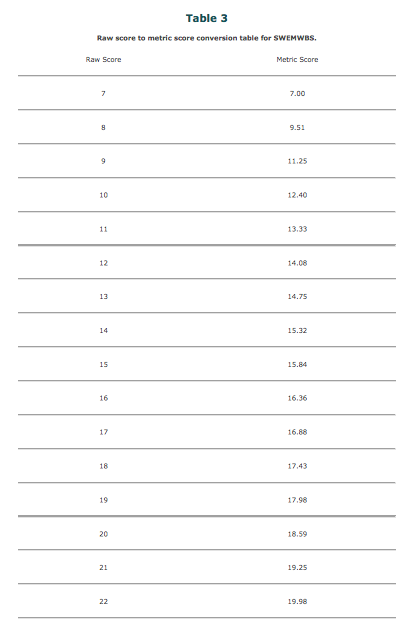
\includegraphics[width =.7\textwidth]{i/swemwbsconversiontable1.png}
  \label{swemwbsconversiontable}
\end{figure}

\newpage
\begin{figure}[ht]
  \centering
  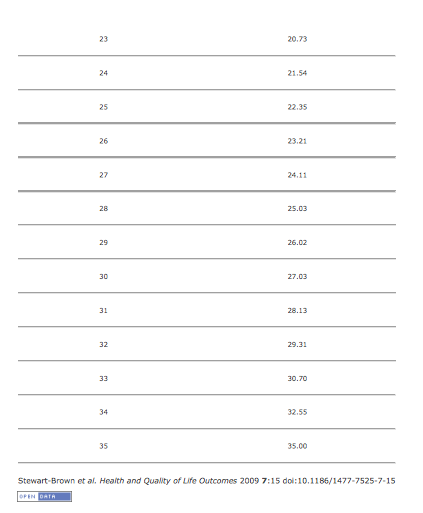
\includegraphics[width =.7\textwidth]{i/swemwbsconversiontable2.png}
\end{figure}

\newpage
\section{Mobile App Documentation} \label{app:mobiledocs}
\begin{figure}[ht]
  \centering
  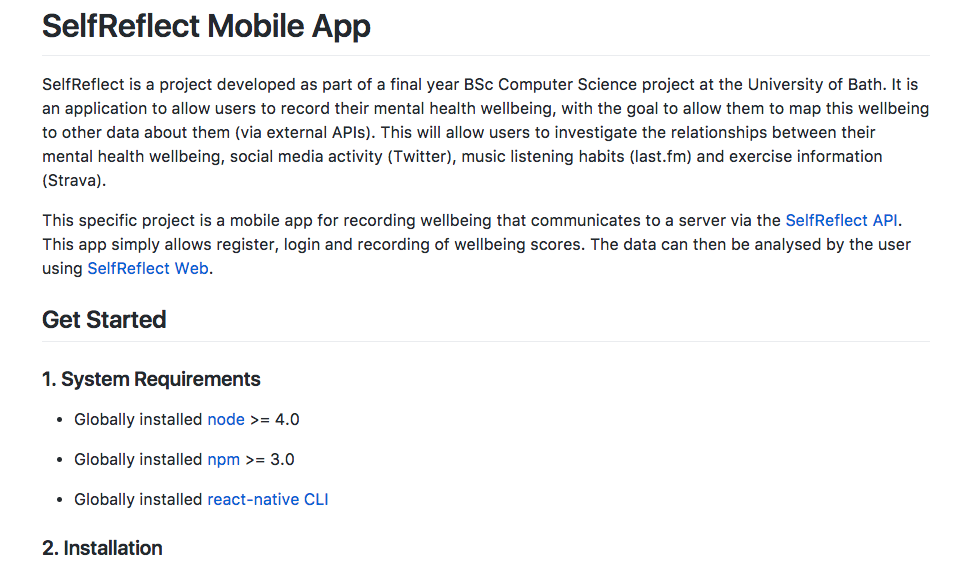
\includegraphics[width=.9\textwidth]{i/mobiledocs1.png}
\end{figure}

\begin{figure}[ht]
  \centering
  \includegraphics[width=.9\textwidth]{i/mobiledocs2.png}
\end{figure}

\newpage
\section{Web App Responsiveness} \label{app:webresponsiveness}
\begin{figure}[ht]
  \centering
  \includegraphics[width=.3\textwidth]{i/webresp1.png} \hfill
  \includegraphics[width=.3\textwidth]{i/webresp2.png} \hfill
  \includegraphics[width=.3\textwidth]{i/webresp3.png}
\end{figure}

\begin{figure}[ht]
  \centering
  \includegraphics[width=.3\textwidth]{i/webresp4.png} \hfill
  \includegraphics[width=.3\textwidth]{i/webresp5.png} \hfill
  \includegraphics[width=.3\textwidth]{i/webresp6.png}
\end{figure}

\newpage
\section{Web App Documentation} \label{app:webdocs}
\begin{figure}[ht]
  \centering
  \includegraphics[width=.9\textwidth]{i/webdocs1.png}
\end{figure}

\newpage
\begin{figure}[ht]
  \centering
  \includegraphics[width=.9\textwidth]{i/webdocs2.png}
\end{figure}

\section{API Documentation} \label{app:apidocs}
\begin{figure}[ht]
  \centering
  \includegraphics[width=.9\textwidth]{i/apidocs1.png}
  \includegraphics[width=.9\textwidth]{i/apidocs2.png}
\end{figure}

\begin{figure}[ht]
  \centering
  \includegraphics[width=.9\textwidth]{i/apidocs3.png}
  \includegraphics[width=.9\textwidth]{i/apidocs4.png}
\end{figure}

\begin{figure}[ht]
  \centering
  \includegraphics[width=.9\textwidth]{i/apidocs5.png}
  \includegraphics[width=.9\textwidth]{i/apidocs6.png}
\end{figure}

\begin{figure}[ht]
  \centering
  \includegraphics[width=.9\textwidth]{i/apidocs7.png}
  \includegraphics[width=.9\textwidth]{i/apidocs8.png}
\end{figure}

\begin{figure}[ht]
  \centering
  \includegraphics[width=.9\textwidth]{i/apidocs9.png}
  \includegraphics[width=.9\textwidth]{i/apidocs10.png}
\end{figure}

\begin{figure}[ht]
  \centering
  \includegraphics[width=.9\textwidth]{i/apidocs11.png}
  \includegraphics[width=.9\textwidth]{i/apidocs12.png}
\end{figure}

\begin{figure}[ht]
  \centering
  \includegraphics[width=.9\textwidth]{i/apidocs13.png}
  \includegraphics[width=.9\textwidth]{i/apidocs14.png}
\end{figure}

\begin{figure}[ht]
  \centering
  \includegraphics[width=.9\textwidth]{i/apidocs15.png}
  \includegraphics[width=.9\textwidth]{i/apidocs16.png}
\end{figure}

\clearpage
\section{User Testing Tasks} \label{app:testing:tasks}
\begin{figure}[ht]
  \centering
  \includegraphics[width=.8\textwidth]{i/testingtasks.png}
\end{figure}

\clearpage
\section{User Testing Questionnaire} \label{app:testing:questionnaire}
\begin{figure}[ht]
  \centering
  \includegraphics[width=\textwidth]{i/testingquestionnaire1.png}
\end{figure}

\begin{figure}[ht]
  \centering
  \includegraphics[width=\textwidth]{i/testingquestionnaire2.png}
  \includegraphics[width=\textwidth]{i/testingquestionnaire3.png}
\end{figure}

\begin{figure}[ht]
  \centering
  \includegraphics[width=\textwidth]{i/testingquestionnaire4.png}
  \includegraphics[width=\textwidth]{i/testingquestionnaire5.png}
\end{figure}

\clearpage
\section{User Testing Questionnaire Responses} \label{app:testing:results}
\begin{figure}[ht]
  \centering
  \includegraphics[width=.9\textwidth]{i/testingresponses1.png}
\end{figure}

\begin{figure}[ht]
  \centering
  \includegraphics[width=.9\textwidth]{i/testingresponses2.png}
  \includegraphics[width=.9\textwidth]{i/testingresponses3.png}
\end{figure}

\begin{figure}[ht]
  \centering
  \includegraphics[width=.9\textwidth]{i/testingresponses4.png}
  \includegraphics[width=.9\textwidth]{i/testingresponses5.png}
\end{figure}

\begin{figure}[ht]
  \centering
  \includegraphics[width=.9\textwidth]{i/testingresponses6.png}
  \includegraphics[width=.9\textwidth]{i/testingresponses7.png}
\end{figure}

\begin{figure}[ht]
  \centering
  \includegraphics[width=.9\textwidth]{i/testingresponses8.png}
  \includegraphics[width=.9\textwidth]{i/testingresponses9.png}
\end{figure}

\begin{figure}[ht]
  \centering
  \includegraphics[width=.9\textwidth]{i/testingresponses10.png}
  \includegraphics[width=.9\textwidth]{i/testingresponses11.png}
\end{figure}

\begin{figure}[ht]
  \centering
  \includegraphics[width=.9\textwidth]{i/testingresponses12.png}
  \includegraphics[width=.9\textwidth]{i/testingresponses13.png}
\end{figure}

\begin{figure}[ht]
  \centering
  \includegraphics[width=.9\textwidth]{i/testingresponses14.png}
  \includegraphics[width=.9\textwidth]{i/testingresponses15.png}
\end{figure}

\end{appendices}

\end{document}
